\documentclass[a4paper,12pt,oneside,times,numbered,print,index]{Classes/PhDThesisPSnPDF}

% ******************************************************************************
% ******************************* Class Options ********************************
% *********************** See README for more details **************************
% ******************************************************************************

% `a4paper'(The University of Cambridge PhD thesis guidelines recommends a page
% size a4 - default option) or `a5paper': A5 Paper size is also allowed as per
% the Cambridge University Engineering Deparment guidelines for PhD thesis
%
% `11pt' or `12pt'(default): Font Size 10pt is NOT recommended by the University
% guidelines
%
% `oneside' or `twoside'(default): Printing double side (twoside) or single
% side.
%
% `print': Use `print' for print version with appropriate margins and page
% layout. Leaving the options field blank will activate Online version.
%
% `index': For index at the end of the thesis
%
% `draftclassic': For draft mode without loading any images (same as draft in book)
%
% `draft': Special draft mode with line numbers, images, and water mark with
% timestamp and custom text. Position of the text can also be modified.
%
% `abstract': To generate only the title page and abstract page with
% dissertation title and name, to submit to the Student Registry
%
% `chapter`: This option enables only the specified chapter and it's references
%  Useful for review and corrections.
%
% ************************* Custom Page Margins ********************************
%
% `custommargin`: Use `custommargin' in options to activate custom page margins,
% which can be defined in the preamble.tex. Custom margin will override
% print/online margin setup.
%
% *********************** Choosing the Fonts in Class Options ******************
%
% `times' : Times font with math support. (The Cambridge University guidelines
% recommend using times)
%
% `fourier': Utopia Font with Fourier Math font (Font has to be installed)
%            It's a free font.
%
% `customfont': Use `customfont' option in the document class and load the
% package in the preamble.tex
%
% default or leave empty: `Latin Modern' font will be loaded.
%
% ********************** Choosing the Bibliography style ***********************
%
% `authoryear': For author-year citation eg., Krishna (2013)
%
% `numbered': (Default Option) For numbered and sorted citation e.g., [1,5,2]
%
% `custombib': Define your own bibliography style in the `preamble.tex' file.
%              `\RequirePackage[square, sort, numbers, authoryear]{natbib}'.
%              This can be also used to load biblatex instead of natbib
%              (See Preamble)
%
% **************************** Choosing the Page Style *************************
%
% `default (leave empty)': For Page Numbers in Header (Left Even, Right Odd) and
% Chapter Name in Header (Right Even) and Section Name (Left Odd). Blank Footer.
%
% `PageStyleI': Chapter Name next & Page Number on Even Side (Left Even).
% Section Name & Page Number in Header on Odd Side (Right Odd). Footer is empty.
%
% `PageStyleII': Chapter Name on Even Side (Left Even) in Header. Section Number
% and Section Name in Header on Odd Side (Right Odd). Page numbering in footer


% ********************************** Preamble **********************************
% Preamble: Contains packages and user-defined commands and settings
% ******************************************************************************
% ****************************** Custom Margin *********************************

% Add `custommargin' in the document class options to use this section
% Set {innerside margin / outerside margin / topmargin / bottom margin}  and
% other page dimensions
\ifsetCustomMargin
  \RequirePackage[left=37mm,right=30mm,top=35mm,bottom=30mm]{geometry}
  \setFancyHdr % To apply fancy header after geometry package is loaded
\fi

% Add spaces between paragraphs
%\setlength{\parskip}{0.5em}
% Ragged bottom avoids extra whitespaces between paragraphs
\raggedbottom
% To remove the excess top spacing for enumeration, list and description
%\usepackage{enumitem}
%\setlist[enumerate,itemize,description]{topsep=0em}

% *****************************************************************************
% ******************* Fonts (like different typewriter fonts etc.)*************

% Add `customfont' in the document class option to use this section

\ifsetCustomFont
  % Set your custom font here and use `customfont' in options. Leave empty to
  % load computer modern font (default LaTeX font).
  %\RequirePackage{helvet}

  % For use with XeLaTeX
  %  \setmainfont[
  %    Path              = ./libertine/opentype/,
  %    Extension         = .otf,
  %    UprightFont = LinLibertine_R,
  %    BoldFont = LinLibertine_RZ, % Linux Libertine O Regular Semibold
  %    ItalicFont = LinLibertine_RI,
  %    BoldItalicFont = LinLibertine_RZI, % Linux Libertine O Regular Semibold Italic
  %  ]
  %  {libertine}
  %  % load font from system font
  %  \newfontfamily\libertinesystemfont{Linux Libertine O}
\fi

% *****************************************************************************
% **************************** Custom Packages ********************************

\usepackage{etoolbox}
\usepackage{comment}
\usepackage{bm}

\makeatletter
\appto{\appendices}{\def\Hy@chapapp{Appendix}}
\makeatother

\renewcommand{\chaptername}{Capítulo}

% ************************* Algorithms and Pseudocode **************************

%\usepackage{algpseudocode}


% ********************Captions and Hyperreferencing / URL **********************

% Captions: This makes captions of figures use a boldfaced small font.
%\RequirePackage[small,bf]{caption}

\RequirePackage[labelsep=space,tableposition=top]{caption}
\renewcommand{\figurename}{Fig.} %to support older versions of captions.sty


% *************************** Graphics and figures *****************************

%\usepackage{rotating}
%\usepackage{wrapfig}

% Uncomment the following two lines to force Latex to place the figure.
% Use [H] when including graphics. Note 'H' instead of 'h'
\usepackage{float}
\restylefloat{figure}

% Subcaption package is also available in the sty folder you can use that by
% uncommenting the following line
% This is for people stuck with older versions of texlive
%\usepackage{sty/caption/subcaption}
\usepackage{subcaption}

% ********************************** Tables ************************************
\usepackage{booktabs} % For professional looking tables
\usepackage{multirow}

%\usepackage{multicol}
%\usepackage{longtable}
%\usepackage{tabularx}


% *********************************** SI Units *********************************
\usepackage{siunitx} % use this package module for SI units

\DeclareSIUnit{\belmilliwatt}{Bm}
\DeclareSIUnit{\belcarrier}{Bc}
\DeclareSIUnit{\dBm}{\deci\belmilliwatt}
\DeclareSIUnit{\dBc}{\deci\belcarrier}

% ******************************* Line Spacing *********************************

% Choose linespacing as appropriate. Default is one-half line spacing as per the
% University guidelines

% \doublespacing
% \onehalfspacing
% \singlespacing


% ************************ Formatting / Footnote *******************************

% Don't break enumeration (etc.) across pages in an ugly manner (default 10000)
%\clubpenalty=500
%\widowpenalty=500

%\usepackage[perpage]{footmisc} %Range of footnote options


% *****************************************************************************
% *************************** Bibliography  and References ********************

%\usepackage{cleveref} %Referencing without need to explicitly state fig /table

% Add `custombib' in the document class option to use this section
\ifuseCustomBib
   \RequirePackage[square, sort, numbers, authoryear]{natbib} % CustomBib

% If you would like to use biblatex for your reference management, as opposed to the default `natbibpackage` pass the option `custombib` in the document class. Comment out the previous line to make sure you don't load the natbib package. Uncomment the following lines and specify the location of references.bib file

%\RequirePackage[backend=biber, style=numeric-comp, citestyle=numeric, sorting=nty, natbib=true]{biblatex}
%\bibliography{References/references} %Location of references.bib only for biblatex

\fi

% changes the default name `Bibliography` -> `References'
\renewcommand{\bibname}{Bibliografía}


% ******************************************************************************
% ************************* User Defined Commands ******************************
% ******************************************************************************

\usepackage{booktabs}% http://ctan.org/pkg/booktabs
\newcommand{\tabitem}{~~\llap{\textbullet}~~}

% *********** To change the name of Table of Contents / LOF and LOT ************

\renewcommand{\contentsname}{Índice}
\renewcommand{\listfigurename}{Índice de Figuras}
\renewcommand{\listtablename}{Índice de Cuadros}


% ********************** TOC depth and numbering depth *************************

\setcounter{secnumdepth}{2}
\setcounter{tocdepth}{2}


% ******************************* Nomenclature *********************************

% To change the name of the Nomenclature section, uncomment the following line

%\renewcommand{\nomname}{Symbols}


% ********************************* Appendix ***********************************

% The default value of both \appendixtocname and \appendixpagename is `Appendices'. These names can all be changed via:

%\renewcommand{\appendixtocname}{Lista de apéndices}
\renewcommand{\appendixname}{Apéndice}

% *********************** Configure Draft Mode **********************************

% Uncomment to disable figures in `draft'
%\setkeys{Gin}{draft=true}  % set draft to false to enable figures in `draft'

% These options are active only during the draft mode
% Default text is "Draft"
%\SetDraftText{DRAFT}

% Default Watermark location is top. Location (top/bottom)
%\SetDraftWMPosition{bottom}

% Draft Version - default is v1.0
%\SetDraftVersion{v1.1}

% Draft Text grayscale value (should be between 0-black and 1-white)
% Default value is 0.75
%\SetDraftGrayScale{0.8}


% ******************************** Todo Notes **********************************
%% Uncomment the following lines to have todonotes.

\ifsetDraft
	\usepackage[colorinlistoftodos]{todonotes}
	\newcommand{\mynote}[1]{\todo[author=FS,size=\small,inline,color=green!40]{#1}}
\else
	\newcommand{\mynote}[1]{}
	\newcommand{\listoftodos}{}
\fi

% Example todo: \mynote{Hey! I have a note}


% ************************ Thesis Information & Meta-data **********************
% Thesis title and author information, refernce file for biblatex
% ************************ Thesis Information & Meta-data **********************
%% The title of the thesis
\title{Construcción de un modelo de ingeniería de un radar FMCW}
%\title{Writing your PhD thesis in \texorpdfstring{\\ \LaTeX2e}{LaTeX2e}}
%\texorpdfstring is used for PDF metadata. Usage:
%\texorpdfstring{LaTeX_Version}{PDF Version (non-latex)} eg.,
%\texorpdfstring{$sigma$}{sigma}

%% Subtitle (Optional)
%\subtitle{Using the CUED template}

%% The full name of the author
\author{José Francisco Soler}

%% Department (eg. Department of Engineering, Maths, Physics)
\dept{Departamento de Ingeniería en Electrónica}

%% University and Crest
\university{Universidad de Buenos Aires}
% Crest minimum should be 30mm.
\crest{
\includegraphics[width=0.2\textwidth]{Logo2}}
%% Use this crest, if you are using the college crest
%% Crest long miminum should be 65mm
%\crest{\includegraphics[width=0.45\textwidth]{University_Crest_Long}}

%% College shield [optional] 
% Crest minimum should be 30mm.
\collegeshield{
\includegraphics[width=0.2\textwidth]{Logo1}}


%% Supervisor (optional)
%% for multiple supervisors, append each supervisor with the \newline command
\supervisor{\textbf{Ing. Adrián Rosa}}
%Prof. C.D. Supervisor\newline
%Prof. E.F. Supervisor\newline
\advisor{\textbf{Ing. Pablo Marino Belcaguy}}

%% Supervisor Role (optional) - Supervisor (default) or advisor
\supervisorrole{Director: }
%% if no title is desired:
% \supervisorrole{}

%% Advisor (optional)
%% for multiple advisors, append each advisor with the \newline command
%\advisor{Advisor 1\newline
%Advisors 2\newline
%Advisor 3\newline
%Advisor 4}
     
%% Advisor Role (optional) - Advisor (default) or leave empty
\advisorrole{Co-Director: }
%% if no title is required
% \advisorrole{}


%% You can redefine the submission text:
% Default as per the University guidelines:
% ``This dissertation is submitted for the degree of''
\renewcommand{\submissiontext}{Tesis de grado de }

%% Full title of the Degree
\degreetitle{Ingeniería en Electrónica}

%% College affiliation (optional)
%\college{King's College}

%% Submission date
% Default is set as {\monthname[\the\month]\space\the\year}
\degreedate{Noviembre 2017} 

%% Meta information
\subject{LaTeX} \keywords{{LaTeX} {PhD Thesis} {Engineering} {Universidad de Buenos Aires}}


% ***************************** Abstract Separate ******************************
% To printout only the titlepage and the abstract with the PhD title and the
% author name for submission to the Student Registry, use the `abstract' option in
% the document class.

\ifdefineAbstract
 \pagestyle{empty}
 \includeonly{Declaration/declaration, Abstract/abstract}
\fi

% ***************************** Chapter Mode ***********************************
% The chapter mode allows user to only print particular chapters with references
% Title, Contents, Frontmatter are disabled by default
% Useful option to review a particular chapter or to send it to supervisior.
% To use choose `chapter' option in the document class

% \ifdefineChapter
%  \includeonly{Chapter3/chapter3}
% \fi

% ******************************** Front Matter ********************************
\begin{document}
\maketitle

\tableofcontents
	% \newpage
\mainmatter

%*******************************************************************************
%*********************************** First Chapter *****************************
%*******************************************************************************

\chapter{Introducción}  %Title of the First Chapter

\ifpdf
    \graphicspath{{Chapter1/Figs/Raster/}{Chapter1/Figs/PDF/}{Chapter1/Figs/}}
\else
    \graphicspath{{Chapter1/Figs/Vector/}{Chapter1/Figs/}}
\fi

En este capítulo se presenta una reseña general de este trabajo de tesis. El mismo se encuentra dividido en tres secciones. Primero, se discuten los objetivos y motivaciones que dieron lugar a este trabajo. A continuación se introduce la metodología aplicada. Finalmente, se presentan los temas tratados en los distintos capítulos del documento.

%********************************** %Second Section  *************************************
\section{Objetivo de la Tesis} \label{sc:objective}

El presente trabajo de tesis responde a la motivación de modelizar, construir, medir y validar un prototipo de ingeniería de un radar FMCW para medir la matriz de dispersión de cuerpos. 

Se desea realizar una prueba de concepto sobre un prototipo básico que permita dar un primer paso en el camino hacia el desarrollo de un prototipo más avanzado que se desea montar sobre un dron.


%El presente trabajo de tesis responde a la motivación de modelizar, construir, medir y validar un prototipo de ingeniería de un radar FMCW de modo tal que sirva como prueba de concepto para un desarrollo a futuro con mayor escalibilidad utilizando instrumental más preciso para la medición de la matriz de dispersión de los cuerpos iluminados. El principal objetivo de las mediciones realizadas con dicho radar es el de determinar cuáles son las fuentes principales de incertidumbre a la hora de caracterizar el objeto iluminado.

% El presente trabajo de tesis responde a la motivación de armar un prototipo de desarrollo para determinar la factibilidad de la determinación de la matriz de dispersión 
% \mynote{Armar un prototipo de desarrollo para mostrar factibilidad en su uso para una aplicación dada con una incertidumbre dada y entonces escalabilidad. }


%********************************** %Third Section  *************************************
\section{Metodología de la tesis} \label{sc:methodology}

Para determinar la factibilidad de la medición de la matriz de dispersión, la cual se corresponde al requerimiento de alto nivel o L0, utilizando un prototipo de desarrollo de un radar, se sigue una serie de pasos. 

% Para determinar la factibilidad en la medición de la matriz de dispersión utilizando un prototipo de desarrollo de un radar, y así cumplir con el objetivo planteado, se sigue una serie de pasos. 

En primer lugar, se investiga sobre el modelo matemático necesario para poder determinar la matriz de dispersión de un cuerpo iluminado por un radar. Se investigan las posibles modulaciones de señal transmitida, y los distintos esquemas de transmisión/recepción de un radar. De dichas investigaciones se desprenden los requerimientos de nivel medio o L1 del prototipo.

% \mynote{Para determinar la factibilidad de la determinación de la matriz de dispersión utilizando un radar como modelo de ingeniería, primero se investiga sobre la tecnología disponible para realizar comparaciones y así decidir la mejor opción para cumplir con el objetivo buscado. Esto incluye las posibles modulaciones de la señal transmitida, las distintas topoligías de los radares y los tipos de antenas.}

Posteriormente, en función de lo investigado previamente y las características de cada subsistema, se determina la topología del radar en su totalidad. Para ello se investiga sobre el hardware disponible y los tipos de antenas. En dicha instancia se determinan los requerimientos de bajo nivel o L2. Para la validación de los mismos, se realizan mediciones sobre cada subsistema y se caracteriza el comportamiento del radar para determinar las principales fuentes de incertidumbre.

Luego, utilizando el modelo matemático determinado previamente y las caracterizaciones del radar, se implementa un procesador de la señal recibida para determinar los parámetros de dispersión del blanco iluminado. Para validar el analizador de señal, se desarrolla un simulador del radar, para poder simular todo el sistema agregando incertidumbres de forma controlada.

% \mynote{Luego, se construye un modelo de ingeniería del radar para determinar cuan preciso puede llegar a ser y, de esta forma, determinar las fuentes de incertidumbre. A su vez, se implementa un procesador de la señal recibida para determinar los parámetros de dispersión del blanco iluminado. Para validar el modelo se desarrolla un simulador del radar, en el cual se puede simular todo el sistema agregando incertidumbres de forma controlada.}

Una vez construido el hardware y software del prototipo, se realizan mediciones de aplicación verificando así los requerimientos de alto nivel. Finalmente, los resultados obtenidos son analizados y documentados planteando posibles mejoras, tanto para el hardware como el software. De esta forma, se escala el prototipo para aplicaciones de mayor envergadura, como ser la utilización del mismo como carga útil en un dron.

% \mynote{Finalmente se analizan y documentan los resultados obtenidos de distintas mediciones con el radar, haciendo mención de posibles mejoras y cambios a realizar tanto en el programa que procesa la señal recibida como de la topología del radar.}


\nomenclature[z-VCO]{VCO}{Oscilador Controlada por Tensión}
\nomenclature[z-FMCW]{FMCW}{Onda Continua Modulada en Frecuencia}
\nomenclature[z-CW]{CW}{Onda Continua}
\nomenclature[z-BW]{BW}{Ancho de Banda}
\nomenclature[z-AM]{AM}{Amplitud Modulada}
\nomenclature[z-FM]{FM}{Frecuencia Modulada}
\nomenclature[z-VHF]{VHF}{Muy Alta Frecuencia}
\nomenclature[z-UHF]{UHF}{Ultra Alta Frecuencia}
\nomenclature[z-EM]{EM}{Electro Magnética}
\nomenclature[z-PRT]{PRT}{Tiempo de Repetición del Pulso}
\nomenclature[z-PRF]{PRF}{Frecuencia de Repetición del Pulso}
\nomenclature[z-FFT]{FFT}{Transformada Rápida de Fourier}
\nomenclature[z-RCS]{RCS}{Radar Cross Section}
\nomenclature[z-RF]{RF}{Radio Frecuencia}
\nomenclature[z-HPA]{HPA}{Amplificador de Alta Potencia}
\nomenclature[z-LNA]{LNA}{Amplificador de bajo nivel de ruido}
\nomenclature[z-PSC]{PSC}{Divisor y Combinador de Potencia}
\nomenclature[z-VNA]{VNA}{Analizador de Redes Vectorial}
\nomenclature[z-STD]{STD}{Desvío estándar}
\nomenclature[z-UML]{UML}{Lenguaje de Modelado Unificado}
\nomenclature[z-GUI]{GUI}{Interfaz Gráfica de Usuario}
\nomenclature[z-ADC]{ADC}{Conversor Analógico a Digital}
\nomenclature[z-SAR]{SAR}{Radar de Apertura Sintética}
\nomenclature[z-EMI]{EMI}{Interferencia ElectroMagnética}
\nomenclature[z-EMC]{EMC}{Compatibilidad ElectroMagnética}
%********************************** %Fourth Section  *************************************
\section{Estructura de la Tesis} \label{sc:structure}

Siguiendo el orden de la metodología planteada en el capítulo \ref{sc:methodology}, la presente tesis se encuentra dividida en 6 capítulos, los cuales son detallados a continuación.

\begin{itemize}
    \item En el capítulo \ref{ch:theory}, denominado "Marco Teórico", se presentan y comparan los dos grupos principales de radares: pulsados y continuos. Se resumen los tipos de modulaciones y antenas existentes. Se detalla el procesamiento de la señal de un radar FMCW para la obtención de los parámetros de dispersión asociados a un blanco. Y por último se definen los requerimientos del radar para cumplir con las incertidumbres de medición deseados.

    \item En el capítulo \ref{ch:development}, denominado "Desarrollo del dispositivo", se detallan los distintos subsistemas que conforman la topología del radar. A su vez, se muestran mediciones realizadas sobre los mismos para caracterizarlos y así validar su correcto funcionamiento.

    \item En el capítulo \ref{ch:softwareDevelopment}, denominado "Desarrollo del software", se detalla la arquitectura de software implementado, tanto para el simulador del sistema completo como para el procesador de señales del radar.

    \item En el capítulo \ref{ch:measurements}, denominado "Mediciones de Aplicaciones", se presentan las mediciones de aplicación con ambos programas. Algunas de ellas fueron iguales para comparar sus resultados y otras para determinar la matriz de dispersión asociada al blanco iluminado, que en particular fue un maletín metálico frente a una pared de absorvedores.

    \item En el capítulo \ref{ch:conclusions}, denominado "Conclusiones", se presentan las conclusiones obtenidas del desarrollo del presente trabajo.

    \item En el capítulo \ref{ch:futureWork}, denominado "Líneas Futuras", se presentan los posibles trabajos futuros a realizar tanto para mejorar el desempeño del radar como para montarlo en un dron.
\end{itemize}
%*******************************************************************************
%****************************** Second Chapter *********************************
%*******************************************************************************

\chapter{Marco teórico} \label{ch:theory}


\ifpdf
    \graphicspath{{Chapter2/Figs/Raster/}{Chapter2/Figs/PDF/}{Chapter2/Figs/}}
\else
    \graphicspath{{Chapter2/Figs/Vector/}{Chapter2/Figs/}}
\fi

En este capítulo se presentan los requerimientos y la teoría de base necesaria para el desarrollo de este trabajo de tesis. El mismo se encuentra dividido en seis secciones. La primer sección trata sobre los requerimientos necesarios que se deben cumplir para para obtener el objetivo. En la segunda se discuten las diferencias entre los principales tipos de radares, continuos y pulsados. Luego se presenta la problemática de ambigüedades en rango para ambos grupos. A continuación se resumen las características de cada geometría de antena, en particular se detallan monopolos y dipolos. A su vez se introduce el concepto de polarización asociado a la matriz de polarización cuyos componentes se desean conocer. En la quinta se introduce el concepto de parámetros S. Por último, en la última sección se detalla el procesamiento que se le debe aplicar a la señal recibida para un radar FMCW.

\section{Requerimientos}

El objetivo del trabajo de tesis, o requerimiento L0, es poder medir la matriz de dispersión de cuerpos con una cierta incertidumbre aceptable a una distancia del orden de los metros. Dicha propiedad es importante dado que la misma es utilizada para distintos tipos de aplicaciones. Las principales son el estudio de hielo polar, mareas oceánicas, mapeo del suelo o subsuelo, humedad del suelo y ecología forestal \cite{Curlander}.

La matriz de dispersión está definida por la ecuación \ref{eq:backscatteringMatrix}. Cada elemento de la matriz es un número complejo que indica la relación entre la señal reflejada e incidente en las distintas combinaciones de polarizaciones, horizontal (H) y vertical (V). La nomenclatura utilizada es la unión entre polarizaciones incidentes y reflejadas respectivamente.

\begin{equation} \label{eq:backscatteringMatrix}
  \bm{\sigma} = \begin{bmatrix} \bm{HH} & \bm{HV} \\ \bm{VH} & \bm{VV} \end{bmatrix}
\end{equation} 

Para cumplir con dicho objetivo el radar debe poder determinar el desfase y la atenuación que el blanco induce sobre la señal en las diferentes combinaciones de polarizaciones. De esta forma se definen los requerimientos \ref{req:l1_gain}, \ref{req:l1_phase} y \ref{req:l1_pol}. En la figura \ref{fig:requirements} se muestran todos los requerimientos de nivel alto, medio y bajo.

\begin{figure}[H]
  \centering
  \begin{tabular}{@{} l @{} c @{} l @{} c @{} l @{}}

  \begin{tabular}[t]{|@{}p{4.6cm}@{}|}
    \hline
    \centering \textbf{Requerimientos L0} \tabularnewline
    \hline
    \tabularnewline

    \begin{enumerate}[label=L0.\arabic*, nosep]
      \req{Matriz de dispersión} \label{req:l0}
    \end{enumerate} \tabularnewline

    \hline
  \end{tabular} &

  \begin{tabular}[t]{@{}c@{}}
    \tabularnewline
    \tabularnewline
    \tabularnewline
    $\Rightarrow$ \tabularnewline
  \end{tabular} &

  \begin{tabular}[t]{|@{}p{4.6cm}@{}|}
    \hline
    \centering \textbf{Requerimientos L1} \tabularnewline
    \hline

    \begin{enumerate}[label=L1.\arabic*, nosep]
      \req{Clase de Radar} \label{req:l1_radarType}
      \req{Polarización} \label{req:l1_pol}
      \req{Distancia} \label{req:l1_distance}
      \req{Medición Ganancia} \label{req:l1_gain}
      \req{Medición Fase} \label{req:l1_phase}
    \end{enumerate} \tabularnewline

    \hline
  \end{tabular} &

  \begin{tabular}[t]{@{}c@{}}
    \tabularnewline
    \tabularnewline
    \tabularnewline
    $\Rightarrow$ \tabularnewline
  \end{tabular} &
  
  \begin{tabular}[t]{|p{4.6cm}|}
    \hline
    \centering \textbf{Requerimientos L2} \tabularnewline
    \hline

    \begin{enumerate}[label=L2.\arabic*, nosep]
      \req{Frecuencia central} \label{req:l2_f0}
      \req{Ancho de banda} \label{req:l2_bw}
      \req{Potencia de transmisión} \label{req:l2_txPower}
      \req{Período Pulso} \label{req:l2_pulseT}
      \req{Ciclo Trabajo} \label{req:l2_dutyCycle}
      \req{Modulación} \label{req:l2_mod}
      \req{Filtro} \label{req:l2_filter}
      \req{Cantidad de Antenas} \label{req:l2_antQuantity}
      \req{Tipo Antena} \label{req:l2_antenna}
      \req{Polarizacion} \label{req:l2_polarization}
      \req{Altura de pesca} \label{req:l2_pescaLength}
      \req{Diámetro de cavidad} \label{req:l2_cavity}
      \req{Distancia pesca a pared} \label{req:l2_cavityDistance}
      \req{Peso del radar} \label{req:l2_weight}
    \end{enumerate} \tabularnewline

    \hline
  \end{tabular} \tabularnewline

  \end{tabular}
  \caption{Requerimientos de alto, medio y bajo nivel de construcción del radar.}
  \label{fig:requirements}
\end{figure}

A continuación se detallan los requerimientos ilustrados en la figura \ref{fig:requirements}. Los mismos se definen a lo largo del desarrollo del presente trabajo de tesis.

\subsection{Requerimientos de alto nivel}

Dichos requerimientos reflejan el objetivo al que se quiere llegar.
\begin{description}
  \item[\ref{req:l0}] El radar debe ser capaz de determinar la matriz de dispersión de cuerpos a una distancia menor a $\SI{20}{\meter}$ metros.
\end{description}


\subsection{Requerimientos de nivel medio}

Dichos requerimientos definen la solución propuesta para cumplir con el requerimiento de alto nivel.

\begin{description}
  \item[\ref{req:l1_radarType}] El radar debe ser del tipo FMCW.
  \item[\ref{req:l1_pol}] El radar debe ser capaz de transmitir y recibir en ambas polarizaciones, vertical y horizontal.
  \item[\ref{req:l1_distance}] El radar debe ser capaz de determinar la distancia al cuerpo iluminado.
  \item[\ref{req:l1_gain}] El radar debe ser capaz de determinar la ganancia del cuerpo iluminado con una incertidumbre no mayor a $\SI{0.2}{\dB}$.
  \item[\ref{req:l1_phase}] El radar debe ser capaz de determinar el desfase del cuerpo iluminado con una incertidumbre no mayor a $\SI{30}{\deg}$.
\end{description}


\subsection{Requerimientos de bajo nivel}


\mynote{consumo, centro de masa, potencia consumida para la autonomía, crosstalk}
Dichos requerimientos detallan las propiedades de los subsitemas de la solución propuesta para cumplir con los requerimientos de medio y alto nivel.

\begin{description}
  \item[\ref{req:l2_f0}] La frecuencia central de la señal transmitida debe ser igual a $\SI{1245}{\MHz}$.
  \item[\ref{req:l2_bw}] El ancho de banda de la señal transmitida debe ser de $\SI{300}{\MHz}$.
  \item[\ref{req:l2_txPower}] La potencia de transmisión debe ser de $\SI{12}{\dBm}$.
  \item[\ref{req:l2_pulseT}] El período de la señal transmitida no debe ser menor a $\SI{13.5}{\mu\sec}$.
  \item[\ref{req:l2_dutyCycle}] El ciclo de trabajo de la señal transmitida debe poder ser configurable, de $\SI{0.05}{\percent}$ a $\SI{99.95}{\percent}$ para realizar ensayos futuros comparando distintas modulaciones.
  \item[\ref{req:l2_mod}] La modulación debe ser del tipo triangular o sinusoidal para realizar ensayos futuros comparando distintas modulaciones.
  \item[\ref{req:l2_filter}] El filtro pasa bajos del radar debe tener una frecuencia de corte superior igual a $\SI{20}{\kHz}$.
  \item[\ref{req:l2_antQuantity}] El radar debe tener dos antenas, una transmisora y una receptora.
  \item[\ref{req:l2_antenna}] Las antenas son del tipo monopolo dentro de una cavidad.
  \item[\ref{req:l2_polarization}] Las antenas deben ser polarimétricas.
  \item[\ref{req:l2_pescaLength}] La longitud de cada monopolo dentro de las cavidades debe ser igual a $\SI{3}{\centi\meter}$.
  \item[\ref{req:l2_cavity}] El diámetro de la cavidad de la antena debe ser mayor a $\SI{7.64}{\centi\meter}$ y menor a $\SI{11.2}{\centi\meter}$.
  \item[\ref{req:l2_cavityDistance}] La distancia entre la pesca y la pared de la cavidad debe ser igual a $\SI{4.39}{\centi\meter}$.
  \item[\ref{req:l2_weight}] El radar no debe pesar más de $\SI{1}{\kg}$.
\end{description}

A continuación se discute sobre las dos familias principales de radares para definir el que se utiliza en el presente trabajo.

\section{Onda continua versus pulsada}

La modulación de onda de los radares puede dividirse en dos clases principales, onda continua (CW) y pulsado.

Cuando es continua, el transmisor transmite continuamente una señal sin interrupción mientras el radar está operando. El receptor también opera continuamente. Como contraparte, en los radares pulsados, el transmisor emite una secuencia de pulsos de duración finita. Cuando esto ocurre, el receptor está encendido de forma tal que la señal del blanco iluminado puede detectarse.


\subsection{Onda pulsada}

Los Radares pulsados transmiten ondas electromagnéticas (EM) durante un corto tiempo, o pulso de ancho $\tau$, típicamente entre 0.1 a 10 micro segundos ($\si{\us}$), aunque a veces es de unos pocos nano segundos o tan largos como un mili segundo. Durante este tiempo, el receptor está aislado de la antena, o protegido dado que sus componentes son sensibles a la alta potencia de las ondas EM transmitidas. En dicho tiempo no se puede detectar ninguna clase de señal. Entre pulsos transmitidos, el receptor está conectado a la antena, permitiendo así recibir ondas EM, o ecos, que pueden haber sido reflejados desde objetos del ambiente. Al tiempo entre el inicio de dos pulsos transmitidos normalmente se la llama período entre pulsos (IPP) o intervalo de repetición entre pulsos (PRI). La forma de onda pulsada se muestra en la figura \ref{fig:pulsedWaveform} \cite{Richards2010}.

\begin{figure}
 \centering
 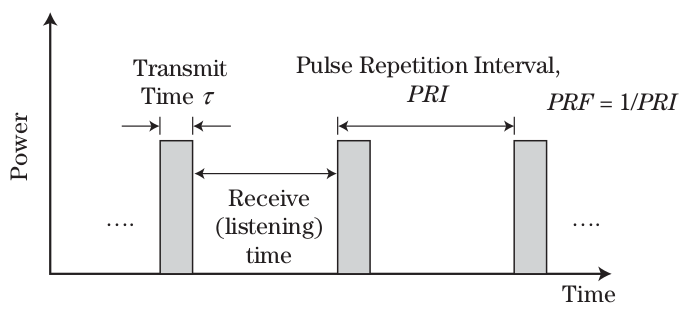
\includegraphics[width=10cm]{pulsedWaveform}
 \caption{Forma de onda de un radar pulsado \cite{Richards2010}.}
 \label{fig:pulsedWaveform}
\end{figure}


\subsection{Onda continua}

Generalmente este tipo de radares utilizan una configuración biestática, implicando que el transmisor se encuentre separado del receptor, para aumentar la aislación entre las antenas. Pero, como la aislación no es perfecta, utilizan baja potencia de transmisión. Por lo tanto, sólo son utilizados en aplicaciones de rangos cortos. Aunque hay sistemas complejos de radares de onda continua como iluminadores en sistemas de control de fuego, misiles semi activos, y rastreadores, también los hay con esquemas simples, aplicados en radares de velocidad, altímetros y sensores de proximidad \cite{Richards2010}. La figura \ref{fig:continuousWaveform} muestra un ejemplo de una modulación diente de sierra.

Dado que la transmisión es continua, la determinación del tiempo de ida y vuelta, del inglés round-trip time, de la señal electromagnética (EM) transmitida, por ende la distancia del blanco iluminado, debe realizarse cambiando las características de la señal. Por ejemplo modificando su frecuencia a través del tiempo. Esta técnica de modulación en frecuencia (FM) introduce una marca de tiempo en la onda EM, permitiendo así la determinación de la distancia al blanco.

\begin{figure}[H]
 \centering
 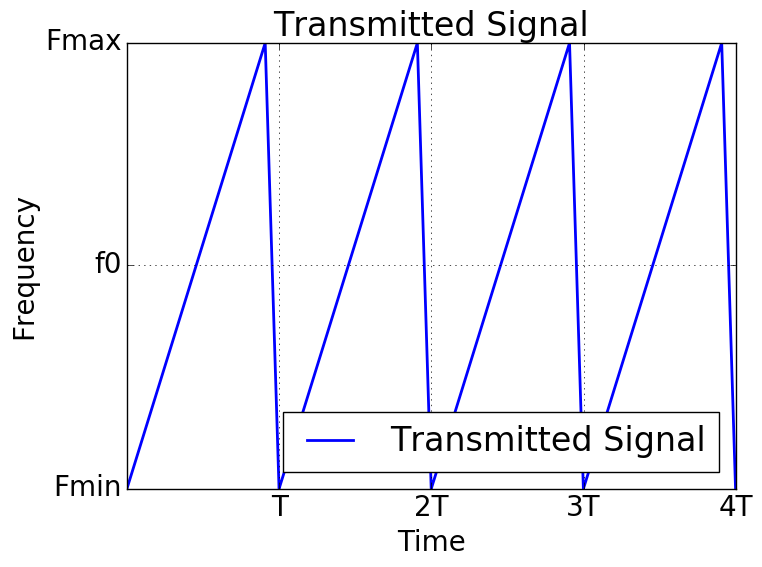
\includegraphics[width=8cm]{sawtoothSignal}
 \caption{Forma de onda de la señal transmitida por un radar FMCW.}
 \label{fig:continuousWaveform}
\end{figure}

En el presente trabajo de tesis, como se desea posicionar el cuerpo a una distancia del orden de los metros, se opta por utilizar este esquema de radares. Definiéndose de esta forma el requerimiento \ref{req:l1_radarType}.


\section{Ambigüedades en mediciones de rango} \label{sc:ambiguity}

Como la distancia a un cuerpo iluminado se mide determinando el tiempo de ida y vuelta entre la señal transmitida y el eco recibido, si dicho tiempo es mayor que el PRI, el sistema determina erróneamente dicha distancia. Este error es el llamado ambigüedad.

En la figura \ref{fig:ambiguity} se muestra un ejemplo de este efecto para un radar pulsado. Hay dos blancos, el primero a una distancia cercana y el segundo a una lejana, de tal forma, que el tiempo de ida y vuelta es mayor que el PRI. Se puede observar que el eco de la señal transmitida en el primer período del segundo blanco llega a la antena durante el tiempo de recepción del segundo período transmitido, logrando así un error en la estimación de la distancia a este blanco.

Para evitar tener ambigüedades, se debe incrementar el PRI lo suficiente para que todos los blancos estén dentro del máximo tiempo de ida y vuelta detectable.

\begin{figure}[H]
 \centering
 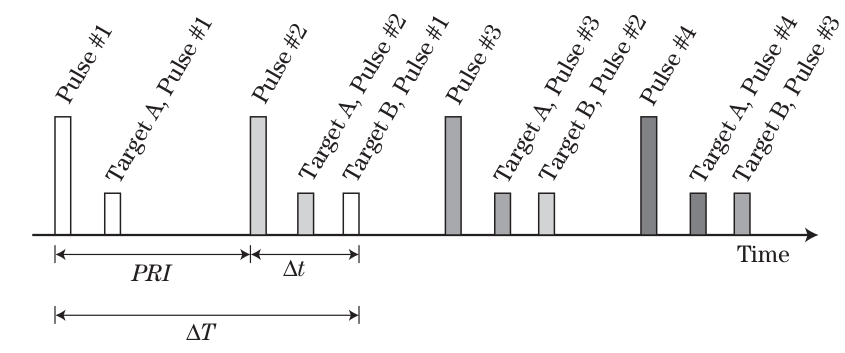
\includegraphics[width=10cm]{ambiguity}
 \caption{Ambigüedades en mediciones de rango en un radar pulsado \cite{Richards2010}.}
 \label{fig:ambiguity}
\end{figure}

En el caso de los radares FMCW, la determinación de la distancia está relacionada con la frecuencia de la señal a procesar y, dado que se transmite constantemente e independientemente de la posición en que estén los blancos iluminados, siempre habrá un solapamiento entre el pulso transmitido siguiente y la señal recibida del pulso anterior. En la figura \ref{fig:fmcwAmbiguity} se puede apreciar dicho solapamiento entre los tiempos T y T1. Como la señal a procesar es la multiplicación entre el pulso transmitido y recibido, la frecuencia recibida en el intervalo T y T1 varía a causa de la mezcla entre pulsos consecutivos, ver figura \ref{fig:modulationDelayed}.

Para evitar errores en el cálculo de la estimación en la frecuencia, se puede aplicar un retraso en la señal a procesar, evitando tomar las muestras correspondientes al solapamiento entre pulsos o se puede transmitir interrumpiendo durante un tiempo equivalente o superior al máximo tiempo de ida y vuelta de la señal admitido \cite{Varavin2007a}. Por último, para disminuir errores en dicho cálculo se aumenta la duración del tiempo T, aumentando el ancho de banda o disminuyendo la pendiente de la rampa de la señal modulada.

\begin{figure}[H]
  \centering
  \begin{subfigure}[t]{0.49\textwidth}
    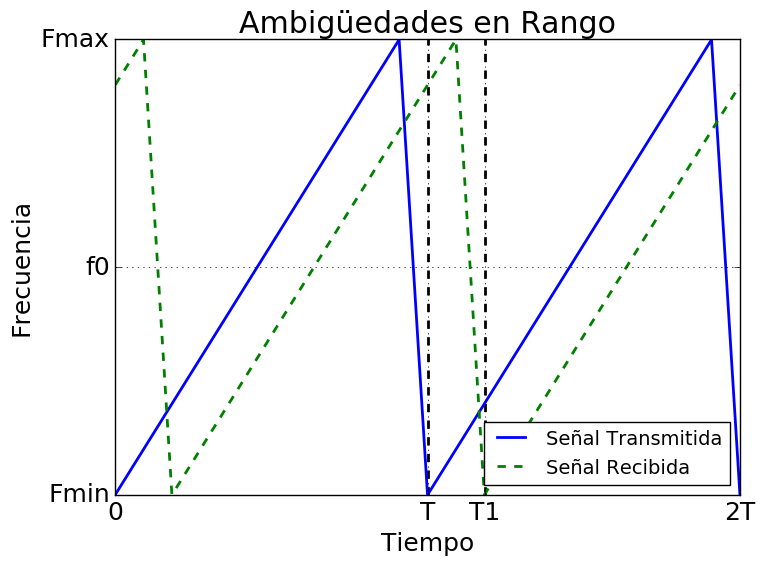
\includegraphics[width=7.5cm]{FMCWambiguity}
    \caption{Señal transmitida y recibida en función del tiempo}
    \label{fig:fmcwAmbiguity}   
  \end{subfigure}
  \begin{subfigure}[t]{0.49\textwidth}
    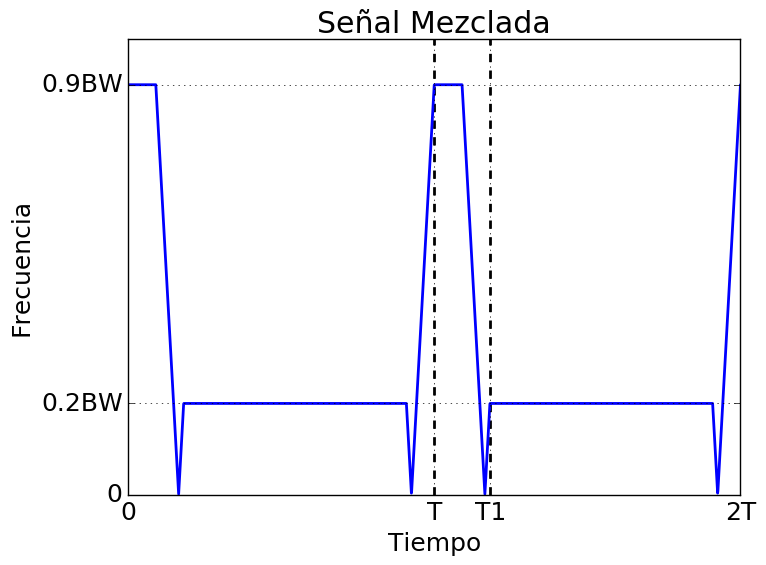
\includegraphics[width=7.5cm]{receivedFrequency}
    \caption{Frecuencia recibida de la señal a procesar.}
    \label{fig:modulationDelayed}
  \end{subfigure}             
  \caption{Ambigüedades en un radar FMCW.}
\end{figure}

\section{Antenas}

Una antena es definida como la estructura de transición entre el espacio libre y un dispositivo guía, como se muestra en la 
figura \ref{fig:antenna}. El dispositivo guía o línea de transmisión puede ser un cable coaxial o un tubo hueco (guía de 
onda), el cual es utilizado para transportar energía electromagnética desde la fuente de transmisión a la antena, o desde la 
antena al receptor. En el primer caso sería una configuración de antena transmisora y en el segundo, receptora \cite{Balanis2012}.
\begin{figure}[H]
 \centering
 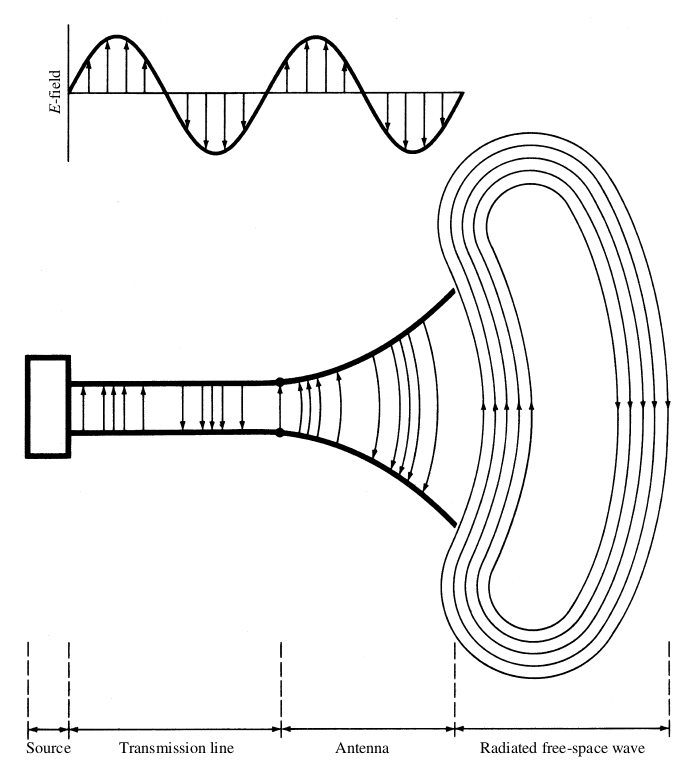
\includegraphics[width=10cm]{antenna}
 \caption{Antena como un dispositivo de transmisión \cite{Balanis2012}.}
 \label{fig:antenna}
\end{figure}

Hay una amplia variedad de antenas en la actualidad, en la tabla \ref{tab:type_antennas} se puede observar una agrupación 
simplificada.

\begin{table}[H]
  \caption{Características de cada grupo principal de antenas}
  \footnotesize
  \centering
  \begin{tabular}{l p{12.5cm}}
  \toprule
  \textbf{Tipo Antena} & \textbf{Características} \tabularnewline
  \midrule
  Cable & Son el tipo de antenas más utilizados porque se las puede en autos, edificios, barcos, sistemas aeroespaciales. Hay distintas formas de estas antenas, como monopolos, dipolos, lazos y hélices o alguna otra configuración. Los usos más comunes de los monopolos son para radios AM/FM y walkie talkies; de los dipolos son para antenas de canales de tv VHF o antena de televisión analógico; y de lazos son para receptoras de canales UHF de tv o receptores de AM \cite{Balanis2012}. \tabularnewline

  Apertura & Son el principal tipo de antenas direccionales utilizadas en frecuencias microondas. Consisten en una antena
  del tipo dipolo o Lazo junto a una estructura que guía las ondas en una dirección determinada. Este tipo de antenas son muy utilizadas en el ámbito aéreo y espacial dado que se pueden empotrar en la superficie del avión o satélite. A su vez, se los puede cubrir con un material dieléctrico para protegerlos de las condiciones ambientales \cite{Balanis2012}. \tabularnewline
  
  Microstrip & Consisten en un patch metálico sobre un sustrato. Dicho patch puede tomar distintas formas, aunque, la rectangular y circular son las más populares dada su facilidad de fabricación y por sus características de radiación, como por ejemplo la baja radiación en la polarización cruzada. Este tipo de antenas son simples, de bajo costo de fabricación, son mecánicamente robustas si se las monta en superficies rígidas y muy versátiles en términos de frecuencias de resonancia, polarización, diagramas de radiación e impedancias. Son muy utilizadas en aplicaciones aeroespaciales y celulares \cite{Balanis2012}. \tabularnewline

  Conjunto & Muchas aplicaciones requieren características de radiación que pueden no ser alcanzables con un único elemento sino que por un conjunto de elementos en una distribución eléctrica y geométrica determinada. La distribución adoptada afecta en distintos aspectos al diagrama de radiación. Algunos usos son Transmisión de canales de televisión en VHF, detección de misiles, comunicaciones satelitales \cite{Balanis2012}. \tabularnewline
  
  Reflectores & Estas antenas son utilizadas para comunicaciones a largas distancias, para transmitir y recibir señales que tienen que recorrer kilómetros. Un estilo muy común de este tipo de antenas es el reflector parabólico, el diámetro máximo construido es de $\SI{305}{\meter}$, necesario por la gran ganancia requerida para transmitir o recibir señales a miles de kilómetros. Otro tipo de reflector no tan común como la parábola es el corner reflector \cite{Balanis2012}. \tabularnewline

  Lentes & Son utilizadas principalmente para transformar energía divergente en ondas planas, de esta forma se previene  transmisión en direcciones indeseadas. Se pueden utilizar en casi las mismas aplicaciones que los reflectores parabólicos, especialmente en altas frecuencias. Para bajas frecuencias no son utilizadas dado que sus dimensiones y peso se tornan inmanejables \cite{Balanis2012}. \tabularnewline
  \bottomrule 
  \end{tabular}
  \label{tab:type_antennas}
\end{table}

Por la simplicidad de construcción, en la presente tesis se opta por utilizar el tipo de antena monopolo, de esta forma se desprende el requerimiento \ref{req:l2_antenna}. A continuación se detalla este tipo de antenas comparándolo con su contraparte, el dipolo.


\subsection{Monopolos y Dipolos}

Un monopolo es un dipolo que ha sido dividido a la mitad de su punto de alimentación central y es alimentado contra un plano de tierra, el cual actúa como un estilo de espejo eléctrico \cite{arrl2007}. La figura \ref{fig:monopoles} compara un dipolo de $\frac{\lambda}{2}$ con un monopolo de $\frac{\lambda}{4}$ de longitud. La antena imagen, para el monopolo, está representada con una línea punteada debajo del plano de tierra. La misma forma la segunda mitad de la antena, transformando funcionalmente al monopolo en un dipolo.

\begin{figure}
 \centering
 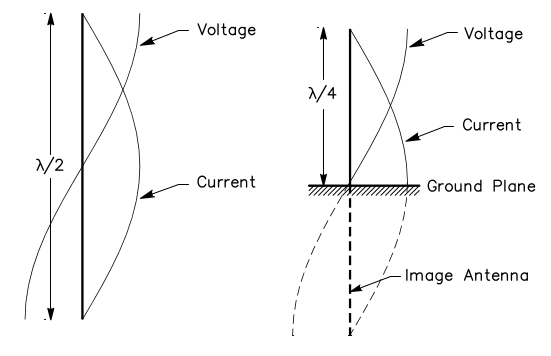
\includegraphics[width=10cm]{monopoleVsDipole}
 \caption{Un dipolo de longitud $\frac{\lambda}{2}$ y su contraparte de $\frac{\lambda}{4}$ con plano de tierra \cite{arrl2007}.}
 \label{fig:monopoles}
\end{figure}

Las cargas y corrientes en un monopolo son las mismas que la mitad superior del dipolo, aunque la tensión en sus terminales es solo la mitad, y el mismo campo eléctrico en la mitad de distancia también implica la mitad de tensión. Por lo tanto, la impedancia de entrada de un monopolo se ve disminuida a la mitad que la de su contraparte \cite{Stutzman2013},
\begin{equation}
\bm{Z}_{mono} = \dfrac{\bm{V}_{mono}}{\bm{I}_{mono}} = \dfrac{\frac{1}{2}\bm{V}_{dipolo}}{\bm{I}_{dipolo}} = \dfrac{1}{2}\bm{Z}_{dipolo}
\end{equation}
Es importante notar que la nomenclatura para valores complejos es la de utilizar letras en negrita y en itálica.

El diagrama de radiación de un monopolo sobre un plano de tierra perfecto es el mismo que el de un dipolo con las mismas dimensiones en espacio libre dado que los campos por encima del plano imagen son los mismos, ver figura \ref{fig:radingPatternDipole}. Por lo tanto, la potencia radiada por un monopolo sobre un plano de tierra perfecto es la mitad que la del dipolo en espacio libre porque la distribución de potencia es igual, pero solo sobre la mitad del espacio. Dando como resultado, el ancho del haz radiado sea la mitad que el del dipolo, llevando a que la directividad sea el doble \cite{Stutzman2013},
\begin{equation}
  D_{mono} = \dfrac{4\pi}{\Omega_{mono}} = \dfrac{4\pi}{\frac{1}{2}\Omega_{dipolo}} = 2D_{dipolo}
\end{equation}

En la práctica, un plano de tierra no puede ser infinito, aunque un plano de tierra con un radio aproximadamente igual de largo que la longitud del elemento activo resulta una solución viable. Aunque sin un sistema de tierra bien elaborado, la eficiencia del monopolo resulta drásticamente deteriorada llegando a ser menor al $\SI{50}{\percent}$ con respecto a su contraparte. Si la longitud es menor que $\frac{\lambda}{4}$ puede ser mucho peor \cite{arrl2007}.

\begin{figure}
  \centering
  \begin{subfigure}[b]{0.4\textwidth}
    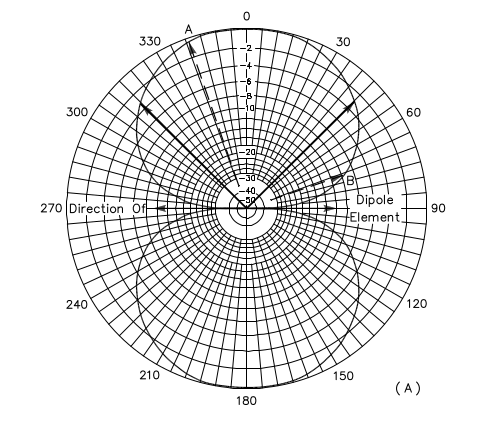
\includegraphics[width=6cm]{radiatingPatternDipole1}
    % \caption{Esquemático del modulador.}
  \end{subfigure}
  \begin{subfigure}[b]{0.4\textwidth}
    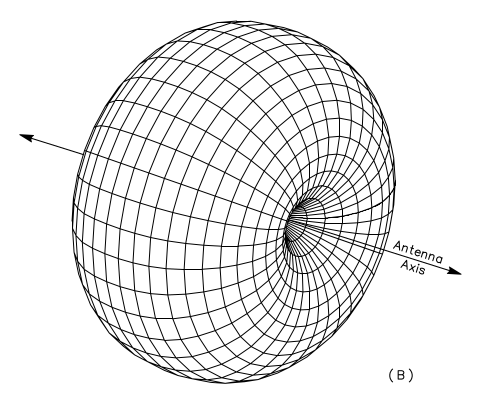
\includegraphics[width=6cm]{radiatingPatternDipole2}
    % \caption{PCB del modulador.}
  \end{subfigure}             
  \caption{Diagrama de radiación de un dipolo \cite{arrl2007}.}
  \label{fig:radingPatternDipole}
\end{figure}

La directividad de un monopolo de cuarto de longitud de onda es el doble que el un dipolo de media longitud de onda en espacio libre \cite{Stutzman2013},
\begin{equation}
  D = 2(1.64) = 3.28 = \SI{5.16}{\dB}
\end{equation}

La impedancia de entrada de un monopolo de un cuarto de longitud de onda infinitesimalmente fino resulta \cite{Stutzman2013},
\begin{equation}
  \bm{Z} = ~ (72 + j42.5) = 36 + j\SI{21.3}{\Omega}
\end{equation}

\subsection{Polarización} \label{sc:polarization}

La polarización de una onda radiada se la define como la propiedad de una onda electromagnética describiendo la variación en tiempo de la dirección y la magnitud relativa del vector del campo eléctrico; específicamente, la figura trazada en función del tiempo por la extremidad del vector en un lugar fijo en el espacio, y el sentido en que es trazado, como observado a lo largo de la dirección de propagación. Por lo tanto, la polarización es la curva trazada por la punta del vector que representa el campo eléctrico instantáneo \cite{Balanis2012}.

La polarización se puede clasificar como lineal, circular o elíptica (ver figura \ref{fig:hvPolarizations}). Si el vector que describe el campo eléctrico en un punto del espacio en función del tiempo recorre un trayecto a lo largo de una línea, se dice que el campo es linealmente polarizado (horizontalmente y/o verticalmente). En general, la figura trazada por el campo eléctrico es una elipse, nombrada polarización elíptica. La polarización lineal y circular son casos especiales de la elíptica \cite{Vita2012}.

\begin{figure}[H]
  \centering
  \begin{subfigure}[b]{0.49\textwidth}
    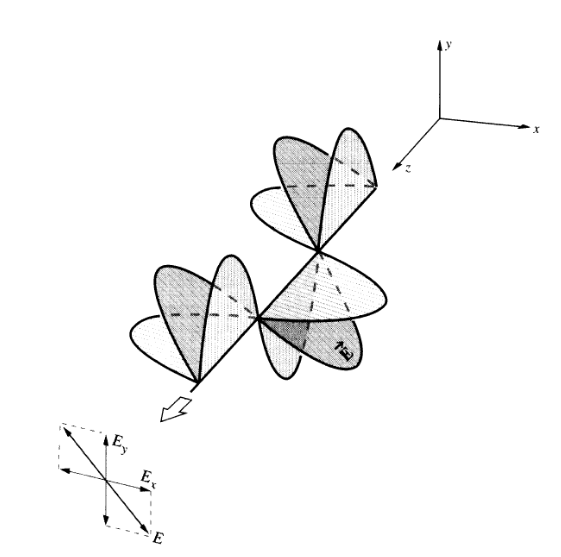
\includegraphics[width=7cm]{linearPolarization}
    \caption{Polarización lineal.}
  \end{subfigure}
  \begin{subfigure}[b]{0.49\textwidth}
    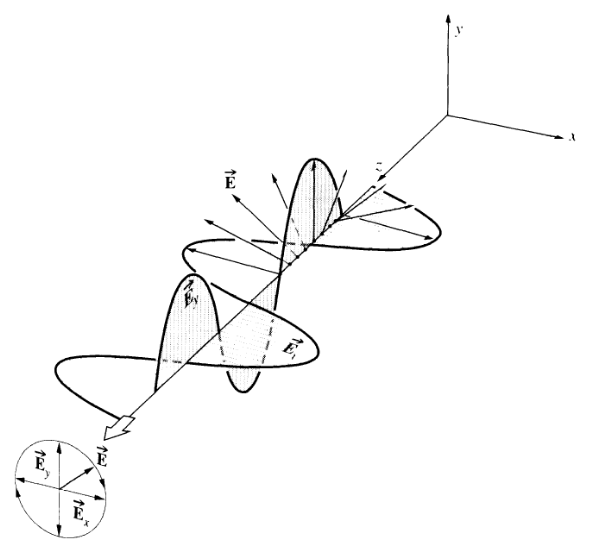
\includegraphics[width=7cm]{circularPolarization}
    \caption{Polarización circular.}
  \end{subfigure}
  \caption{Distintos tipos de polarizaciones \cite{Hecht2002}.}
  \label{fig:hvPolarizations}
\end{figure}

Para el caso de esta tesis, las antenas a construir son polarimétricas. Esto implica que poseen dos componentes, una Horizontal (H) y otra Vertical (V). Con esto se define el requerimiento \ref{req:l2_polarization}.


\section{Parámetros S} 

La sigla S deriva de la palabra dispersión. Para altas frecuencias, es conveniente describir una determinada red en términos de ondas en vez de tensiones o corrientes. Esto permite una definición más sencilla de planos de referencia. Por razones prácticas, la descripción en términos de ondas entrantes y salientes ha sido introducida. Ahora, una red de 4 polos se transforma en 2 puertos y $2n$ polos se transforman en $n$ puertos. En el caso de un número impar de polos (ej. 3 polos), un punto de referencia puede ser elegido, atribuyendo un polo igualmente a dos puertos. Por lo tanto 3 polos se convierten en 3 + 1 polo correspondiendo a 2 puertos. Como una regla general, para cantidades impares de polos, siempre se agrega un polo extra \cite{Caspers}.

\begin{figure}[H]
 \centering
 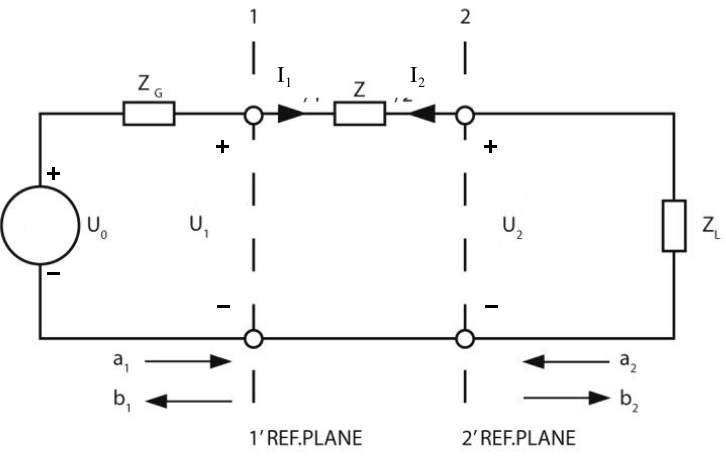
\includegraphics[width=10cm]{sParameters1}
 \caption{Ejemplo de una red de 2 puertos: circuito serie \cite{Caspers}}
 \label{fig:esquema_serie}
\end{figure}

Tomando como ejemplo una red de 2 puertos compuesta por una sola impedancia $\bm{Z}$ conectada en serie (figura \ref{fig:esquema_serie}). Las impedancias de la fuente y de la carga son $\bm{Z_G}$ y $\bm{Z_L}$ respectivamente. Si $\bm{Z}=0$ y $\bm{Z_L} = \bm{Z_G}$ (para el caso de $\bm{Z_G}$ real) la carga está adaptada. En este caso se obtiene una máxima transferencia de potencia y $\bm{U_1} = \bm{U_2} = \bm{U_0}/2$. Notar que todas las tensiones y corrientes son valores pico. Se supone que las líneas que unen los componentes poseen longitud eléctrica igual a 0. Las conexiones con una longitud eléctrica finita están dibujadas como una doble línea. A continuación se relacionará $\bm{U_0}$, $\bm{U_1}$ y $\bm{U_2}$ a $\bm{a}$ y $\bm{b}$.


\subsection{Definición de "ondas de potencia"}

Las ondas incidentes al puerto son $\textbf{a}=(\bm{a_1}, \bm{a_2}, \bm{a_3}, ..., \bm{a_n})$, las ondas salientes, o reflejadas, del puerto son $\textbf{b}=(\bm{b_1}, \bm{b_2}, \bm{b_3}, ..., \bm{b_n})$. Por definición, las corrientes incidentes son positivas y las salientes negativas. La onda $\bm{a_1}$, incidente al puerto 1, es derivada de la tensión entrante a la carga balanceada.

Para hacer que ésta definición sea consistente con la ley de la conservación de la energía. La tensión es normalizada a $\sqrt{\bm{Z_0}}$. $\bm{Z_0}$ es, en general una impedancia de referencia arbitraria, que usualmente se la utiliza como la impedancia característica de la línea (ej, $\bm{Z_0} = 50 \Omega$). Y, cuando todas las impedancias son iguales ($\bm{Z_G} = \bm{Z_L} = \bm{Z_0}$), se dice que la línea está adaptada y no hay onda reflejada. Las definiciones de $\bm{a_1}$ y $\bm{b_1}$ son
\begin{equation}
\begin{aligned}
  \bm{a_1} &= \dfrac{\bm{U_0}}{2\sqrt{\bm{Z_0}}}= \dfrac{\textrm{onda de tensión incidente (puerto 1)}}{\sqrt{\bm{Z_0}}}=\dfrac{\bm{U_1}^{inc}}{\sqrt{\bm{Z_0}}} \\
  \bm{b_1} &= \dfrac{\bm{U_1}^{refl}}{2\sqrt{\bm{Z_0}}}= \dfrac{\textrm{onda de tensión reflejada (puerto 1)}}{\sqrt{\bm{Z_0}}}
\end{aligned}
\end{equation}

Notar que \textbf{a} y \textbf{b} tienen las unidades de $\sqrt{\textrm{potencia}}$.

La potencia incidente al puerto 1, $P_{inc}$, es simplemente la potencia entregada por la fuente, mientras que la potencia saliente del puerto 1, $P_{refl}$, viene de la onda de tensión reflejada.
\begin{equation}
\begin{aligned}
  P_1^{inc} &= \dfrac{1}{2}|\bm{a_1}|^2= \dfrac{|\bm{U_1}^{inc}|^2}{2\bm{Z_0}}=\dfrac{|\bm{I_1}^{inc}|^2}{2}\bm{Z_0} \\
  P_1^{refl} &= \dfrac{1}{2}|\bm{b_1}|^2= \dfrac{|\bm{U_1}^{refl}|^2}{2\bm{Z_0}}=\dfrac{|\bm{I_1}^{refl}|^2}{2}\bm{Z_0} \\
\end{aligned}
\end{equation}

En el caso de una desadaptación de la impedancia de carga $\bm{Z_L}$, parte de la potencia será reflejada a través del puerto 2 (potencia incidente al puerto 2).
\begin{equation}
P_2^{inc}=\dfrac{1}{2}|\bm{a_2}|^2
\end{equation}

Se ha definido $\bm{a_1} = \bm{U_0}/2\sqrt{\bm{Z_0}} = \bm{U}^{inc}/\sqrt{\bm{Z_0}}$ con la onda de tensión incidente $\bm{U}^{inc}$. Como analogía se la puede definir como $\bm{a_1} = \bm{I}^{inc}\sqrt{\bm{Z_0}}$ con la onda incidente de corriente $\bm{I}^{inc}$. Utilizando ambas, se obtiene la definición general de las ondas incidentes $\bm{a_i}$ y reflejadas $\bm{b_i}$ de un puerto.
\begin{equation}
\begin{aligned}
  \bm{a_i} &= \dfrac{\bm{U_i} + \bm{I_i}\bm{Z_0}}{2\sqrt{\bm{Z_0}}} \\
  \bm{b_i} &= \dfrac{\bm{U_i} - \bm{I_i}\bm{Z_0}}{2\sqrt{\bm{Z_0}}}
\end{aligned}
\label{eq:waves}
\end{equation}

Solucionando este sistema de ecuaciones, $\bm{U_i}$ y $\bm{I_i}$ pueden ser obtenidas de $\bm{a_i}$ y $\bm{b_i}$ como
\begin{equation}
\begin{aligned}
  \bm{U_i} &= \sqrt{\bm{Z_0}}(\bm{a_i} + \bm{b_i}) = \bm{U_i}^{inc} + \bm{U_i}^{refl}\\
  \bm{I_i} &= \dfrac{1}{\sqrt{\bm{Z_0}}}(\bm{a_i} - \bm{b_i}) = \dfrac{\bm{U_i}^{refl}}{\bm{Z_0}}
\end{aligned}
\end{equation}


\subsection{La matriz de parámetros S}

La relación entre $\bm{a_i}$ y $\bm{b_i}$ (siendo $i=1..n$) puede ser escrito como un sistema de n ecuaciones lineales (siendo la variable independiente $\bm{a_i}$ y $\bm{b_i}$ la dependiente)
\begin{equation}
\begin{aligned}
  \bm{b_1} = \bm{S}_{11}\bm{a_1} + \bm{S}_{12}\bm{a_2} \\
  \bm{b_2} = \bm{S}_{21}\bm{a_1} + \bm{S}_{22}\bm{a_2}
\end{aligned}
\label{eq:s_matrix}
\end{equation}

Escrito de forma matricial: \textbf{b} = \textbf{Sa}

El significado físico de los parámetros S es:
\begin{itemize}
  \item $\bm{S}_{11}$: es el coeficiente de reflexión con la salida de la red terminada en una carga adaptada ($\bm{a_2} = 0$).
  \item $\bm{S}_{21}$: es la transmisión en directa (del puerto 1 al 2)
  \item $\bm{S}_{12}$: es la transmisión en inversa (del puerto 2 al 1)
  \item $\bm{S}_{22}$: es el coeficiente de reflexión de la salida.
\end{itemize}

Al medir todos los parámetros S de una red de n puertos, todos los puertos deben estar terminados con una carga adaptada. Utilizando las ecuaciones \ref{eq:waves} y \ref{eq:s_matrix} se obtiene el coeficiente de reflexión de una impedancia $\bm{Z_L}$ conectada a un generador de impedancia de salida $\bm{Z_0}$ (Figura \ref{fig:esquema_serie}, caso $\bm{Z_G} = \bm{Z_0}$ y $\bm{Z} = 0$)
\begin{equation}
\bm{S}_{11} = \dfrac{\bm{b_1}}{\bm{a_1}}\bigg|_{\bm{a_2}=0} = \dfrac{\bm{U_1} - \bm{I_1}\bm{Z_0}}{\bm{U_1} + \bm{I_1}\bm{Z_0}} = \dfrac{\bm{Z_L} - \bm{Z_0}}{\bm{Z_L} + \bm{Z_0}} = \bm{\Gamma}
\end{equation}


\section{Procesamiento de la señal de un radar FMCW}

Hay distintos tipos de modulaciones con las que se puede transmitir utilizando dicho tipo de radar, las cuales están resumidas a continuación.

\begin{description}

\item[Modulación diente de sierra] En esta modulación se transmite una rampa en frecuencia con respecto al tiempo y es utilizada para distancias grandes combinado con una influencia despreciable de frecuencia doppler. Si se observara un blanco estático, el eco recibido solamente posee un desplazamiento en tiempo, en cambio, si está en movimiento se genera una frecuencia doppler. Dicho efecto desplaza la frecuencia de la señal recibida incrementándola, si el blanco se mueve hacia el radar, o decrementándola, si se aleja del mismo. En esta modulación el receptor no tiene forma de separar ambas frecuencias, por lo tanto, el efecto doppler es tomado como un error en la medición. Un ejemplo es un radar de navegación marítimo \cite{Basics2015}. En \cite{Varavin2007a, Shen} se detalla el procesamiento de este tipo de modulación para un radar FMCW.

\item[Modulación Triangular] En un cambio de frecuencia de forma triangular, se pueden utilizar ambas pendientes para medir la distancia al cuerpo. Sin efecto doppler, el desplazamiento en tiempo del eco, por ende la diferencia en frecuencia es la misma tanto para la pendiente positiva como negativa. En cambio, como el efecto doppler incrementa o decrementa las frecuencias del eco, en una de las pendientes la diferencia de frecuencias se aumenta, pero para la otra decrece en la misma medida. Haciendo un análisis y comparando los resultados de cada pendiente de forma separada, se permite determinar fácilmente la diferencia en frecuencia $\Delta f$ con respecto a la frecuencia doppler $f_D$ \cite{Basics2015}. En \cite{Chang2006, Kurt2007} se detalla el procesamiento de este tipo de modulación para un radar FMCW.

\item[Modulación cuadrada o FSK] Esta modulación es utilizada para mediciones muy precisas de rango a distancias cortas. Se compara la fase de la señal recibida de las distintas frecuencias transmitidas. La mayor desventaja es que no se puede distinguir los ecos de distintos blancos iluminados y que el rango sin ambigüedades es muy chico \cite{Basics2015}.

\item[Modulación escalonada] Para detectar objetos con un mucho ruido del entorno, o clutter, para la distinción del objeto requiere alta resolución en rango. Esto se obtiene utilizando pulsos cortos y de gran ancho de banda, por lo tanto, se debe utilizar un receptor de gran ancho de banda, el cual es muy costoso. Para no utilizar un receptor de gran ancho de banda, se modula la frecuencia de forma escalonada en sucesivos pulsos, de esta forma, la resolución en rango no se ve comprometida \cite{steppedFreq}. A su vez, esta modulación se la utiliza para mediciones de interferometría y aumenta el rango de mediciones sin ambigüedades \cite{Basics2015}.

Es importante destacar que las señales que poseen una modulación del tipo rampa son llamadas chirps.

\end{description}

En esta tesis se utiliza la modulación diente de sierra dado que el radar es utilizado para realizar mediciones con blancos estáticos. De esta forma se define el requerimiento \ref{req:l2_mod}. La figura \ref{fig:sawtoothSignal} ilustra para un caso general los parámetros que definen dicha señal, los cuales son el ancho de banda de la señal transmitida ($BW$) y el período ($T$) o tiempo de repetición de dicho pulso ($PRT$).

\begin{figure}
 \centering
 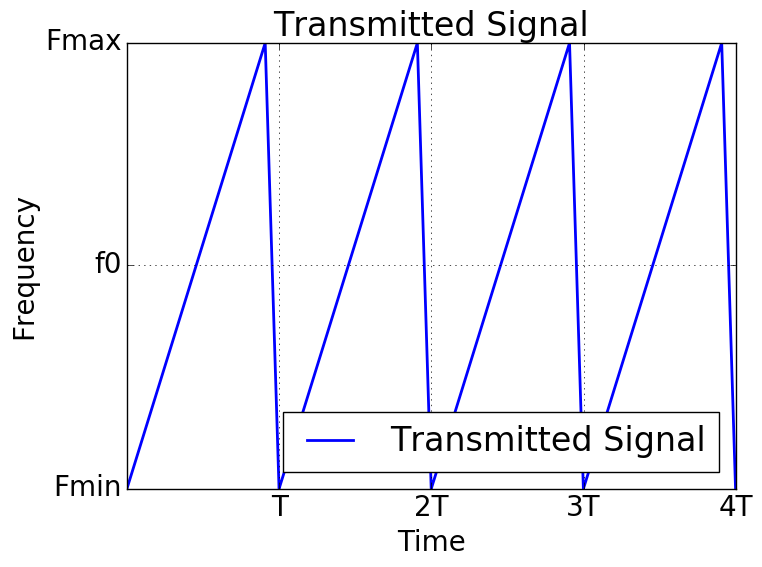
\includegraphics[width=10cm]{sawtoothSignal}
 \caption{Modulación diente de sierra de la señal a transmitir.}
 \label{fig:sawtoothSignal}
\end{figure}

Para extraer el efecto que el medio induce sobre la señal, es importante saber determinar la distancia a la cual está el cuerpo iluminado con respecto al radar. De esta forma se define el requerimiento \ref{req:l1_distance}. Para el desarrollo a continuación se asume que se está trabajando en campo lejano, con esta suposición el campo eléctrico y magnético de la onda transmitida y recibida son ortogonales a la dirección de la misma. En general, cuando se está a unas pocas longitudes de onda de distancia ya se cumple esta condición. En un monopolo se cumple a una distancia $r$ aproximadamente igual a $\lambda/ 6$ \cite{Richards2009}.


\subsection{Determinación de distancia}

Para determinar la distancia de un cuerpo iluminado se mide el tiempo de ida y vuelta de la señal transmitida. En la figura \ref{fig:roundTripTime} se muestra la modulación de una chirp transmitida por el radar y el eco recibido, producido por dicho blanco a una distancia $R$. Se puede observar que el tiempo de ida y vuelta de la señal está marcado como $\tau$.

\begin{figure}
 \centering
 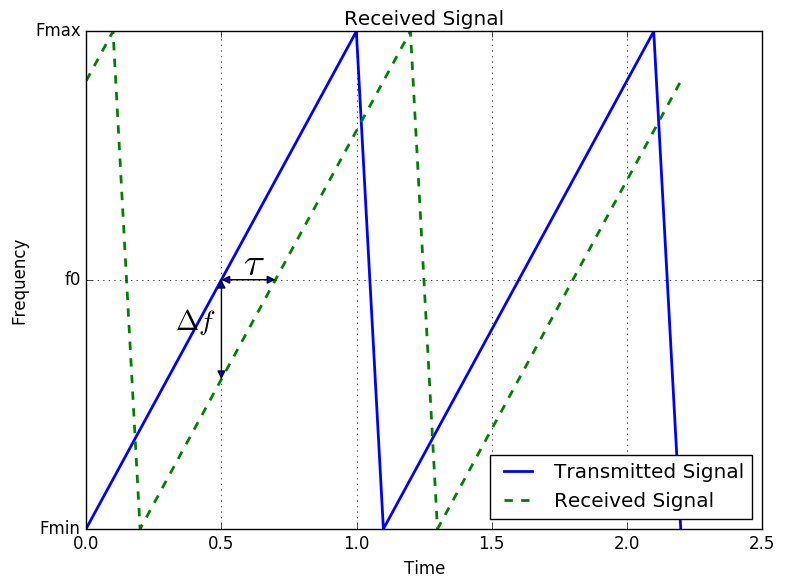
\includegraphics[width=10cm]{round-tripTime}
 \caption{Modulación diente de sierra de la señal a transmitir.}
 \label{fig:roundTripTime}
\end{figure}

La relación entre el tiempo de ida y vuelta $\tau$ y la distancia es,
\begin{equation}\label{eq:relDist}
  \tau = \dfrac{2R\sqrt{\varepsilon_r}}{c}
\end{equation}
donde $\varepsilon_r$ es la permitividad relativa del medio.

Este tipo de radares utiliza la relación entre la diferencia de tiempo $\tau$ y la diferencia en frecuencia, $\Delta f$, entre las señales transmitidas y recibidas,
\begin{equation}\label{eq:relFreqDist}
  \tau = \dfrac{T\Delta f}{B}
\end{equation}
donde $B$ es el ancho de banda de la señal y $T$ es el tiempo en que es barrido el BW, desde la frecuencia mínima a la máxima, sin contar el tiempo que tarda el generador en volver de la frecuencia máxima a la mínima. Por lo tanto utilizando las ecuaciones \ref{eq:relDist} y \ref{eq:relFreqDist} se puede determinar la distancia $R$ a partir de la señal recibida,
\begin{equation}\label{eq:receivedDist}
  R = \dfrac{T\Delta fc}{2B\varepsilon_r}
\end{equation}

Para determinar la resolución en distancia, se debe tener en cuenta que la misma está relacionada con la resolución espectral de la señal recibida. Asumiendo $T >> T_d$, el ancho de banda a $\SI{-3}{\dB}$ con respecto a su pico es igual a $1/T$ \cite{Brooker2005}. Es importante destacar que dicho valor es igual a la distancia entre las frecuencias nulas, dado que el espectro se corresponde a una sinc.
\begin{equation}\label{eq:resolutionDistance}
  \Delta R = \dfrac{c}{2B\sqrt{\varepsilon_r}}
\end{equation}

Se puede apreciar que la resolución en distancia obtenida, ecuación \ref{eq:resolutionDistance}, no depende ni del período ($T$) de la señal transmitida ni de su frecuencia central ($f_0$), solamente de su ancho de banda ($B$). Hay que tener en cuenta que las alinelidades de la señal modulada degradan la resolución obtenida, y la misma depende del ancho de banda, por lo tanto, la mayor resolución se obtiene tomando en cuenta ambos efectos \cite{Brooker2005}.

Como la distancia al cuerpo se determina midiendo la frecuencia de la señal recibida, o en su defecto el pico de la sinc en frecuencia, se pueden agregar ceros al final de la señal para aumentar la resolución de la FFT. Dicho proceso es llamado zero padding \cite{Oppenheim1990}.
\begin{equation}\label{eq:resolutionDistance2}
  \Delta R = \dfrac{c}{2B\sqrt{\varepsilon_r}p}
\end{equation}

Siendo $p$ la relación entre la frecuencia de muestreo $f$ de la señal y la cantidad de muestras $n$ utilizada para realizar la FFT.
\begin{equation}
  p = \frac{f}{n}
\end{equation}


\subsection{Determinación de la relación de fase}

Para determinar la fase del cuerpo iluminado es necesario realizar un análisis de la fase de la señal recibida. La figura \ref{fig:phaseSystem} muestra el recorrido de la señal, en particular centrando en el análisis que se está realizando.
\begin{figure}[htb]
 \centering
 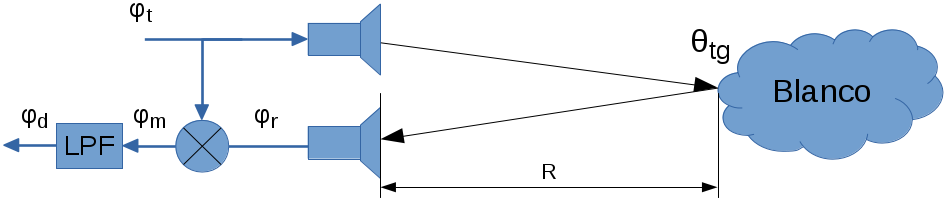
\includegraphics[width=10cm]{phaseMeasurement}
 \caption{Análisis de fase del sistema completo.}
 \label{fig:phaseSystem}
\end{figure}

La ecuación que define la modulación de cada período del pulso se encuentra descripta a continuación,
\begin{equation}
  f(t) = f_0 + \dfrac{B}{T}(t-\dfrac{T}{2}),\quad 0 \le t < T
  \label{eq:signalFrequency}
\end{equation}

donde $c$ es la velocidad de la luz, $\varepsilon_r$ es la constante dieléctrica del medio \cite{Brennan2014a} y $T$ es el tiempo en que es barrido el BW, desde la frecuencia mínima a la máxima, sin contar el tiempo que tarda el generador en volver de la frecuencia máxima a la mínima. Dado que la fase de una señal es la integral de su frecuencia sumada a una constante, se obtiene la fase instantánea transmitida a partir de la ecuación \ref{eq:signalFrequency},
\begin{equation}
  \varphi_t(t) = 2\pi f_0t + \dfrac{2\pi B}{2T}(t^2-Tt) + \phi_0,\quad 0 \le t < T
  \label{eq:signalFrequency2}
\end{equation}

El eco recibido por un objeto puntual en una distancia $R$ y desfasando la señal en $\theta$ llega al radar con la fase,
\begin{equation}
  \varphi_r(t) = w_0(t-\tau) + \dfrac{2\pi B}{2T}((t - \tau)^2-T(t - \tau)) + \theta + \phi_0,\quad 0 \le t < T
  \label{eq:signalFrequency3}
\end{equation}

donde $\tau$ es el tiempo ida y vuelta de la señal entre el transmisor y receptor del radar obtenido de la ecuación \ref{eq:relDist}.

Luego, en el mezclador, la señal recibida se la multiplica con la transmitida, por identidad trigonométrica, se obtiene
\begin{equation}
  x_m(t) = \dfrac{A_tA_r}{2}(\cos(\varphi_t(t)+\varphi_r(t)) + \cos(\varphi_t(t)- \varphi_r(r)))
  \label{eq:signalFrequency4}
\end{equation}

Donde $A_r$ es la amplitud de la señal recibida, la cual es modificada por el ida y vuelta del medio y por el blanco donde se genera el eco de la señal.

Que, luego del filtro pasa bajos, el primer término de la ecuación \ref{eq:signalFrequency4}, el cual posee una frecuencia de $2w_0$, resulta completamente atenuado, quedando solamente el término con la resta de fases,
\begin{equation}
  x_d(t) = \dfrac{A_tA_r}{2}\cos(w_0\tau + \dfrac{2\pi B\tau}{T}(t - \dfrac{T}{2}) - \dfrac{2\pi B\tau^2}{2T} - \theta)
  \label{eq:signalFrequency5}
\end{equation}

Es importante notar que la fase inicial de transmisión se elimina, por lo tanto no importa cual es la fase inicial de cada pulso
transmitido ni su variación entre pulsos. Para determinar la frecuencia de la señal recibida se deriva la ecuación \ref{eq:signalFrequency5}, 
\begin{equation}\label{eq:beatFreq}
  w_d = \dfrac{2\pi B\tau}{T} \rightarrow f_d = \dfrac{B\tau}{T}
\end{equation}

Se puede observar que el resultado obtenido es coherente con el resultado de la ecuación \ref{eq:relFreqDist}, el cual muestra la relación entre el round-trip time y la diferencia en frecuencia entre la señal transmitida y recibida.

Del resultado de la ecuación \ref{eq:signalFrequency5} se observa que la fase de la señal recibida está compuesta por cuatro términos.
\begin{itemize}
  \item $w_0\tau$ es el término utilizado para determinar distancias con alta precisión en blancos conocidos \cite{Brennan2014a}.
  \item $\dfrac{2\pi B\tau}{T}(t - \dfrac{T}{2})$ es un término de fase lineal con el tiempo que representa la frecuencia de la señal.
  \item $\dfrac{2\pi B\tau^2}{2T}$ es un offset en la señal, usualmente pequeño.
  \item $\theta$ es el término de fase originada por el blanco donde incidió la señal transmitida por el radar.
\end{itemize}

Para obtener el término de la fase originada por el blanco, $\theta$, primero se calcula la FFT de la señal recibida y se mide la fase del pico de la sinc, $\varphi_d$. Si no se realiza ninguna rotación a la señal en el momento del cálculo, el valor de $t$ correspondiente al segundo término es igual a 0. Luego, se debe restar dicho valor a la fase de los primeros tres términos correspondientes a la la distancia medida, 
\begin{equation}\label{eq:phaseMeasurement}
  \theta =  w_0\tau - \pi B\tau - \dfrac{\pi B\tau^2}{T} - \varphi_d  = \dfrac{2w_0R}{c} - \dfrac{2\pi BR}{c} - \dfrac{4\pi BR^2}{Tc^2} - \varphi_d
\end{equation}

Para utilizar la ecuación anterior, es fundamental que la diferencia de fase entre dos pulsos consecutivos en frecuencia sea menor que $2\pi$. Para ello, se realiza zero padding en la señal previo al cálculo de la FFT.

% Si se quisiera utilizar $w_0\tau$ para calcular la distancia, primero se tiene que hacer zero padding en la señal (para calcular la frecuencia de round trip time) de manera tal que la diferencia de fase entre dos pulsos consecutivos en frecuencia (que estan totalmente relacionados a $\Delta R$) sea menor que $2\pi$. Con esto, el $\Delta R$ al que está relacionado el pico de frecuencia entre dichos pulsos se puede determinar univocamente. La relación entre la fase y dicha distancia es $\Delta R = \frac{\lambda\phi}{4\pi}$, está dividido por 4 porque la distancia medida es el doble a la distancia entre el radar y el obteto iluminado.

% Sabiendo que la relación entre la distancia y la frecuencia medida, expresada en \ref{eq:beatFreq}, la máxima diferencia de distancia en que puede estar el objeto iluminado es igual a $\Delta R = \frac{c}{2B\sqrt{\varepsilon_r}}$, $\Delta f_d = \frac{1}{T}$ dado que es la resolución el frecuencia. Por lo tanto, la diferencia de fase es.

% \begin{equation}
%   \Delta(\omega_0\tau) = \dfrac{\omega_02\Delta R \sqrt{\varepsilon_r}}{c} = \dfrac{\omega_c}{B} = \dfrac{2\pi f_0}{B}
% \end{equation}


% \mynote{however, the phase indicated by an FFT is that at the start of the sample, at t = 0. It is therefore necessary to rotate the deramped (time-domain) waveform so that the centre of the waveform aligns with the start of the sample, t = 0, prior to FFT processing \cite{Brennan2014a}}

% \mynote{For processing convenience, it would be highly desirable if
% the phase relating to a point target located at the centre of each range bin is normalised to zero. This can be achieved by weighting the FFT-processed deramped waveform by a reference array equal to the phase conjugate of the expected phase at the centre of each range bin}

% \mynote{Seleccionar una función de ventana no es una tarea simple. Cada función de ventana tiene sus propias características y aptitud para diferentes aplicaciones. Para elegir una función de ventana, usted debe calcular el contenido de la frecuencia de la señal.
% Si la señal contiene componentes de frecuencia de fuerte interferencia alejados de la frecuencia de interés, elija una ventana con un rango alto de caída del lóbulo lateral.
% Si la señal contiene fuertes señales de interferencia cerca de la frecuencia de interés, elija una función de ventana con un nivel bajo de lóbulo lateral máximo.
% Si la frecuencia de interés contiene dos o más señales muy cerca una de la otra, la resolución espectral es importante. En este caso, es mejor elegir una ventana con un lóbulo principal muy estrecho.
% Si la precisión de la amplitud de un solo componente de frecuencia es más importante que la ubicación exacta del componente en un contenedor de frecuencia determinado, elija una ventana con un lóbulo principal amplio.
% Si el espectro de la señal es más bien plano o de banda ancha en el contenido de frecuencia, utilice la ventana uniforme o ninguna ventana.
% En general, la ventana Hanning (Hann) es satisfactoria en el 95\% de los casos. Tiene buena resolución de frecuencia y menor fuga espectral. Si no conoce la naturaleza de la señal, pero desea aplicar una ventana, comience con la ventana de Hann.
% http://www.ni.com/white-paper/4844/es/}


% \mynote{el mismo libro \cite{Richards2009} tiene una buena definicion con un buen grafico de polarización.}

\subsection{Determinación de la relación de amplitud}


Para determinar la ganancia del blanco, se debe realizar un análisis de potencia en todo el sistema, el cual se ilustra en la figura  \ref{fig:powerAnalysis}. Se puede observar que la señal transmitida posee atenuaciones por el medio en que la señal es transmitida y recibida, el blanco, las ganancias de transmisión y recepción de las antenas, el mezclador del receptor y el filtro pasa bajos. 

\begin{figure}
 \centering
 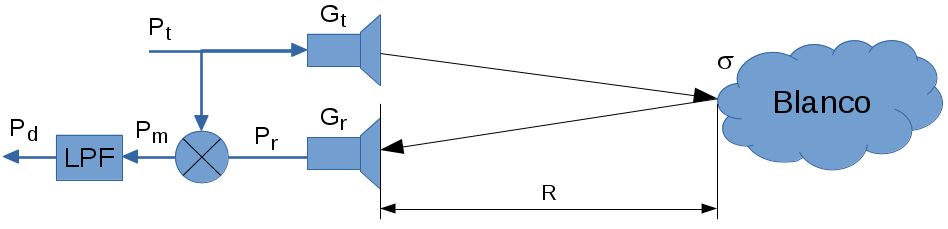
\includegraphics[width=10cm]{targetMeasurement}
 \caption{Análisis de la potencia de la señal.}
 \label{fig:powerAnalysis}
\end{figure}

Cuando el radar transmite una potencia $P_t$ y si fuese un radiador isotrópico, la densidad de potencia incidente en un cuerpo a una distancia R es igual a $P_t$ dividido el área unitaria,
\begin{equation}
  p_i = \dfrac{P_t}{4\pi R^2} \,[\si{Wm^{-2}}]
\end{equation}

Cuando el radiador no es isotrópico y el radar utiliza una antena que concentra la potencia en una dirección en particular, la densidad de potencia incidente resulta
\begin{equation}
  p_i = \dfrac{P_tG_t}{4\pi R^2} \,[\si{Wm^{-2}}]
\end{equation}

donde $G_t$ es la ganancia de la antena transmisora, definida como la relación entre densidades de potencia en la dirección en particular con respecto a un radiador isotrópico \cite{Richards2009}. Ahora, si se asume que el blanco posee un Radar Cross Section (RCS) igual a $\sigma \,[\si{m^2}]$, la potencia disponible para ser nuevamente irradiada en el blanco es 
\begin{equation}
  p_\sigma = p_i\sigma = \dfrac{P_tG_t\sigma}{4\pi R^2} \,[\si{W}]
\end{equation}

A su vez, si se asume que el blanco irradia isotrópicamente, la densidad de potencia en la antena receptora es 
\begin{equation} \label{eq:receivedDensity}
  p_r = \dfrac{P_tG_t\sigma}{(4\pi)^2 R^4} \,[\si{Wm^{-2}}]
\end{equation}

La potencia recibida es la densidad multiplicada por la apertura de la antena $A_r$, que también tiene dimensiones de área. La cual está relacionada con la ganancia de recepción por 
\begin{equation} \label{eq:receptionGain}
  G_r = \dfrac{4\pi A_r}{\lambda^2}
\end{equation}

Por lo tanto, utilizando la ecuación \ref{eq:receivedDensity} con \ref{eq:receptionGain}, la potencia recibida $P_r$ por el radar es igual a
\begin{equation}
  P_r = \dfrac{P_tG_tG_r\lambda^2\sigma}{(4\pi)^3 R^4} \,[\si{W}]
\end{equation}

La señal recibida es mezclada con la señal transmita y, si se asume un mezclador ideal, la potencia de salida $P_m$ es la multiplicación de las potencias de entrada, por lo tanto
\begin{equation}
  P_m = P_tP_r = \dfrac{P_t^2G_tG_r\lambda^2\sigma}{(4\pi)^3 R^4} \,[\si{W}]
\end{equation}

Por último, la señal mezclada es filtrada eliminando los componentes de alta frecuencia, asumiendo un filtro ideal y observando que en la ecuación \ref{eq:signalFrequency4} se elimina el término correspondiente a la suma de frecuencias, se puede deducir que la potencia de salida es la mitad que la de entrada.
\begin{equation} \label{eq:derampedPower}
  P_d = \dfrac{P_m}{2} = \dfrac{P_t^2G_tG_r\lambda^2\sigma}{2(4\pi)^3 R^4} \,[\si{W}]
\end{equation}

Ahora que se posee la relación entre la potencia de la señal a procesar y la ganancia del blanco (ecuación \ref{eq:derampedPower}), se puede determinar la relación de amplitud
\begin{equation}
  \sigma = \dfrac{2P_d(4\pi)^3 R^4}{P_t^2G_tG_r\lambda^2} \,[\si{m^2}]
\end{equation}


\section{Resumen}

En este capítulo se introdujeron los conceptos básicos sobre los dos grandes grupos de radares, los cuales son pulsados o continuos y se menciona la problemática de ambigüedades en rango asociada a cada uno de ellos. En la problemática a resolver se opta por la utilización de radares continuos a causa de la cercanía entre el blanco y el radar.

Con respecto a las antenas, se menciona una lista de los distintos tipos con descripciones y usos. Se detallan los monopolos y dipolos dado que es el tipo de antena utilizado por su simpleza de construcción. A su vez, se introduce el concepto de parámetros S y de polarización vertical y horizontal dado que las antenas utilizadas son del tipo polarimétricas y se las caracteriza midiendo dichos parámetros.

Por último, se resumen los principales tipos de modulaciones utilizados en un radar continuo detallando el diente de sierra. Asimismo, se describe el desarrollo matemático para la determinación de la distancia entre el objeto y el radar. Esto es necesario dado que la misma es utilizada para poder determinar tanto la fase como la ganancia que el blanco induce sobre la señal. Dichas perturbaciones son las variables que determinan los parámetros de dispersión.

\begin{description}

\item[Distancia entre el blanco y el radar]
Dicha variable está determinada por
\begin{equation}
  R = \dfrac{T\Delta fc}{2B\varepsilon_r} \pm \dfrac{c}{2B\sqrt{\varepsilon_r}p}
\end{equation}
donde $c$ es la velocidad de la luz, $\varepsilon_r$ es la permitividad relativa del medio, $B$ es el ancho de banda de la señal, $\Delta f$ es la diferencia de frecuencia instantánea entre la señal transmitida y recibida, $T$ es el tiempo en que es barrido el BW, desde la frecuencia mínima a la máxima y $p$ es la relación entre la frecuencia de muestreo de la señal y la cantidad de muestras utilizada para realizar la FFT.

\item[Atenuación que el blanco induce sobre la señal]
Dicha variable está determinada por
\begin{equation}
  \sigma = \dfrac{2P_d(4\pi)^3 R^4}{P_t^2G_tG_r\lambda^2}
\end{equation}
donde $P_d$ es la potencia de la señal a procesar, $P_t$ es la potencia transmitida del radar, $G_t$ es la ganancia de la antena transmisora y $G_r$ es la ganancia de la antena receptora.

\item[Desfase que el blanco induce sobre la señal]
Dicha variable está determinada por
\begin{equation}
  \theta = \dfrac{4\pi f_0R}{c} - \dfrac{2\pi BR}{c} - \dfrac{4\pi BR^2}{Tc^2} - \varphi_d
\end{equation}
donde $f_0$ es la frecuencia central de la señal transmitida y $\varphi_d$ es la fase de de la señal recibida.

Para utilizar la ecuación anterior, es fundamental que la diferencia de fase entre dos pulsos consecutivos en frecuencia sea menor que $2\pi$. Para ello, se realiza zero padding en la señal previo al cálculo de la FFT.
\end{description}
\chapter{Desarrollo del Hardware} \label{ch:development}

% **************************** Define Graphics Path **************************
\ifpdf
    \graphicspath{{Chapter3/Figs/Raster/}{Chapter3/Figs/PDF/}{Chapter3/Figs/}}
\else
    \graphicspath{{Chapter3/Figs/Vector/}{Chapter3/Figs/}}
\fi

En este capítulo se presenta el desarrollo físico del dispositivo en función de las bases teóricas y los requerimientos definidos en el capítulo previo. El mismo se encuentra dividido en dos secciones. En la primera se explica que criterios fueron tomados en cuenta y que componentes se utilizaron para la construcción de cada sección del radar. En la segunda, se muestran las mediciones realizadas para caracterizar los distintos módulos que lo integran.


\section{Construcción}

En la figura \ref{fig:radarDiagram} se puede observar un diagrama en bloques mostrando los distintos módulos que integran el radar construido. Las siguientes secciones del capítulo explican cada uno de estos módulos por separado, salvo el procesador que se explicará en el capítulo \ref{sc:radarProcessor}.
\begin{figure}
 \centering
 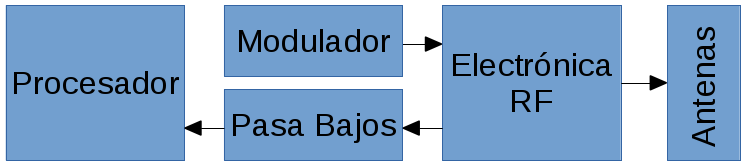
\includegraphics[width=10cm]{radarScheme}
 \caption{Diagrama en bloques básico del radar FMCW a construir.}
 \label{fig:radarDiagram}
\end{figure}


\subsection{Modulador}

Como se mencionó en la sección \ref{sc:ambiguity}, para evitar ambigüedades en la determinación del rango de medición la duración de la chirp transmitida debe ser mayor que el tiempo de ida y vuelta al blanco más alejado detectable por el radar. Como se desea una distancia máxima igual a $\SI{20}{\meter}$ (ver requerimiento \ref{req:l0}), siguiendo la relación de la ecuación \ref{eq:relDist}, se puede determinar el mínimo valor admitido de dicho período.
\begin{equation}
  \tau = \dfrac{2R\sqrt{\varepsilon_r}}{c} \approx \SI{133.43}{\nano\second}
\end{equation}

A su vez, en la sección \ref{sc:ambiguity} también se mencionó que para disminuir errores en el cálculo de la estimación en la frecuencia, se busca que el período de la señal transmitida sea al menos dos órdenes mayor que el máximo tiempo de ida y vuelta. Por lo tanto, el mínimo período resulta igual a $\SI{13.343}{\mu\second}$. De esta forma se desprende el requerimiento \ref{req:l2_pulseT}.

Las especificaciones del modulador utilizado en todos los ensayos están definidos en la tabla \ref{tab:modulatorsSpecification}. Las mismas definen los requerimientos \ref{req:l2_mod} y \ref{req:l2_dutyCycle}.

\begin{table}[htb]
  \caption{Especificaciones del modulador.}
  \centering
  \label{tab:modulatorsSpecification}
  \begin{tabular}{l c}
  \toprule
  \textbf{Característica} & \textbf{Especificación} \tabularnewline
  \midrule

  Modulación & Triangular, Senoidal \tabularnewline

  $V_{pp}$ & $\SI{5}{V}$ \tabularnewline

  Período & $\SI{14.8}{\milli\second}$ \tabularnewline

  Duty Cycle & $\SIrange[range-phrase = \rightarrow]{0.05}{99.995}{\percent}$ \tabularnewline

  \bottomrule
  \end{tabular}
\end{table}

El circuito integrado utilizado para armar el modulador, con las especificaciones mencionadas en la tabla \ref{tab:modulatorsSpecification}, es el XR-2206. Se trata de un generador de señales y su hoja de datos está especificada en \cite{Generator1972}. Dentro del mismo están los circuitos de una señal triangular, cuadrada, diente de sierra, entre otros.

En este trabajo se diseñó un circuito que, según la posición de jumpers, se modifica el tipo de señal generada. De esta forma se cumple el requerimiento \ref{req:l2_mod}. La imagen \ref{fig:schematicModulator} muestra el esquemático del circuito y la figura \ref{fig:pcbModulator} muestra el pcb. Se puede observar que el circuito posee dos llaves, $S_1$ y $S_2$, el primero es para elegir la señal de salida, sinusoidal o triangular y el segundo es para modificar el ciclo de trabajo. Para el caso sin ciclo de trabajo, la frecuencia de salida depende de la siguiente ecuación,
\begin{equation}
  f = \dfrac{1}{R_1C}
\end{equation}
en cambio, para el otro caso, 
\begin{equation}
  f = \dfrac{2}{(R_1 + R_2)C}
\end{equation}
y el ciclo de trabajo es
\begin{equation}
  \Delta T = \dfrac{R_1}{R_1 + R_2}
\end{equation}
\begin{figure}[H]
  \centering
  \begin{subfigure}[b]{0.65\textwidth}
    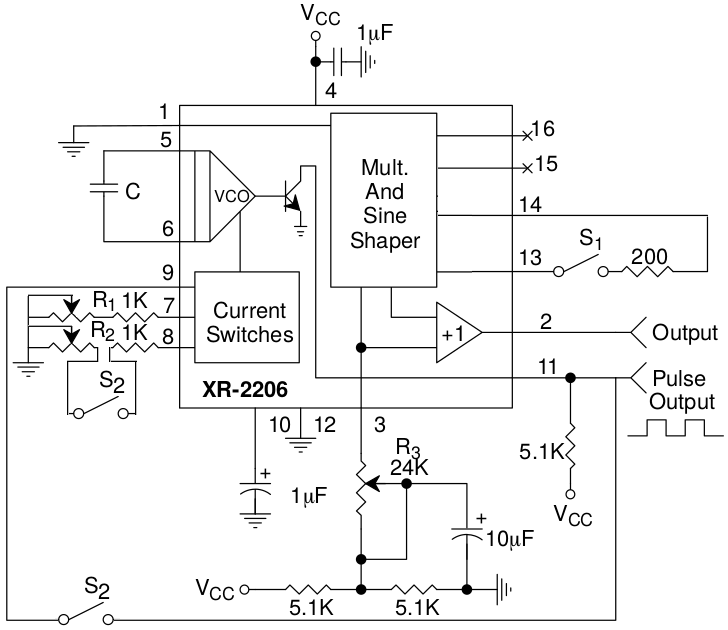
\includegraphics[width=9.5cm]{modulator}
    \caption{Esquemático del modulador.}
    \label{fig:schematicModulator} 
  \end{subfigure}

  \begin{subfigure}[b]{0.65\textwidth}
    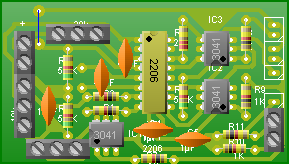
\includegraphics[width=9.5cm]{pcbModulator}
    \caption{PCB del modulador.}
    \label{fig:pcbModulator}
  \end{subfigure}

  \begin{subfigure}[b]{0.65\textwidth}
    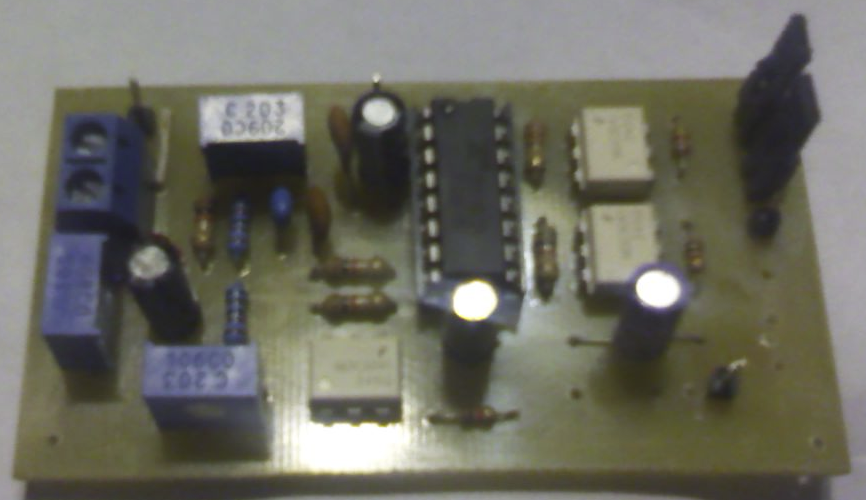
\includegraphics[width=9.5cm]{realModulator}
    \caption{Circuito construido del modulador.}
  \end{subfigure}
  \caption{Distintas etapas en la construcción del Modulador del radar.}
\end{figure}


\subsection{Electrónica de RF}

Se decidió utilizar como base la electrónica RF de un radar FMCW de banda S de baja potencia diseñado por el Instituto de Tecnología de Massachusetts (MIT). La cual posee una potencia de transmisión igual a $\SI{12}{\dBm}$. Con esto se define el requerimiento \ref{req:l2_txPower}.

La cadena está compuesta por un generador controlado por tensión (VCO), atenuadores, divisores de potencia, amplificadores y un mezclador, ver figura \ref{fig:rfElectronics}. A continuación se describen las principales características de cada uno de los componentes mencionados.

\begin{figure}[htb]
  \centering
  \begin{subfigure}{\textwidth}
    \centering
    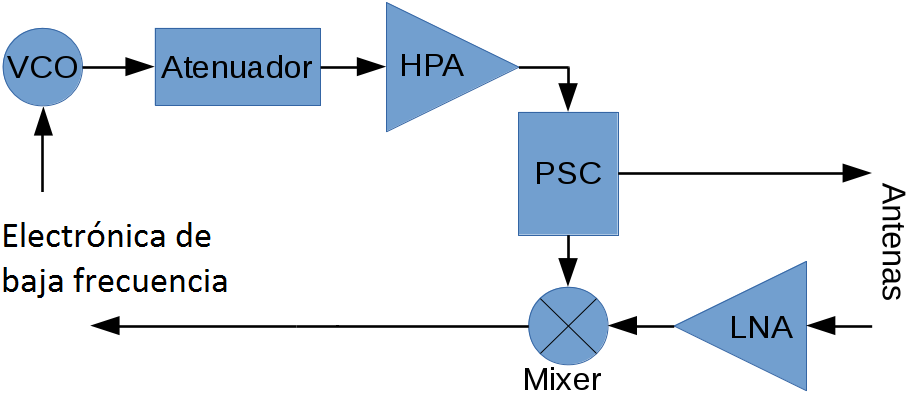
\includegraphics[width=10cm]{rfElectronics}
    \caption{Circuito esquemático}
  \end{subfigure}

  \begin{subfigure}{\textwidth}
    \centering
    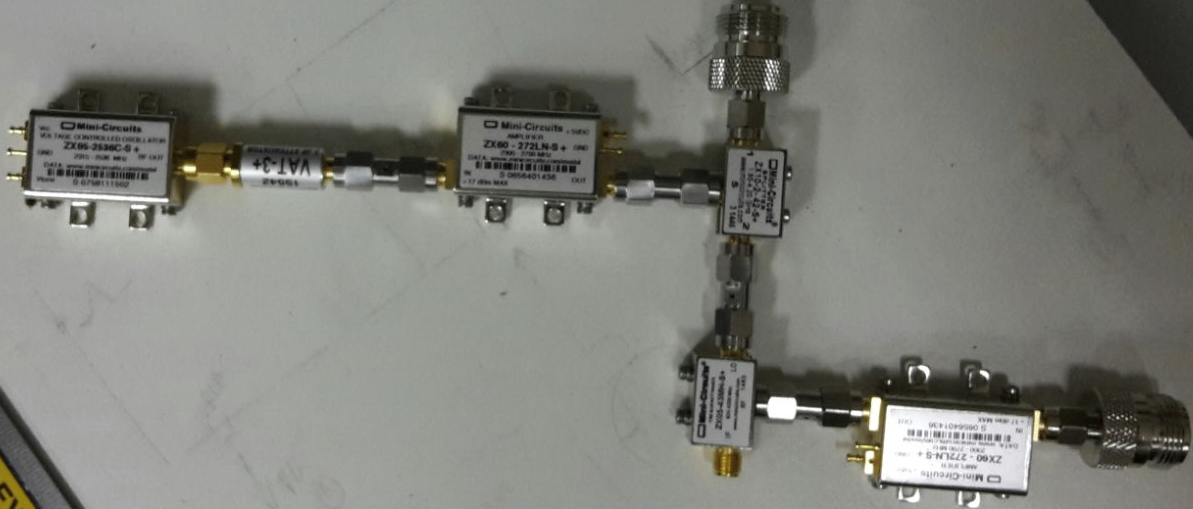
\includegraphics[width=10cm]{rfElectronics2}
    \caption{Electrónica de RF armada.}
  \end{subfigure}
  \caption{Distintas etapas en la construcción de la electrónica de RF.}
  \label{fig:rfElectronics}
\end{figure}

\begin{description}
  \item[VCO] El código de dicho componente es ZX95-2536C \cite{VCOMiniCircuits}. La frecuencia de la señal transmitida depende de la tensión de entrada, dicha dependencia puede observarse en la figura \ref{fig:freqVsVoltage}. La potencia transmitida es de $\SI{6.2}{\dBm}$ cuando la tensión de alimentación es de $\SI{5}{V}$. La frecuencia central de trabajo es igual a $\SI{2450}{\MHz}$ y posee un ancho de banda de transmisión máximo igual a $\SI{300}{\MHz}$. De esta forma se definen los requerimientos \ref{req:l2_f0} y \ref{req:l2_bw}.
  \begin{figure}[H]
   \centering
   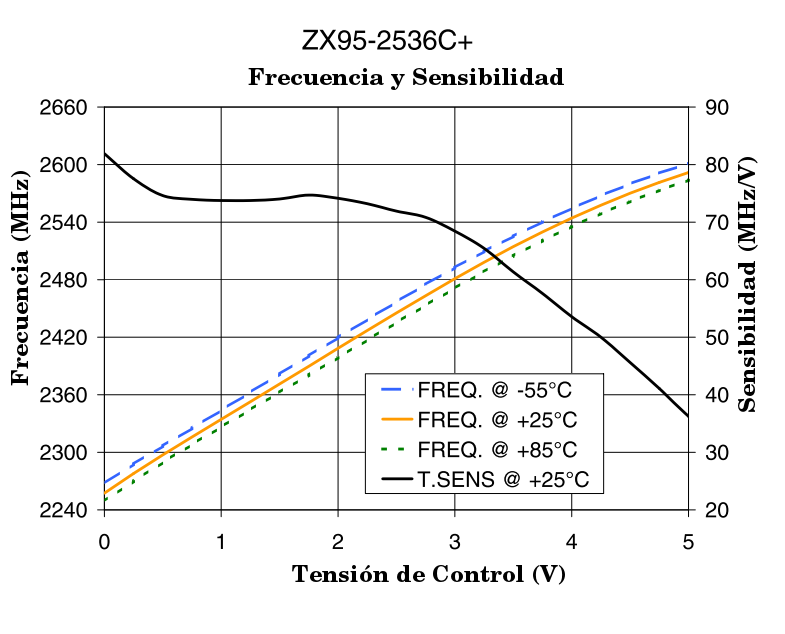
\includegraphics[width=10cm]{frequencyVsVoltage}
   \caption{Frecuencia generada en función de la tensión de control \cite{VCOMiniCircuits}.}
   \label{fig:freqVsVoltage}
  \end{figure}
  
  \item[Atenuador] El código de dicho componente es VAT-3 \cite{AttMiniCircuits}. En la frecuencia de trabajo del VCO, la señal es atenuada en $\SI{3.2}{\deci\bel}$. El mismo es utilizado para proteger al generador ante cualquier señal reflejada por desadaptaciones o por mal conexionado del instrumental.

  \item[Divisor de potencia] El código de dicho componente es ZX10-2-42 \cite{PSCMiniCircuits}. El mismo posee una pérdida por inserción desde el puerto central a los individuales igual a $\SI{3.26}{\dB}$ en una frecuencia de $\SI{2460}{\MHz}$. La figura \ref{fig:insertionLoss} muestra dicha pérdida en función de la frecuencia de trabajo.

  \begin{figure}[H]
   \centering
   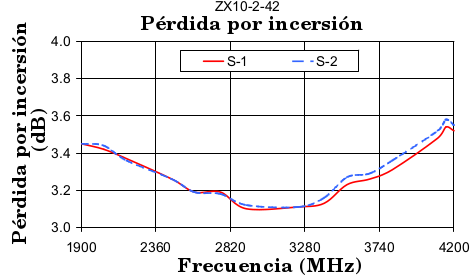
\includegraphics[width=10cm]{insertionLoss}
   \caption{Pérdida de inserción en el divisor de potencia \cite{PSCMiniCircuits}.}
   \label{fig:insertionLoss}
  \end{figure}

  \item[Amplificador] El código de dicho componente es ZX60-272LN \cite{LNAMiniCircuits}. Según la hoja de datos, el mismo posee una ganancia igual a $\SI{14}{\deci\bel}$ para la frecuencia central de trabajo del VCO.

  \item[Mezclador] El código de dicho componente es ZX05-43MH \cite{mixerMiniCircuits}. Según la hoja de datos, el mismo posee una pérdida por conversión igual a $\SI{5.5}{\deci\bel}$ para la frecuencia central de trabajo del VCO.

\end{description}


\subsection{Antenas}

Las antenas escogidas son del tipo apertura dado que se requiere cierta direccionalidad. A su vez, se decide utilizar una para transmitir y otra para recibir. Por cada cavidad hay dos monopolos distribuidos de forma ortogonal entre sí para poder transmitir y recibir en ambas polarizaciones, horizontal (H) y vertical (V). De esta forma se definen los requerimientos \ref{req:l2_antQuantity}, \ref{req:l2_antenna} y \ref{req:l2_polarization}. Los atributos a definir son la altura de la pesca, la distancia de la misma a la pared de la cavidad, la longitud y diámetro del caño. Los mismos dependen de la frecuencia de trabajo y el modo en que se desee trabajar.

\begin{figure}
 \centering
 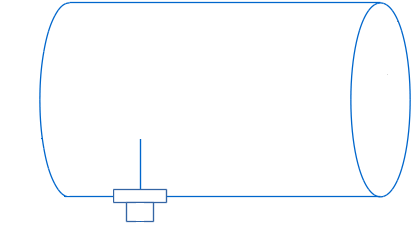
\includegraphics[width=8cm]{antennas}
 \caption{Dimensiones de una guía de onda de medio tubo.}
 \label{fig:antennas}
\end{figure}

Cada modo de resonancia es definido por una frecuencia de corte inferior, el cual no podría existir a frecuencias inferiores. El modo dominante es el que posee la menor frecuencia de corte posible. Para este tipo de guías de ondas es el TE$_{11}$. En este modo no hay campo eléctrico en la dirección de la propagación de la onda y define la relación entre el radio de la antena, $R$, y la frecuencia de corte \cite{circularWaveguides}.
\begin{equation} \label{eq:freqInf}
  f_c = \dfrac{\num{1.8412}}{2\pi R} c
\end{equation}

La longitud de onda dentro de la guía es mayor a la de la señal en espacio libre y responde a la siguiente ecuación,
\begin{equation} \label{eq:lambdaInGuide}
\lambda_g = \begin{cases} \dfrac{\lambda}{\sqrt{1 - (\dfrac{f_c}{f})^2}}, & \mbox{donde } f > f_c \\ \infty, & \mbox{donde } f = f_c \end{cases}
\end{equation}

Se debe elegir el tamaño de la guía de forma tal que el ancho de banda de operación entre completamente dentro de dicho modo de de resonancia, por lo tanto la máxima frecuencia de trabajo debe ser menor a la frecuencia de corte de TE$_{21}$ \cite{circularWaveguides},
\begin{equation} \label{eq:freqSup}
  f_{csup} = \dfrac{\num{3.0542}c}{2\pi R}
\end{equation}

\begin{description}
  \item[Altura de la pesca] Este atributo se corresponde con el requerimiento \ref{req:l2_pescaLength} y se define como la cuarta parte de la longitud de onda de la señal transmitida en espacio libre. En este caso se utiliza la frecuencia central de trabajo.

  \begin{equation}
  WireLength = \dfrac{\lambda}{4}
  \end{equation}

Dado que la frecuencia de trabajo utilizada es igual a $\SI{2450}{\MHz}$, la longitud de la pesca resulta aproximadamente igual a $\SI{3}{\centi\meter}$.

  \item[Longitud y diámetro de la guía de onda circular] Estos atributos se corresponden con el requerimiento \ref{req:l2_cavity}. Como se mencionó previamente, las frecuencias de cortes inferiores de cada modo de resonancia depende del diámetro de la guía de ondas, por lo tanto el ancho de banda de cada modo se encuentra determinado por las mismas. Y como se desea que las frecuencias de trabajo, $\SI{2300}{\MHz} - \SI{2600}{\MHz}$, entren dentro del modo dominante, el diámetro máximo y mínimo admisible es de,
  \begin{equation}
  \SI{7.64}{\centi\meter} < D < \SI{11.2}{\centi\meter}
  \end{equation}

  El resultado anterior fue obtenido siguiendo las ecuaciones \ref{eq:freqInf} y \ref{eq:freqSup}. La antena que se consiguió posee una longitud igual a $\SI{15}{\centi\meter}$ y un diámetro igual a $\SI{10}{\centi\meter}$, por lo tanto, el ancho de banda admisible del modo dominante es de $\SI{1157.5}{\MHz}$ con una frecuencia central de $\SI{2335.75}{\MHz}$.

  \item[Distancia monopolo a la pared de la guía de onda] Este atributo se corresponde con el requerimiento \ref{req:l2_cavityDistance}. Dado que la guía de onda es cilíndrica y que el monopolo transmite omnidireccionalmente en el plano perpendicular al mismo \cite{arrl2007}, parte de la onda se transmite hacia el frente de la guía pero otra parte hacia el fondo, la misma se refleja con la pared metálica volviendo al punto de origen con dirección del frente de la antena.

  Para que la interferencia de ondas sea constructiva, es necesario que el eco posea la misma fase que la señal a transmitir. Se logra el efecto deseado si la separación entre el monopolo y la pared es de $\frac{\lambda}{4}$, dado que el eco en un medio metálico implica un desfase de $\SI{180}{\degree}$. Siguiendo la ecuación \ref{eq:lambdaInGuide}, y dado que la frecuencia central de trabajo es de $\SI{2450}{\MHz}$, la longitud de onda dentro de la guía de onda es igual a $\SI{17.56}{\centi\meter}$, por lo tanto la distancia resultante es $\SI{4.39}{\centi\meter}$.

\end{description}

\subsection{Pasa Bajos}

El circuito pasa bajos del receptor, utilizado para filtrar todas las frecuencias salvo las pertenecientes al rango de trabajo del radar, es el sallen-key \cite{Unwin2003}. Este circuito, ilustrado en la figura \ref{fig:lowPassCircuit}, consta de tres etapas. La primera es un amplificador no inversor y las siguientes son pasa bajos de segundo orden con una frecuencia de corte del orden de $\SI{20}{\kHz}$, conformando un circuito de cuarto orden con una frecuencia de corte igual a los $\SI{20}{\kHz}$, definiéndose así el requerimiento \ref{req:l2_filter}. Dicho valor surge de que la señal, luego de ser filtrada, se recibe en la computadora a través del jack del micrófono, el cual posee una frecuencia de muestreo de $\SI{40}{\kHz}$. Por lo tanto, para cumplir con el teorema de nyquist, si se desea evitar el aliasing en la señal, la frecuencia máxima no puede superar $\SI{20}{\kHz}$.

Cabe destacar que, como el radar trabaja con tensiones de $\SI{12}{\volt}$ y $\SI{5}{\volt}$, los amplificadores están alimentados con la tensión de mayor denominación y las resistencias conectadas a sus pines inversores con la tensión de menor denominación.

\begin{figure}
 \centering
 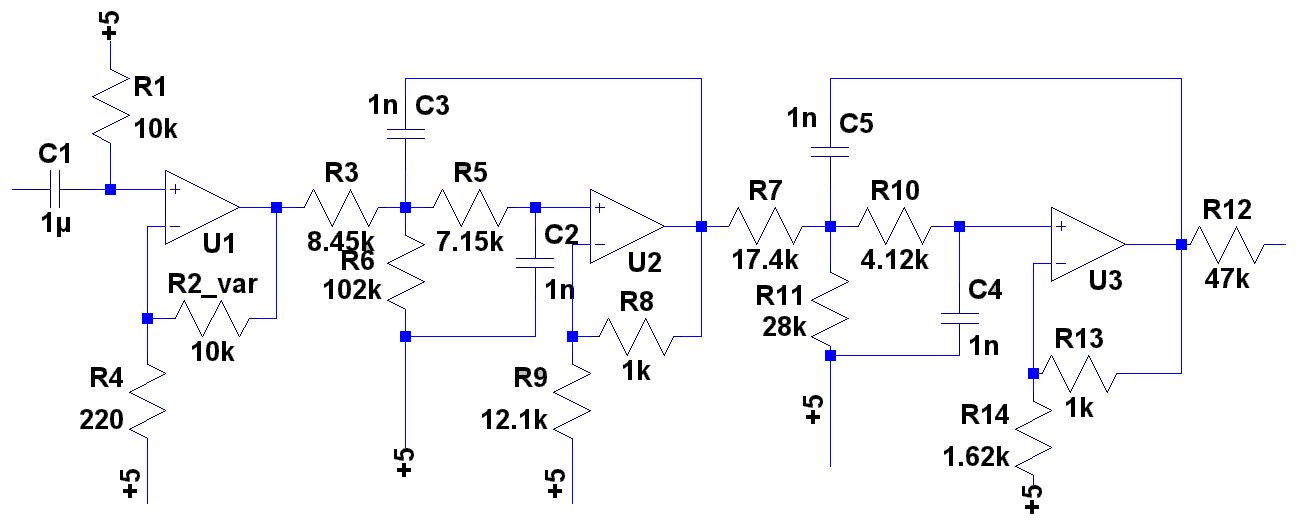
\includegraphics[width=15cm]{lowPassBand}
 \caption{Circuito pasa bajos y amplificador de señal.}
 \label{fig:lowPassCircuit}
\end{figure}

La entrada al circuito amplificador posee un capacitor en serie para eliminar el offset de la señal de entrada y una resistencia conectada a los $\SI{5}{\volt}$ estableciendo el offset común. La existencia del capacitor en serie a la señal resulta en un circuito pasa altos, con una frecuencia de corte inferior igual a
\begin{equation}\label{eq:fcInf}
  fc = \dfrac{1}{2\pi R_1 C_1} = \SI{7.23}{\Hz}
\end{equation}

La ecuación \ref{eq:gainAmplifier} es la transferencia de este circuito para cuando se considera despreciable la influencia del capacitor serie sobre la señal.
\begin{equation}\label{eq:gainAmplifier}
  Av = 1 + \dfrac{R_2}{R_4}
\end{equation}

Las siguientes etapas fueron caracterizadas utilizando las ecuaciones que definen al filtro sallen-key, listadas en la referencia \cite{Unwin2003}. Pero, como dichos circuitos no son exactamente iguales por la existencia de las resistencias $R_6$ y $R_{11}$ de la figura \ref{fig:lowPassCircuit}, dichas ecuaciones no pueden ser utilizadas directamente. Si se realiza un corte en cada etapa, como se muestra en la figura \ref{fig:genericSallen}, para calcular el equivalente de thevenin, se obtiene el circuito mostrado en la figura \ref{fig:genericSallen2}.

\begin{figure}
  \centering
  \begin{subfigure}{0.4\textwidth}
    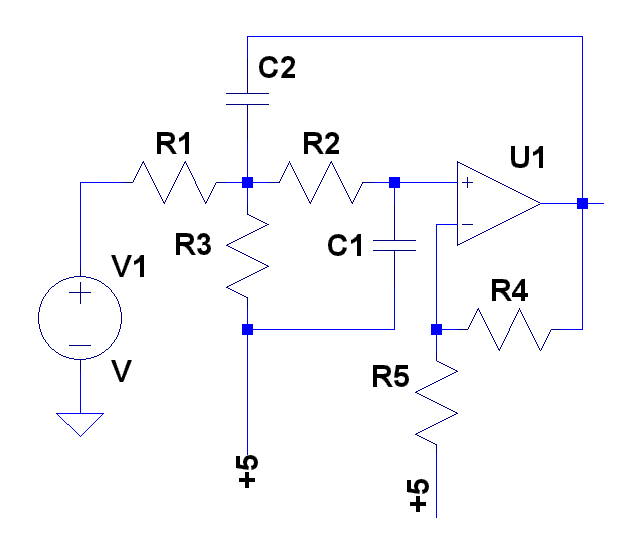
\includegraphics[width=6cm]{genericSallenKey}
    \caption{Etapa generica del circuito pasa bajo del radar}
    \label{fig:genericSallen}   
  \end{subfigure}
  {\color{blue}\LARGE$\Rightarrow$}
  \begin{subfigure}{0.4\textwidth}
    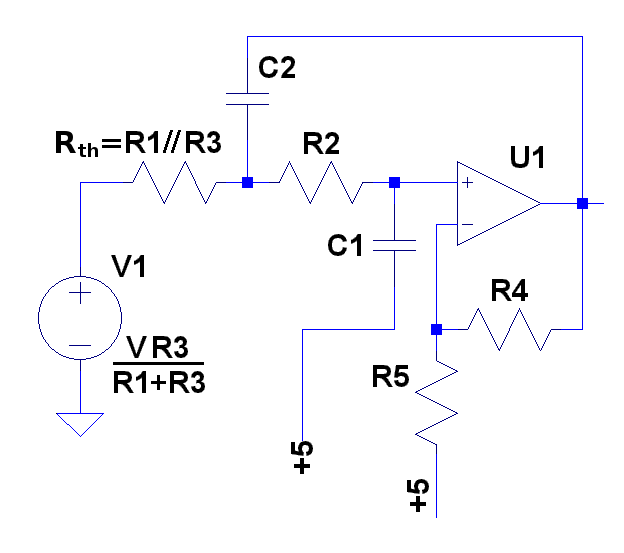
\includegraphics[width=6cm]{genericSallenKey2}
    \caption{Equivalente del circuito pasa bajos del radar}
    \label{fig:genericSallen2}
  \end{subfigure}             
  \caption{Equivalente filtro Sallen-key}
\end{figure}
Manteniendo la nomenclatura de los componentes mostrados en la figura \ref{fig:genericSallen2}, las ecuaciones para calcular la ganancia a bajas frecuencias, la frecuencia de corte y el Q de cada etapa son \ref{eq:gainLowPass}, \ref{eq:f0LowPass} y \ref{eq:qLowPass} respectivamente.
\begin{equation}\label{eq:gainLowPass}
  Av = 1 + \dfrac{R_4}{R_5}
\end{equation}
\begin{equation}\label{eq:f0LowPass}
  f_0 = \dfrac{1}{2\pi\sqrt{R_{th}R_2C_1C_2}}
\end{equation}
\begin{equation}\label{eq:qLowPass}
  Q = \dfrac{\sqrt{R_{th}R_2C_1C_2}}{R_{th}C_1 + R_2C_1 + \dfrac{R_{th}C_2R_4}{R_5}}
\end{equation}

La tabla \ref{tab:lowPassProperties} resume la ganancia y frecuencias de corte y Q de cada etapa.

\begin{table}[htb]
  \caption{Propiedades de las etapas del filtro del receptor.}
  \centering
  \label{tab:lowPassProperties}
  \begin{tabular}{l c c c}
  \toprule
  \textbf{Etapa} & \textbf{Ganancia} & \textbf{Frecuencia Corte} & \textbf{Q} \tabularnewline
   & [veces] & [Hz] & \tabularnewline
  \midrule
  Primera & 1 - 46,45 & - & - \tabularnewline

  segunda & 1,08 & 21306 & 0,52 \tabularnewline

  tercera & 1,62 & 23935 & 0,8 \tabularnewline

  \bottomrule
  \end{tabular}
\end{table}

Las imágenes de la figura \ref{fig:lowPassFilterCircuit} muestran el PCB y el circuito pasa bajos armado.
\begin{figure}[H]
  \centering
  \begin{subfigure}[b]{0.47\textwidth}
    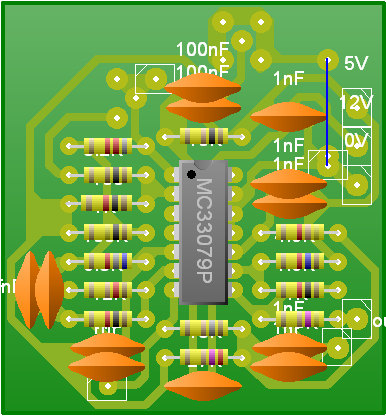
\includegraphics[width=7cm]{pcbLPF}
    \caption{PCB del filtro pasa bajos.}
  \end{subfigure}
  \begin{subfigure}[b]{0.47\textwidth}
    \includegraphics[width=7cm]{lowPassFilter}
    \caption{Circuito construido del filtro pasa bajos.}
  \end{subfigure}
  \caption{Distintas etapas en la construcción del filtro pasa bajos del radar.}
  \label{fig:lowPassFilterCircuit}
\end{figure}


\subsection{Procesador}

Dado que el procesador es software, se lo detallará junto al simulador en el capítulo \ref{ch:softwareDevelopment}.

\subsection{Gabinete}

El hecho de querer montar en un futuro al radar en un dron introduce ciertos requerimientos de volumen y peso que afectan en la decisión del gabinete a utilizar, como el que no debe pesar más de $\SI{1}{\kg}$. Dado que se requiere que sea lo más liviano posible y en un volumen determinado, se optó por utilizar plástico como material. El compuesto del mismo es poliestireno de alto impacto y es fabricado con la técnica de termoformado. El peso final del radar resulta ser de $\SI{600}{\gram}$ cumpliéndose el requerimiento \ref{req:l2_weight}.

Como habrán otros componentes electrónicos que pueden afectar al funcionamiento del radar por interferencia electromagnéticas (EMI), se debe metalizar el gabinete. Una de las posibles estrategias es la del metalizado al vacío, aunque dicho proceso quedará como trabajo futuro.

La figura \ref{fig:radar3D} muestran la modelización del radar completo, como se vería el interior como el exterior del mismo.
\begin{figure}[H]
 \centering
 \begin{subfigure}[t]{0.49\textwidth}
    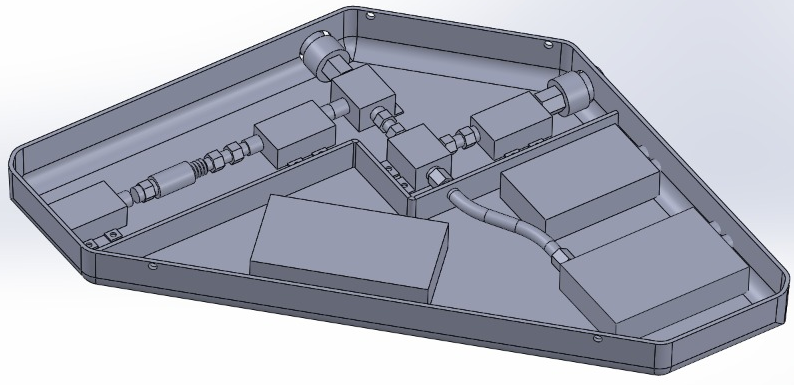
\includegraphics[width=7.5cm]{radar3D}
  \end{subfigure}
  \begin{subfigure}[t]{0.49\textwidth}
    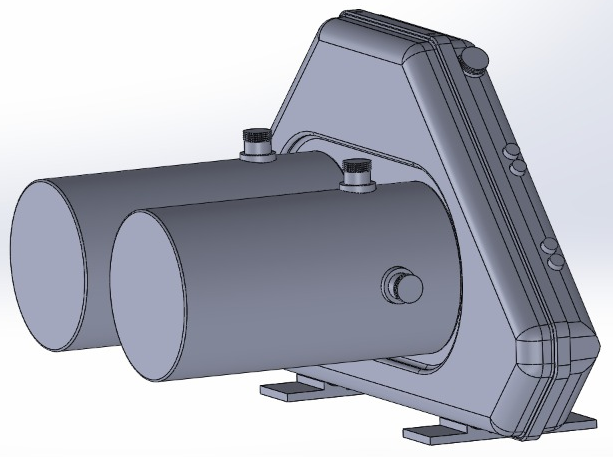
\includegraphics[width=7.5cm]{completeRadar}
  \end{subfigure}
 \caption{Modelo del gabinete interna y exterma.}
 \label{fig:radar3D}
\end{figure}

La figura \ref{fig:completeRadar} muestra tanto el interior del gabinete armado con la distribución de los componentes dentro del mismo como el radar de perfil.

\begin{figure}[H]
 \centering
 \begin{subfigure}[t]{0.8\textwidth}
    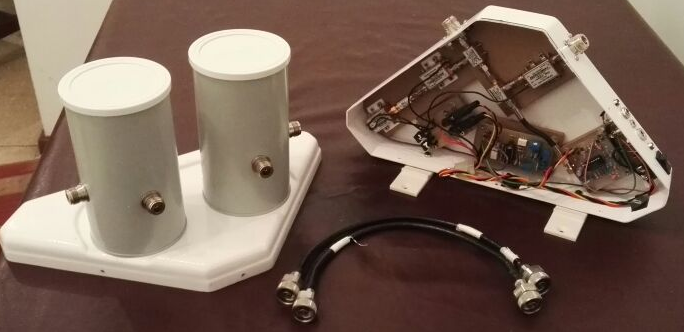
\includegraphics[width=12cm]{openedRuiltRadar}
  \end{subfigure}

  \begin{subfigure}[t]{0.5\textwidth}
    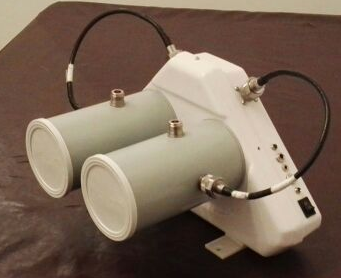
\includegraphics[width=7.5cm]{completeBuiltRadar}
  \end{subfigure}
 \caption{Modelo del gabinete interna y externa.}
 \label{fig:completeRadar}
\end{figure}


\section{Mediciones de funcionamiento}

En esta sección se muestran distintas mediciones sobre diversos módulos del radar para caracterizarlo.
Los instrumentos utilizados son
\begin{itemize}
  \item Analizador de espectros: Rhode \& Schwartz ESU 40 \cite{spectrumAnalyzer}.
  \item Analizador de redes Vectorial (VNA): Keysight Technologies N9923A FieldFox RF.
Vector Network Analyzer \cite{VNA}.
  \item Osciloscopio: Goodwill, GOS-653G
  \item Contador: GoodWill, GUC-2020
  \item Generador de señales: Topward, FG-8140
\end{itemize}

\subsection{Transferencia, filtro pasa bajos}

Para la medición de la función de transferencia del filtro se utilizó un generador de señales, un osciloscopio y un contador. Al primero se lo conectó a la entrada del circuito. Al resto del instrumental se lo conectó tanto a la entrada como a la salida del mismo. La figura \ref{fig:lowPassFilterConnections} muestra el banco de trabajo utilizado para realizar la medición.

\begin{figure}[H]
 \centering
 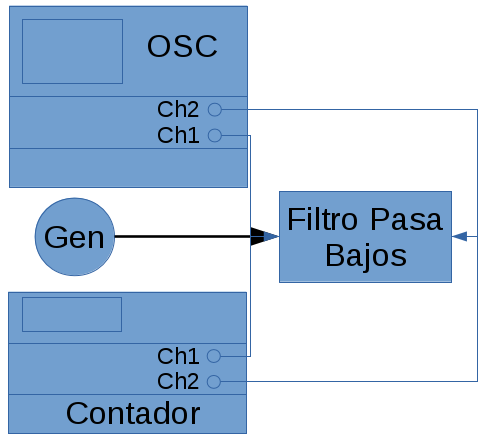
\includegraphics[width=6cm]{lowPassFilterTransferenceWorkbench}
 \caption{Banco de medición, transferencia del filtro pasa bajos.}
 \label{fig:lowPassFilterConnections}
\end{figure}

Durante el ensayo se midió tanto la tensión de entrada como la de salida con el osciloscopio a medida que se fue variando la frecuencia del generador para determinar la ganancia del circuito. A su vez, con el contador se determinó el desfase entre ambas señales midiendo el intervalo de tiempo entre los flancos ascendentes de cada una. La tabla \ref{tab:lowPassFilterTransference} y la figura \ref{fig:lowPassFilterTransference} muestran los resultados obtenidos.

La incertidumbre de las mediciones de tensiones medidas es del $\SI{3}{\percent}$. Por lo tanto la incertidumbre de la ganancia es del $\SI{6}{\percent}$. En cambio, la incertidumbre del intervalo de tiempo y el de la frecuencia ronda el $\SI{1}{\percent}$ dado que el instrumento fue configurado para disminuir la incertidumbre asociada a la medición. Por lo tanto la incertidumbre del desfase es del $\SI{2}{\percent}$. La tabla \ref{tab:lowPassFilterTransference} y la figura \ref{fig:lowPassFilterTransference} muestran los resultados obtenidos.

En la figura \ref{fig:lowPassFilterTransference} se muestran dos curvas, en rojo la ganancia y en azul la fase en función de la frecuencia. Se puede observar que el ancho de banda del circuito es aproximadamente de $\SI{20}{\kHz}$ con una frecuencia de corte inferior igual a $\SI{10}{\Hz}$. Es importante notar que la misma es plana hasta una frecuencia de $\SI{10}{\kHz}$. En cambio, observando el desfase del circuito, el mismo es igual a $\SI{0}{\degree}$ en un rango de frecuencias de $\SI{30}{\Hz}$ a $\SI{2}{\kHz}$. Si la señal recibida se encuentra en otros valores de frecuencias, habría que substraer el efecto de este subsistema sobre la misma para eliminar el error sistemático. De esta forma se verifica el requerimiento \ref{req:l2_filter}.

\begin{table}[H]
  \caption{Transferencia del circuito pasa bajos.}
  \centering
  \label{tab:lowPassFilterTransference}
  \begin{tabular}{S[table-auto-round, table-format=5.2] *{2}{S[table-auto-round, table-format=1.2]} S[table-auto-round, table-format=-4.2] S[table-auto-round, table-format=2.1] S[table-auto-round, table-format=-3]}
  \toprule
  
  {\textbf{Frec}} & \textbf{Vin} & \textbf{Vout} & \textbf{Intervalo de T} & \textbf{Ganancia} & \textbf{Desfase} \tabularnewline
  
   {[$\si{\Hz}$]} & {[$\si{\V}$]} & {[$\si{\V}$]} & {[$\si{\mu\sec}$]} & {[$\si{\dB}$]} & {[$\si{\degree}$]} \tabularnewline
  
  \midrule
  9.97 & 0.6 & 1.48 & -7462 & 7.8422093002 & 26.7826104 \tabularnewline

  20 & 0.6 & 1.95 & -905 & 10.2376672196 & 6.516 \tabularnewline

  29.37 & 0.6 & 2 & 0 & 10.4575749056 & 0 \tabularnewline

  51.11 & 0.6 & 2 & 0 & 10.4575749056 & 0 \tabularnewline

  100 & 0.6 & 2.1 & 0 & 10.881360887 & 0 \tabularnewline

  192 & 0.6 & 2.1 & 0 & 10.881360887 & 0 \tabularnewline

  305 & 0.6 & 2 & 0 & 10.4575749056 & 0 \tabularnewline

  400 & 0.6 & 2 & 13.37 & 10.4575749056 & -1.92528 \tabularnewline

  500 & 0.6 & 2 & 15.99 & 10.4575749056 & -2.8782 \tabularnewline

  600 & 0.6 & 2 & 16.45 & 10.4575749056 & -3.5532 \tabularnewline

  700 & 0.6 & 2 & 17.86 & 10.4575749056 & -4.50072 \tabularnewline

  800 & 0.6 & 2 & 18.65 & 10.4575749056 & -5.3712 \tabularnewline

  900 & 0.6 & 2 & 19.28 & 10.4575749056 & -6.24672 \tabularnewline

  1000 & 0.6 & 2 & 19.75 & 10.4575749056 & -7.11 \tabularnewline

  2000 & 0.6 & 2 & 12.48 & 10.4575749056 & -8.9856 \tabularnewline

  3000 & 0.6 & 2 & 15.8 & 10.4575749056 & -17.064 \tabularnewline

  4000 & 0.6 & 2 & 17.77 & 10.4575749056 & -25.5888 \tabularnewline

  5050 & 0.6 & 2 & 18.95 & 10.4575749056 & -34.4511 \tabularnewline

  6000 & 0.6 & 2 & 19.66 & 10.4575749056 & -42.4656 \tabularnewline

  7000 & 0.6 & 2 & 20.14 & 10.4575749056 & -50.7528 \tabularnewline

  8000 & 0.6 & 2 & 20.64 & 10.4575749056 & -59.4432 \tabularnewline

  9000 & 0.6 & 2 & 21.01 & 10.4575749056 & -68.0724 \tabularnewline

  10020 & 0.6 & 2 & 21.34 & 10.4575749056 & -76.977648 \tabularnewline

  11000 & 0.6 & 2 & 21.63 & 10.4575749056 & -85.6548 \tabularnewline

  12000 & 0.6 & 1.85 & 21.98 & 9.7804095604 & -94.9536 \tabularnewline

  13000 & 0.6 & 1.85 & 22.27 & 9.7804095604 & -104.2236 \tabularnewline

  14000 & 0.6 & 1.8 & 22.56 & 9.5424250944 & -113.7024 \tabularnewline

  15000 & 0.6 & 1.8 & 22.7 & 9.5424250944 & -122.58 \tabularnewline

  16000 & 0.6 & 1.75 & 22.92 & 9.2977359661 & -132.0192 \tabularnewline

  17000 & 0.6 & 1.7 & 23.07 & 9.0459534199 & -141.1884 \tabularnewline

  18000 & 0.6 & 1.6 & 23.29 & 8.5193746454 & -150.9192 \tabularnewline

  20000 & 0.6 & 1.44 & 23.72 & 7.6042248342 & -170.784 \tabularnewline

  26000 & 0.62 & 1 & 24.52 & 4.15216621 & -229.5072 \tabularnewline
  \bottomrule
  \end{tabular}
\end{table}

\begin{figure}[H]
 \centering
 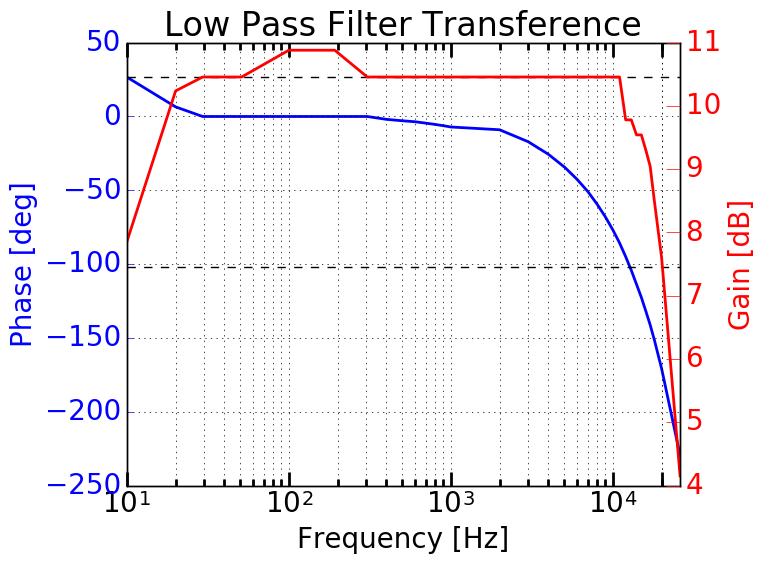
\includegraphics[width=12cm]{transference}
 \caption{Transferencia del circuito pasa bajos. En rojo la ganancia y en azul el desfase.}
 \label{fig:lowPassFilterTransference}
\end{figure}


\subsection{Potencia transmitida}

Para la medición de la potencia transmitida del radar se utilizó el analizador de espectros conectado en el cable que une la antena transmisora con el resto de la electrónica del radar. La figura \ref{fig:txPowerConnections} muestra el banco de trabajo utilizado para realizar la medición.

\begin{figure}[H]
 \centering
 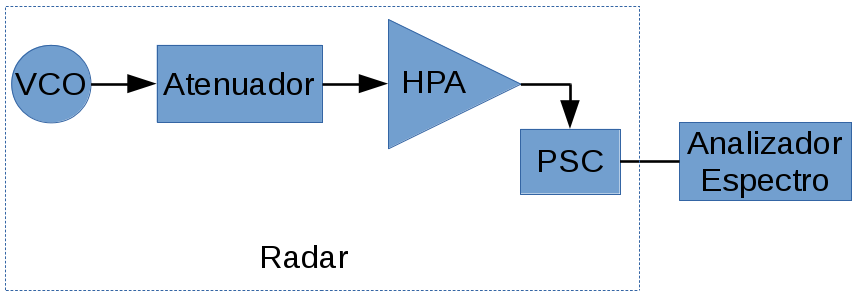
\includegraphics[width=10cm]{txPowerWorkbench}
 \caption{Banco de medición, potencia transmitida del radar.}
 \label{fig:txPowerConnections}
\end{figure}

La tabla \ref{tab:PNAConfigTxPower} resume las configuraciones utilizadas en el analizador de espectros para la medición y la figura \ref{fig:txPowerMeasurements} muestra el resultado de la medición.

\begin{table}[H]
  \caption{Configuración del analizador de espectros para medir la potencia transmitida del radar.}
  \centering
  \label{tab:PNAConfigTxPower}
  \begin{tabular}{l c c}
  \toprule
  \textbf{Característica} & \textbf{Configuración} & \textbf{Unidad} \tabularnewline
  \midrule
  Mode & ANALYZER & \tabularnewline

  Center Freq & 2434262820,514000 & \si{\hertz} \tabularnewline

  Freq Offset & 0,000000 & \si{\hertz} \tabularnewline

  Span & 1000000000,000000 & \si{\hertz} \tabularnewline

  x-Axis & LIN & \tabularnewline

  Start & 1934262820,514000 & \si{\hertz} \tabularnewline

  Stop & 2934262820,514000 & \si{\hertz} \tabularnewline

  Ref Level & 18,000000 & \si{\dBm} \tabularnewline

  Level Offset & 0,000000 & \si{\deci\bel} \tabularnewline

  Ref Position & 100,000000 & \si{\percent} \tabularnewline

  y-Axis & LOG & \tabularnewline

  Level Range & 50,000000 & \si{\deci\bel} \tabularnewline

  Rf Att & 70,000000 & \si{\deci\bel} \tabularnewline

  RBW & 10000000,000000 & \si{\hertz} \tabularnewline

  VBW & 10000000,000000 & \si{\hertz} \tabularnewline

  SWT & 0,002500 & \si{\second} \tabularnewline

  Trace Mode & CLR/WRITE & \tabularnewline

  Detector & RMS & \tabularnewline

  Sweep Count & 0 & \tabularnewline

  \bottomrule
  \end{tabular}
\end{table}

En la figura \ref{fig:txPowerMeasurements} se puede observar que la potencia transmitida por el radar es de $\SI{11.87}{\dBm}$ en una frecuencia central igual a $\SI{2.43}{\giga\hertz}$ y que el piso de ruido para esta medición se encuentra entre los $\SI{-14}{\dBm}$ y $\SI{-17.4}{\dBm}$. De esta forma se valida el requerimiento \ref{req:l2_txPower}.

\begin{figure}[H]
 \centering
 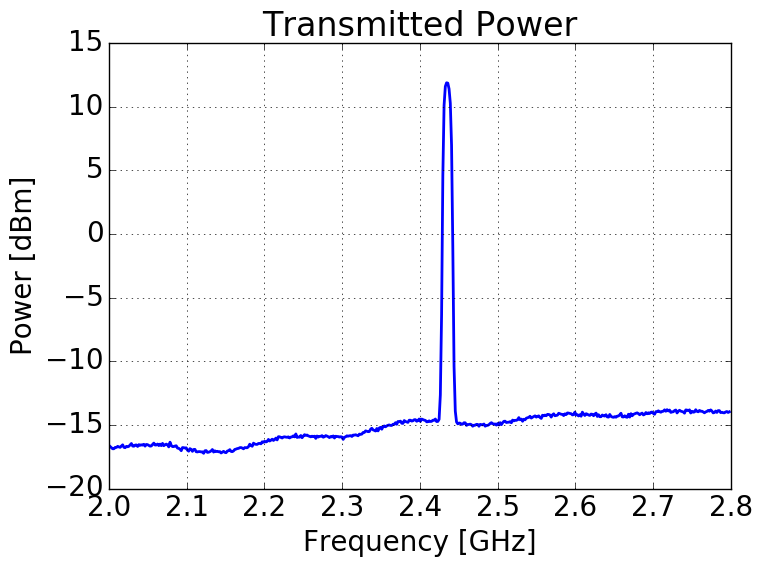
\includegraphics[width=9cm]{txPower}
 \caption{Potencia transmitida del radar medida con un PNA.}
 \label{fig:txPowerMeasurements}
\end{figure}


\subsection{Ancho de banda}

Para la medición del ancho de banda transmitido se utiliza el analizador de espectros conectado en el cable que une la antena transmisora con el resto de la electrónica del radar. La figura \ref{fig:bartPowerConnections} muestra el banco de trabajo utilizado para realizar la medición.

\begin{figure}[H]
 \centering
 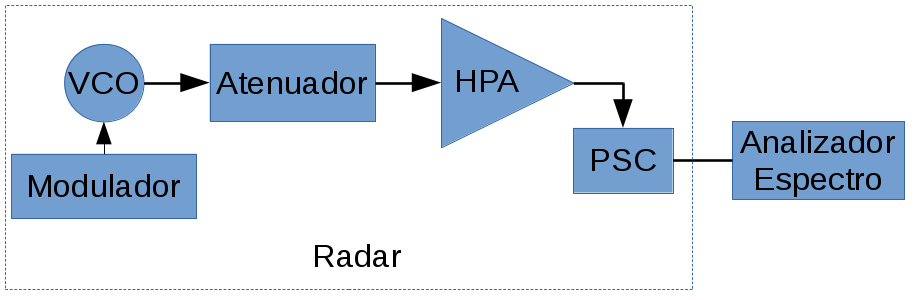
\includegraphics[width=10cm]{bartPowerWorkbench}
 \caption{Banco de medición, cabeza de chirp transmitida del radar.}
 \label{fig:bartPowerConnections}
\end{figure}

La tabla \ref{tab:PNAConfigBartPower} resume las configuraciones utilizadas en el analizador de espectros para la medición y la figura \ref{fig:bartPowerMeasurements} muestra el resultado de la medición.

\begin{table}[H]
  \caption{Configuración del analizador de espectros, medición del BW transmitido del radar.}
  \centering
  \label{tab:PNAConfigBartPower}
  \begin{tabular}{l c c}
  \toprule
  \textbf{Característica} & \textbf{Configuración} & \textbf{Unidad} \tabularnewline
  \midrule
  Mode & ANALYZER & \tabularnewline

  Center Freq & 2450288461,540000 & \si{\hertz} \tabularnewline

  Freq Offset & 0,000000 & \si{\hertz} \tabularnewline

  Span & 1000000000,000000 & \si{\hertz} \tabularnewline

  x-Axis & LIN & \tabularnewline

  Start & 1950288461,540000 & \si{\hertz} \tabularnewline

  Stop & 2950288461,540000 & \si{\hertz} \tabularnewline

  Ref Level & 18,000000 & \si{\dBm} \tabularnewline

  Level Offset & 0,000000 & \si{\deci\bel} \tabularnewline

  Ref Position & 100,000000 & \si{\percent} \tabularnewline

  y-Axis & LOG & \tabularnewline

  Level Range & 50,000000 & \si{\deci\bel} \tabularnewline

  Rf Att & 70,000000 & \si{\deci\bel} \tabularnewline

  RBW & 10000000,000000 & \si{\hertz} \tabularnewline

  VBW & 10000000,000000 & \si{\hertz} \tabularnewline

  SWT & 0,002500 & \si{\second} \tabularnewline

  Trace Mode & MAXHOLD & \tabularnewline

  Detector & RMS & \tabularnewline

  Sweep Count & 0 & \tabularnewline
  \bottomrule
  \end{tabular}
\end{table}

\begin{figure}[H]
 \centering
 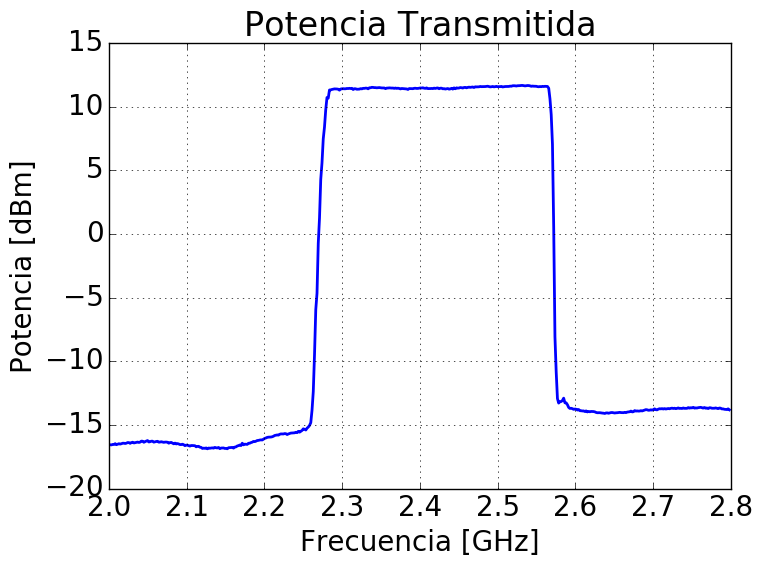
\includegraphics[width=10cm]{chripHeadPower}
 \caption{Potencia transmitida del radar medida con un analizador de espectros.}
 \label{fig:bartPowerMeasurements}
\end{figure}

Se puede observar que el ancho de banda de la señal transmitida, a $\SI{-3}{\dB}$ con respecto al pico, es igual a $\SI{291.67}{\mega\hertz}$. A su vez, la potencia de la señal es de $\SI{12}{\dBm}$ mientras que el piso de ruido es de $\SI{-15}{\dBm} \pm \SI{2}{\dBm}$. De esta forma se verifica el requerimiento \ref{req:l2_bw}.


\subsection{Parámetros S de las antenas} \label{ssc:sParameters}

Esta medición está diseñada para caracterizar el comportamiento de las antenas tanto de forma individual, midiendo el coeficiente de reflexión $S_{11}$ de cada una, como de forma grupal, midiendo el coeficiente de transmisión $S_{21}$ entre las mismas. Idealmente estos valores deberían ser 0, dado que mientras más alejado a dicho valor sea el $S_{11}$, menor es la potencia que ingresa a la antena. En cambio, el parámetro $S_{21}$ está relacionado directamente con el acoplamiento mutuo entre las antenas. Mientras mayor es dicho valor, mayor potencia recibe la antena receptora, lo cual es un efecto indeseado dado que ya se estaría recibiendo señal sin siquiera haber presencia de un blanco iluminado a caracterizar.

El banco de medición está compuesto por un VNA en donde cada canal del mismo está conectado a una antena del radar, de esta forma  la señal se transmite por una antena y se recibe a través de la segunda, ver figura \ref{fig:sParamsConnections}.
\begin{figure}[H]
 \centering
 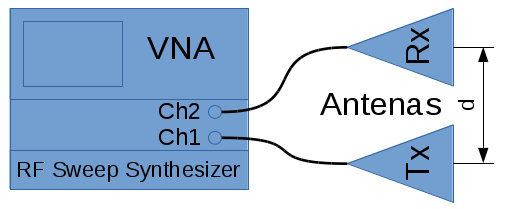
\includegraphics[width=8cm]{sParamsAntenaWorkbench}
 \caption{Banco de medición, parámetros S de las antenas.}
 \label{fig:sParamsConnections}
\end{figure}

Como las antenas son plarimétricas, se repitió la medición en todas las posibles combinaciones de polarizaciones, HH, HV, VH y VV. Es importante notar que la distancia entre los centros de las antenas permaneció invariante e igual a $\SI{15.5}{\centi\meter}$. La figura \ref{fig:sParametersMeasurements} posee los resultados de los cuatro ensayos.

\begin{figure}[H]
  \centering
  \begin{subfigure}{0.47\textwidth}
    \centering
    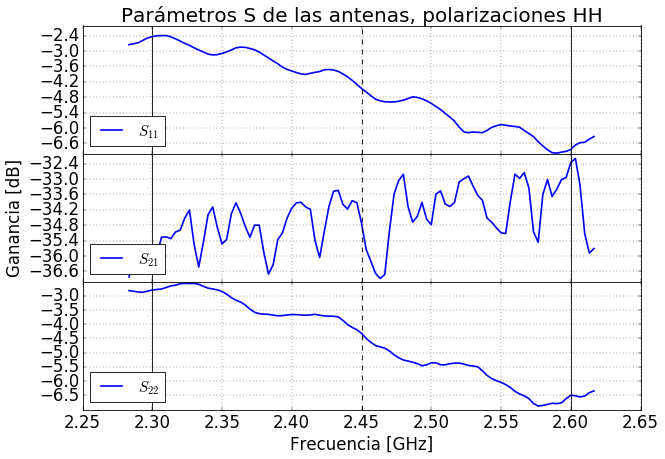
\includegraphics[width=7cm]{SParamsHH}
    \caption{Polarización HH}
    \label{subfig:hhPol}
  \end{subfigure}
  \begin{subfigure}{0.47\textwidth}
    \centering
    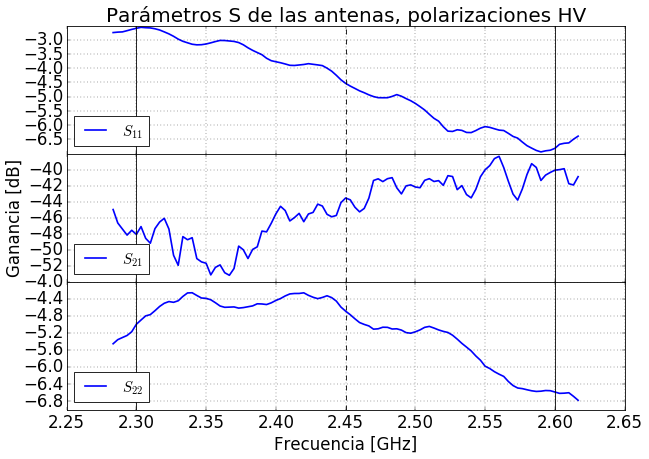
\includegraphics[width=7cm]{SParamsHV}
    \caption{Polarización HV}
    \label{subfig:hvPol}
  \end{subfigure}

  \begin{subfigure}{0.47\textwidth}
    \centering
    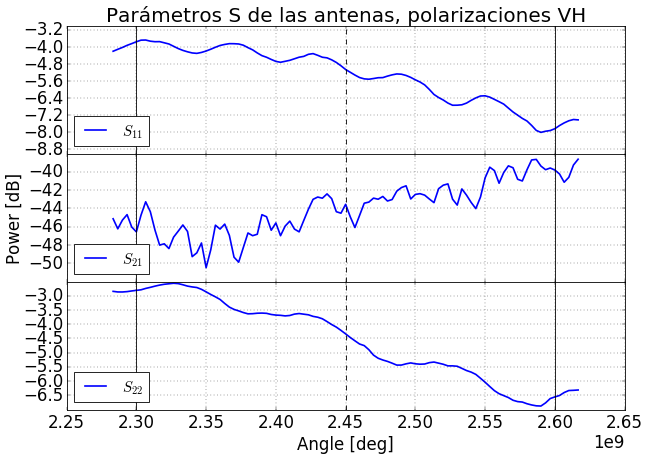
\includegraphics[width=7cm]{SParamsVH}
    \caption{Polarización VH}
    \label{subfig:vhPol}
  \end{subfigure}
  \begin{subfigure}{0.47\textwidth}
    \centering
    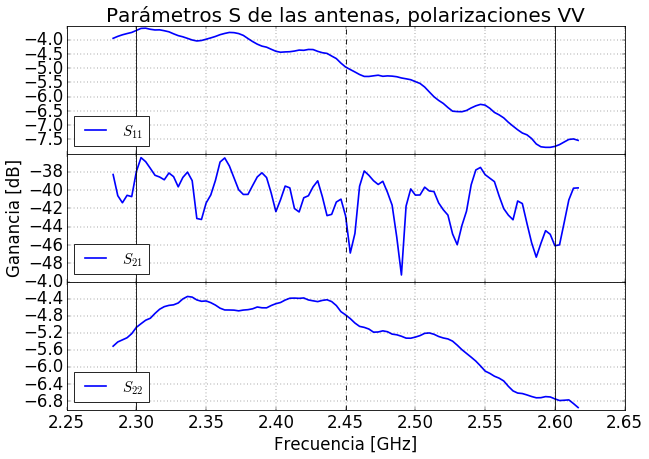
\includegraphics[width=7cm]{SParamsVV}
    \caption{Polarización VV}
    \label{subfig:vvPol}
  \end{subfigure}
  \caption{Mediciones de parámetros S de las antenas en todas las combinaciones de polarizaciones. \ref{subfig:hhPol} HH, \ref{subfig:hvPol} HV, \ref{subfig:vhPol} VH y \ref{subfig:vvPol} VV.}
  \label{fig:sParametersMeasurements}
\end{figure}

Se puede apreciar que si bien los coeficientes de reflexión son similares entre polarizaciones, todos muestran una gran variación de respuesta a lo largo de la frecuencia de trabajo, llegando a ser de hasta $\SI{4.6}{\dB}$. Por el lado de la variación del coeficiente de transmisión, la polarización HH solamente está en el orden de los $\SI{4.5}{\dB}$. En cambio para el resto de las polarizaciones, la misma resulta ser del orden de los $\SI{12}{\dB}$.

La tabla \ref{tab:antennasParameters} resume los valores medidos de cada parámetros S a la frecuencia central. Se puede apreciar que los coeficientes de reflexión de cada antena en cada polarización permanece invariante ante las combinaciones de polarizaciones utilizadas. A su vez, se puede apreciar que el coeficiente de transmisión directo permanece casi igual al coeficiente de transmisión inverso y que dichos coeficientes también son iguales entre las polarizaciones HV y VH. Por último, cabe destacar que las polarizaciones HH poseen un mayor coeficiente de transmisión que las VV en un orden de $\SI{8}{\dB}$.

\begin{table}[htb]
  \caption{Parámetros S de las antenas medidos con un VNA a frecuencia central.}
  \centering
  \label{tab:antennasParameters}
  \begin{tabular}{l *{4}{S[table-auto-round, table-format=-2.2]}}
  \toprule
  \multirow{2}{*}{\textbf{Parámetro S}} & \multicolumn{4}{c}{\textbf{Polarizaciones}} \tabularnewline
  \cmidrule{2-5}
  & HH & HV & VH & VV \tabularnewline
  \midrule
  
  $S_{11}$ & -4.46033873376335 & -4.53492363950625 & -5.06302223793916 & -4.95964466600015 \tabularnewline

  $S_{12}$ & -34.8204780020621 & -43.4389116307712 & -43.5577358595805 & -42.7387139376128 \tabularnewline

  $S_{21}$ & -34.7141043352772 & -43.5629806134325 & -43.4259094492972 & -42.8482094658858 \tabularnewline

  $S_{22}$ & -4.32197124367156 & -4.69545953806287 & -4.34205880309025 & -4.78356133012197 \tabularnewline

  \bottomrule
  \end{tabular}
\end{table}


\subsection{Diagrama de Radiación}

Para esta medición se desconectó del radar la antena receptora y se la conectó en el analizador de espectros a una distancia igual a $\SI{1.427}{\meter}$ para medir la potencia recibida por el radar, ver figura \ref{fig:radiationPatternConnections}. A la antena transmisora se la fue rotando a medida que se tomaban muestras para obtener el diagrama de radiación. Por último, tanto a la antena transmisora como la receptora se le fueron cambiando las polarizaciones para obtener el diagrama en todas las posibles combinaciones, HH, HV, VH y VV.
\begin{figure}[htb]
 \centering
 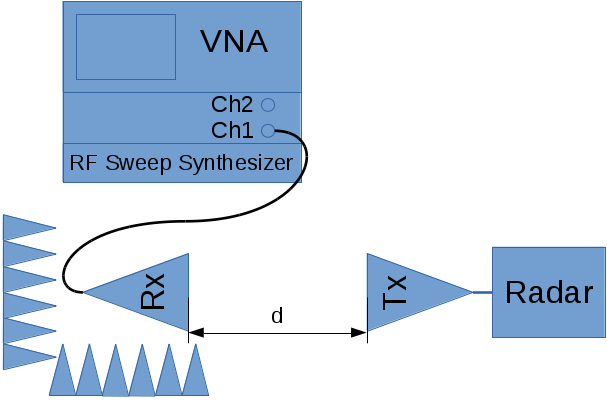
\includegraphics[width=8cm]{RadiatingPatternAntenaWorkbench}
 \caption{Banco de medición, diagrama de radiación entre antenas.}
 \label{fig:radiationPatternConnections}
\end{figure}

Es importante notar en la imagen \ref{fig:radiationPatternConnections} que la antena receptora se la colocó frente a absorbedores para disminuir la potencia recibida proveniente de ecos en las paredes de la sala en que se realizó la medición. La tabla \ref{tab:PNAConfigRadiationPattern} resume las configuraciones utilizadas en el analizador de espectros para las mediciones.

\begin{table}[H]
  \caption{Configuración del analizador de espectros, medición del diagrama de radiación.}
  \centering
  \label{tab:PNAConfigRadiationPattern}
  \begin{tabular}{l c c}
  \toprule
  \textbf{Característica} & \textbf{Configuración} & \textbf{Unidad} \tabularnewline
  \midrule
  Mode & ANALYZER & \tabularnewline

  Center Freq & 2434262820,514000 & \si{\hertz} \tabularnewline

  Freq Offset & 0,000000 & \si{\hertz} \tabularnewline

  Span & 100000000,000000 & \si{\hertz} \tabularnewline

  x-Axis & LIN & \tabularnewline

  Start & 2384262820,514000 & \si{\hertz} \tabularnewline

  Stop & 2484262820,514000 & \si{\hertz} \tabularnewline

  Ref Level & -9,000000 & \si{\dBm} \tabularnewline

  Level Offset & 0,000000 & \si{\dB} \tabularnewline

  Ref Position & 100,000000 & \si{\percent} \tabularnewline

  y-Axis & LOG & \tabularnewline

  Level Range & 100,000000 & \si{\dB} \tabularnewline

  Rf Att & 5,000000 & \si{\dB} \tabularnewline

  RBW & 2000000,000000 & \si{\hertz} \tabularnewline

  VBW & 50,000000 & \si{\hertz} \tabularnewline

  SWT & 2,500000 & \si{\second} \tabularnewline

  Trace Mode & CLR/WRITE & \tabularnewline

  Detector & RMS & \tabularnewline

  Sweep Count & 0 & \tabularnewline
  \bottomrule
  \end{tabular}
\end{table}

La tabla \ref{tab:antennaPattern} resume los resultados de las mediciones realizadas y la imagen \ref{fig:patterns} muestra los diagramas de radiación. Se puede observar que el ancho del lóbulo principal para las polarizaciones HH y VV son muy similares, aproximadamente de unos $\SI{50}{\degree}$ y que las ganancias máximas del mismo rondan los $\SI{-22}{\dB}$. En cambio, se nota que para HH los lóbulos secundarios son $\SI{3}{\dB}$ mayores y los mismos se encuentran a $\SI{3.8}{\dBc}$ para HH y $\SI{6.55}{\dBc}$ para VV.

Por último, comparando los gráficos co-polares con respecto al cross-polar, se puede observar que el rechazo por polarización cruzada es de $\SI{18}{\dB}$, dado que la ganancia recibida es de $\SI{-40}{\dB}$ frente a los $\SI{-22}{\dB}$ de las co-polares, para el centro del lóbulo principal. A su vez se observa que los lóbulos secundarios poseen una ganancia mayor, llegando a los $\SI{-37}{\dB}$.

\begin{figure}
  \centering
  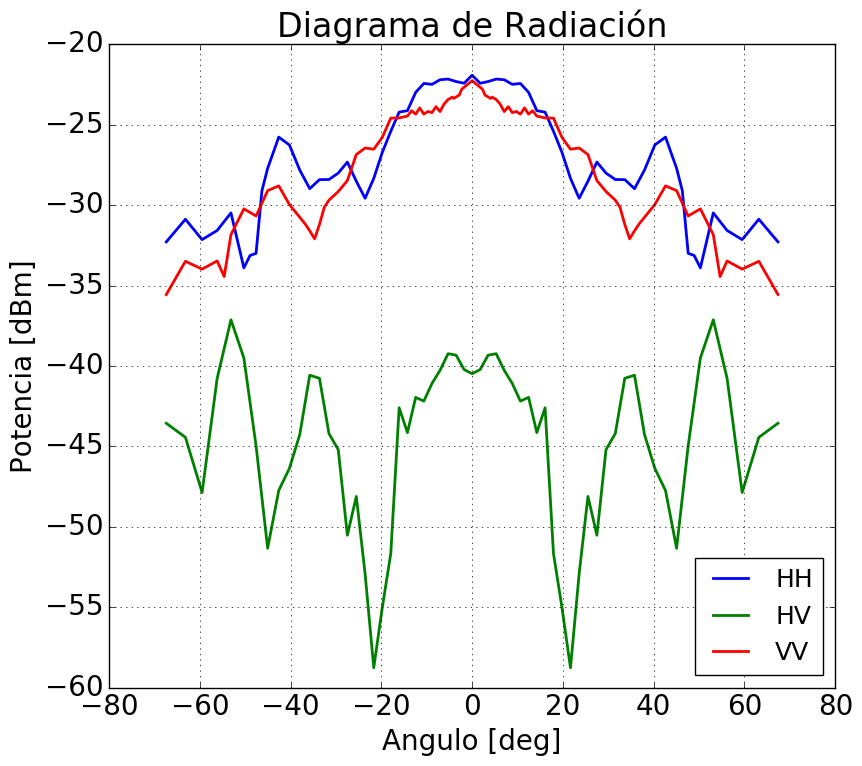
\includegraphics[width=10cm]{patterns}
  \caption{Diagrama de radiación del radar en distintas combinaciones de polarizaciones, HH, HV y VV.}
  \label{fig:patterns}
\end{figure}

\begin{table}[H]
  \caption{Mediciones diagrama de radiación entre polarizaciones.}
  \centering
  \label{tab:antennaPattern}
  \begin{tabular}{*{5}{S[table-auto-round, table-format=-2.2]}}
  \toprule
  \multirow{2}{*}{\textbf{ángulos entre antenas [$\si{\degree}$]}} & \multicolumn{4}{c}{\textbf{Potencia transmitida en polarizaciones}} \tabularnewline
  \cmidrule{2-5}
   & HH & HV & VH & VV \tabularnewline
  \midrule
  0.0 & -21.914052963256836 & -40.480464935302734 & -40.480464935302734 & -22.251615524291992 \tabularnewline

  1.91021317171 & -22.4134578704834 & -40.224273681640625 & -40.224273681640625 & -22.784189224243164 \tabularnewline

  3.82255372927 & -22.30802345275879 & -39.3284797668457 & -39.3284797668457 & -23.145263671875 \tabularnewline

  5.73917047727 & -22.154735565185547 & -39.235477447509766 & -39.235477447509766 & -23.423660278320312 \tabularnewline

  7.66225566077 & -22.194988250732422 & -40.26947021484375 & -40.26947021484375 & -24.174240112304688 \tabularnewline

  9.59406822686 & -22.48287582397461 & -41.09086608886719 & -41.09086608886719 & -24.239660263061523 \tabularnewline

  11.5369590328 & -22.42629051208496 & -42.18770980834961 & -42.18770980834961 & -24.336830139160156 \tabularnewline

  13.4933988216 & -22.981735229492188 & -41.95241928100586 & -41.95241928100586 & -24.332292556762695 \tabularnewline

  15.4660099534 & -24.11693000793457 & -44.143924713134766 & -44.143924713134766 & -24.45547866821289 \tabularnewline

  17.4576031237 & -24.21193504333496 & -42.601112365722656 & -42.601112365722656 & -24.572660446166992 \tabularnewline

  19.4712206345 & -25.39852523803711 & -51.66230010986328 & -51.66230010986328 & -24.58316993713379 \tabularnewline

  21.5101882669 & -26.707298278808594 & -55.01024627685547 & -55.01024627685547 & -25.775318145751953 \tabularnewline

  23.5781784782 & -28.32943344116211 & -58.773075103759766 & -58.773075103759766 & -26.516315460205078 \tabularnewline

  25.6792886195 & -29.568967819213867 & -52.928672790527344 & -52.928672790527344 & -26.44162368774414 \tabularnewline

  27.8181392847 & -28.507495880126953 & -48.11441421508789 & -48.11441421508789 & -26.84745216369629 \tabularnewline

  30.0 & -27.317434310913086 & -50.52842330932617 & -50.52842330932617 & -28.46544075012207 \tabularnewline

  32.2309526355 & -28.002696990966797 & -45.20555877685547 & -45.20555877685547 & -29.152206420898438 \tabularnewline

  34.5181078411 & -28.401615142822266 & -44.20515060424805 & -44.20515060424805 & -29.684959411621094 \tabularnewline

  36.8698976458 & -28.40848731994629 & -40.76640701293945 & -40.76640701293945 & -31.19536590576172 \tabularnewline

  39.2964802392 & -28.97147560119629 & -40.5757942199707 & -40.5757942199707 & -31.591350555419922 \tabularnewline

  41.8103148958 & -27.810001373291016 & -44.27327346801758 & -44.27327346801758 & -30.774405479 \tabularnewline

  44.4270040008 & -26.254615783691406 & -46.36780548095703 & -46.36780548095703 & -29.957460403442383 \tabularnewline

  47.1665719339 & -25.764413833618164 & -47.74458694458008 & -47.74458694458008 & -28.79700469970703 \tabularnewline

  50.0554948102 & -27.705350875854492 & -51.336891174316406 & -51.336891174316406 & -29.092802047729492 \tabularnewline

  53.1301023542 & -32.99269104003906 & -44.96973419189453 & -44.96973419189453 & -30.67097282409668 \tabularnewline

  56.4426902381 & -33.899192810058594 & -39.50574493408203 & -39.50574493408203 & -30.22670555114746 \tabularnewline

  60.0735651334 & -30.478853225708008 & -37.128719329833984 & -37.128719329833984 & -31.830547332763672 \tabularnewline

  64.1580672368 & -31.572757720947266 & -40.781593322753906 & -40.781593322753906 & -33.468048095703125 \tabularnewline

  68.9605302187 & -32.14019012451172 & -47.87135314941406 & -47.87135314941406 & -33.976505279541016 \tabularnewline

  75.164888418 & -30.873291015625 & -44.438751220703125 & -44.438751220703125 & -33.48764419555664 \tabularnewline

  90.0 & -32.28058624267578 & -43.56352233886719 & -43.56352233886719 & -35.55542755126953 \tabularnewline
  \bottomrule
  \end{tabular}
\end{table}


\section{Resumen}

En este capítulo se detallaron todos los subsistemas de hardware que componen al radar. Los mismos son el modulador, la cadena de RF, las antenas transmisoras y receptoras, el filtro pasa bajos y por último el gabinete. A su vez se midió cada uno de los mismos para verificar su correcto funcionamiento y cumplimiento de los requerimientos de nivel 2.

El circuito modulador fue construido de tal forma de poder transmitir más de un tipo de modulación ante la posibilidad de realizar futuros ensayos con distintos tipos de señales transmitidas, requerimiento \ref{req:l2_mod}. Las posibles modulaciones son diente de sierra creciente o decreciente, triangular y sinusoidal.

La potencia transmitida por la cadena de RF sin modular es igual a $\SI{1.87}{\dBm}$, al modular con el diente de sierra se obtiene un ancho de banda igual a $\SI{291.67}{\MHz}$.

Tanto para aumentar la directividad de las antenas como para que cada una sea polarimétrica, se hace uso de cavidades, que por simplicidad son cilíndricas. En un paso futuro, para asegurar la polarimetría se deben utilizar prismas rectangulares y para disminuir el cross-talk entre polarizaciones de una misma antena, se debe separar cada monopolo en una longitud de onda. Con respecto a las mediciones de comportamiento de las antenas, se puede observar que el coeficiente de reflexión ronda los $\SI{-5}{\dB}$ y que los coeficientes de transmisión entre polarizaciones ronda los $\SI{-43}{\dB}$ salvo para HH que ronda los $\SI{-35}{\dB}$.

Por último, se midió el diagrama de radiación a una distancia de $\SI{1.427}{\meter}$, se puede determinar que el rechazo de polarización cruzada es de $\SI{18}{\dB}$ siendo la ganancia recibida del centro del lóbulo principal para el caso co-polar igual a $\SI{-22}{\dB}$. Por último, los lóbulos secundarios se encuentran a $\SI{50}{\degree}$ y los mismos poseen una potencia de $\SI{3.8}{\dBc}$ para el caso HH y de $\SI{6.55}{\dBc}$ para el caso VV.

\chapter{Resultados previstos} \label{ch:results}

A partir de las actividades propuestas en el plan se prevé:

\begin{enumerate}
    \item Obtener un simulador del funcionamiento del radar completo en donde se puedan modificar propiedades tanto de transmisión y recepción del radar como de distancia y propiedades del cuerpo iluminado.

    \item Armar el prototipo de ingeniería del radar FMCW.

    \item Validar y caracterizar los distintos subsistemas del radar construido.

    \item Identificar las principales fuentes de incertidumbres para la determinación experimental de la matriz de dispersión de un blanco con el radar construido.

    \item Establecer criterios de mejoras para disminuir y mantener controladas dichas fuentes de incertidumbres.
\end{enumerate}



% ********************************** Bibliography ******************************
% \begin{spacing}{0.9}

% To use the conventional natbib style referencing
% Bibliography style previews: http://nodonn.tipido.net/bibstyle.php
% Reference styles: http://sites.stat.psu.edu/~surajit/present/bib.htm

% \bibliographystyle{apalike}
\bibliographystyle{unsrt} % Use for unsorted references  
%\bibliographystyle{plainnat} % use this to have URLs listed in References
\cleardoublepage
\bibliography{References/Miniradar} % Path to your References.bib file

% \end{spacing}

\begin{comment}
	\section{INTRODUCCIÓN}
    
Las antenas de arreglo de fase controlada [\ref{sarAntenna}] son utilizadas en 
aplicaciones de todo tipo, por ejemplo comunicaciones de móviles 
[\ref{ppr:mutual-ext1}], aéreas [\ref{ppr:punc-ext1}] y espaciales 
[\ref{ppr:dist1}][\ref{ppr:classic8}]. 

Para generar diversos productos, por ejemplo imágenes satelitales en radares de
apertura sintética [\ref{ppr:puncTrgt1}], 
es necesario que estén correctamente calibradas [\ref{ppr:classic1}] 
[\ref{ppr:classic2}][\ref{ppr:classic3}]. Esto implica, que las tolerancias de
fases y amplitudes se mantengan en el tiempo y/o sus valores sean bien conocidas
para cada elemento del arreglo.

Generalmente, este tipo de antenas son calibradas en tierra utilizando fuentes 
externas de campo lejano o cercano [\ref{ppr:mutual1}]. Sin embargo, en 
aplicaciones aéreas o espaciales, la utilización de dichas fuentes es impráctica
o difícil de implementar [\ref{ppr:mutual3}]. Resulta fundamental un esquema de
calibración interna que permita tener bajo control estas variables. Generalmente
se implementan lazos de calibración internos [\ref{ppr:classic1}]
[\ref{ppr:classic2}][\ref{ppr:classic3}][\ref{ppr:abs-rad-ical1}]
[\ref{ppr:classic4}][\ref{ppr:classic5}][\ref{ppr:classic6}]
[\ref{ppr:classic-ext1}][\ref{ppr:classic7}][\ref{ppr:classic8}]. 
Luego se opta por caracterizar todos aquellos componentes que no entran dentro 
de dicho lazo de calibración [\ref{ppr:abs-rad-ical1}].
Este método presenta algunos inconvenientes. Por dar un par de ejmplos se puede
mencionar que los recursos necesarios (tiempo, personal) durante la campaña de 
ensayos previa al lanzamiento impactan en todo el desarrollo de actividades, o
que las consecuencias que puede traer el hecho de que la caracterización no sea
válida porque un determinado componente envejece con el paso del tiempo.

En este contexto, se investiga y propone un método que permita reducir costos 
asociados a la calibración y por ende a los proyectos:

\begin{enumerate}
    \item Evitando la necesidad de realizar caracterizaciones previas de la 
antena de arreglo de fase.
    \item Permitiendo conocer en tiempo real, y para el estado real de la antena
, los valores reales de fase y amplitud en vuelo que transmite la antena, 
independientemente de su estado de envejecimiento.
\end{enumerate}

En este sentido se investiga y aprovecha el concepto acoplamiento mutuo 
inherente entre los módulos radiantes de la antena [\ref{ppr:mutual3}], pero de
manera complementaria al enfoque tradicional. 

En esta tesis se realizarán las siguientes tareas:

\begin{enumerate}
    \item Se explicarán las ventajas y desventajas del método propuesto respecto
del tradicional.
    \item Se analizarán y propondorán los requerimientos para poder 
implementarlo.
    \item Se desarrollará un modelo de antena de arreglo de fase polarimétrico 
básico representativo en parámetros S \ref{pr:parameters}.
    \item Se añadirán al mismo parámetros de dispersión de comportamiento que 
permitan analizar su comportamiento.
    \item Se realizará un modelo de calibración que será implementado 
algoritimicamente.
\end{enumerate}

\subsection{DEFINICIÓN}

{\textbf{Antena de arreglo de fase}} (en inglés: phased array) es un conjunto de
antenas en que las fases relativas de las señales con que se alimenta cada 
antena se varían intencionadamente con objeto de alterar el diagrama de 
radiación del conjunto. Lo normal es reforzar la radiación en una dirección 
concreta y suprimirla en direcciones indeseadas. Si todos los elementos del 
arrreglo de fase están contenidos en el mismo plano y la señal con que se 
alimentan es de la misma fase, entonces se estará reforzando la dirección 
perpendicular a ese plano. Si se altera la fase relativa de las señales se podrá
 \enquote*{mover} el haz (en realidad lo que se está haciendo es cambiar la 
dirección en la cual las interferencias son constructivas). Se consigue de este
modo hacer barridos sin necesidad de movimiento físico, con la ventaja añadida
de que se pueden barrer ángulos del orden de miles de grados por segundo. Esto
permite utilizar la antena para compaginar simultáneamente funciones de 
detección y de seguimiento muchos blancos individuales, asi como para obtener 
imágenes de apertura sintética. Su uso se va extendiendo debido a la 
confiabilidad derivada del hecho de que no tienen partes móviles. Casi todos los
radares militares modernos se basan en phased arrays, relegando los sistemas 
basados en antenas rotatorias a aplicaciones donde el costo es un factor 
determinante (tráfico aéreo, meteorología, etc) Su uso está también extendido en
aeronaves militares debido a su capacidad de seguir múltiples objetivos. El 
primer avión en usar uno fue el B-1B Lancer, y el primer caza, el MiG-31 ruso.\\

{\textbf{Calibración interna}} es colocar sensores que permitan la medición 
directa u indirecta de los distintos parámetros del sistema en vuelo. 

Estas mediciones obtenidas con este sistema son útiles solamente al utilizarlas
en conjuto a los resultados de los test realizados en tierra, los cuales definen
la relación entre lo observado y la performance de los párametros del sistema. 
Ejemplos de satélites para los cuales se utilizó calibración interna son el 
E-ERS-1 y el SIR-C.
    
Los tests realizados en tierra para dichos sistemas complejos son sobre la
electrónica de RF, la electrónica digital y la antena sobre temperatura; para 
los cuales es preferible realizarlos, cuando sea posible, en un ambiente al 
vacío. Los parámetros clave del sistema, como: potencia transmitida, pérdidas de
transmisión o recepción, ganancia de recepción, ganancia y patrón de la antena, 
linealidad de la electrónica digital/RF, rango dinámico, y fase/amplitud vs 
estabilidad de la frecuencia son medidos en función de la temperatura para cada 
seteo de ganancia del radar y PRF (Pulse Repetition Frequency). Los elementos de
calibración, como medidores de temperatura, de corriente y de potencia, podrán 
permitir la determinación de la performance del sistema en función de la 
variación de dichos parámetros.
    
Esta técnica asume que la variación en la performance del sistema puede ser 
modelada en función de los parámetros observables. También, se asume que los 
componentes de calibración están correctamente calibrados y son estables en el 
paso del tiempo. Además de estos tests, en la mayoría de los sistemas de radar 
se realizan mediciones de componentes de RF utilizando loops de calibración.
		
\section{MOTIVACIÓN}

A la hora de adquirir imágenes satelitales es crucial que se conozca 
perfectamente la señal emitida y recibida por la antena. Ya sea por 
envejecimiento de los componentes [\ref{ppr:mutual1}] o por variaciones de 
temperaturas se observan dispersiones de las mismas [\ref{ppr:sim1}]. 


El método de calibración tradicional, por lazos de calibración internos, permite
calibrar una antena de arreglo de fase, aunque adolece de algunos defectos entre
los cuales se incluyen:

\begin{enumerate}
    \item Una degradación o directamente rotura de un elemento radiante, el cual
está fuera del lazo de calibración interno, no es detectado por la calibración 
interna.
    \item Existen elementos que quedan fuera del lazo de calibración interno. 
Como por ejemplo los circuladores. Esto lleva a la necesidad de realizar 
caracterizaciones en tierra lo cual implica consumo de recursos de proyecto 
importantes, además de tener que confiar que dicha caracterización será válida 
(o sea que no habrá envejecimiento de los mismo) luego durante vuelo en toda la
vida útil de la antena.
    \item Cada lazo de calibración no se interrelaciona con el resto haciendo 
que no se pueda disminuir el error de medición por multiplicidad de caminos.
\end{enumerate}

Esto lleva a investigar opciones superadoras, que den lugar a un método de 
calibración que permita complementar al tradicional evitando la necesidad de 
realizar costosas caracterizaciones en tierra, previendo que los componentes en
vuelo puedan envejecer y por ende dichas caracterizaciones no ser más validas, 
permitiendo detectar fallas en elementos que en la calibración interna 
tradicional quedan fuera del lazo de calibración, y disminuyendo la 
incertidumbre en la determinación de la fase y amplitud de salida.

El método que se propone en esta tesis, denominado de \enquote*{método de 
calibración interna complementada por acoplamientos mutos (MCINCAM)} toma la 
idea de mediciones por acoplamiento mutuo [\ref{ppr:mutual1}][\ref{ppr:mutual2}]
[\ref{ppr:mutual3}][\ref{ppr:mutual-ext1}], para integrarla de manera 
complementaria al método tradicional, sin necesidad de agregar hardware 
adicional, y además establece los requerimientos electrónicos para poder 
implementarla. En esta tesis además se realiza un modelo ad hoc, en parámetros 
S, de antena, para mostrar la eficacia del método. 


\section{Objetivo de la tesis}

La presente tesis tiene varios objetivos:

\begin{enumerate}
    \item Presentar conceptualmente el método tradicional de calibración interna
de una antena polarimétrica que abarque el sistema completo de transmisión/
recepción. con sus virtudes y defectos. Mencionar algunas misiones de ejemplo en
las cuales el mismo se ha utilizado.
    \item Investigar, desarrollar y presentar conceptualmente un método 
alternativo de calibración interna que introduzca mejoras al método tradicional 
sin necesidad de introducir hardware adicional y con la premisa fundamental de 
reducir los costos asociados a las caracterizaciones que el método tradicional 
incluye. Introducir los requerimientos necesarios para poder implementarlo.
    \item Investigar, desarrollar y presentar (generar) los algoritmos que 
permitan representar el modelo de antena polarimétrico (modelo de capa física) 
que serán utilizados para poder comparar el método tradicional y el alternativo.
Dichos modelos deben representar el comportamiento en RF básico de las señales 
al propagarse por el sistema.
    \item Generar los algoritmos que permitan correr el algoritmo de calibración
alternativo de manera de poder comparar ambos métodos.
    \item Sacar conclusiones respecto a los pros y contras del método propuesto,
en particular en referencia al método tradicional, por medio de algunos 
parámetros objetivos como ser tiempo de calibración, caracterizaciones 
necesarias, incertidumbre de medición, entre otros.
\end{enumerate}    


\section{Especificaciones del problema}

\begin{itemize}
    \item La aplicación debera reproducir el comportamiento en RF de los 
elementos individuales: cables, psc, TRM, elementos radiantes.

    \item La aplicación deberá reproducir el comportamiento del sistema el cual 
será LTI (lineal e invariante en el tiempo).
    
    \item La antena debe estar compuesta por defasadores, atenuadores, cables, 
divisores de potencia y módulos radiantes.
    
    \item Se deben poder utilizar distintos divisores/combinadores de potencia. 
La diferencia entre ellos es la cantidad de puertos de salida.
    
    \item Los componentes de la antena deben caracterizarse utilizando 
parámetros de alta frecuencia.
    
    \item Se debe tener en cuenta el efecto que impone un componente al resto de
la antena.

    \item Se debe poder configurar la dimensión de la antena.
    \item Se debe poder configurar la distancia entre elementos radiantes.
    \item Se debe poder configurar los atributos que afecten la modelización de
cada componente de la antena. 
    
    \item Se debe poder configurar el largo de los cables.
    \item Se debe poder configurar la atenuación de los cables.
    
    \item Se debe poder configurar el error de comportamiento de cada
componente de la antena de forma independiente.

    \item Se deben poder configurar los atenuadores y defasadores a la hora de 
realizar la calibración. 

    \item La aplicación debe poder calibrar una antena polarimétrica con el 
método de calibración convencional.
    
    \item La aplicación debe poder calibrar una antena polarimétrica con el
método de calibración alternativo.
    
    \item La aplicación debe poder calibrar la potencia de transmisión y 
recepción.
    
    \item La aplicación debe poder calibrar la fase de transmisión y 
recepción.
    
    \item La aplicación debe poder calibrar en ambas polarizaciones: horizontal
y vertical.
    
    \item Se debe poder alcanzar el estado de calibración deseado partiendo 
cualquier estado inicial en los defasadores y atenuadores.
    
    \item No se puede calibrar en la misma polarización transmisión y recepción 
a la vez.
    
    \item La antena tiene que ser perfectamente plana. No deben haber 
imperfecciones.
           
    \item Se debe poder configurar la frecuencia de trabajo.

    \item Se debe poder configurar los parámetros de error (desvío estandar) 
para la ganancia y fase de la chirp utilizada entre pulsos.

    \item Se debe poder configurar los parámetros de error (desvío estandar) 
para la ganancia y fase de la chirp réplica utilizada a la hora de realizar la 
calibración convencional.
    
    \item Se debe poder configurar los parámetros de error (desvío estandar) 
para la fase de la codificación utilizada a la hora de realizar la calibración
convencional.

    \item Se debe poder simular, configurar la destrucción total de elementos de
la antena SAR como ser los TRMs.
\end{itemize}


\section{Metodología de la tesis}

		En la presente tesis se investigarán los métodos de calibraciones 
	actuales para poder determinar que ventajas, desventajas, limitaciones y 
	diferencias hay entre cada una de ellos. Se buscará tener una visión global
	de esta problemática para poder determinar y entender que posibles falencias
	puede tener este método alternativo.

		Posteriormente, se investigarán las limitaciones que poseen las antenas 
	polarimétricas para poder determinar que recaudos se deben tener en cuenta a
	la hora de desarrollar el método.

		Luego, tomando todo en cuenta, se determinarán las hipótesis necesarias
	para que el algoritmo funcione correctamente. Para la validación del método
	se realizará un modelo de antena.
		
		Finalmente, se probarán, analizarán y documentarán los resultados 
	obtenidos de la comparación entre el algoritmo propuesto y el algoritmo de
	la calibración convencional. A su vez, se dejará asentado que posibles 
	mejoras se podrían aplicar al algoritmo para determinar otros aspectos que
	están fuera del alcance de esta tesis.


\section{Estado de Situación}
		La calibración de una antena polarimétrica se ha estudiado en numerosas 
	ocasiones, abordando el problema desde distintos enfoques. A continuación se
    pueden observar los distintos métodos utilizados, clasificados por la 
    utilización o no de componentes externos.

	\[
		\substack{\text{métodos}\\de\\\text{calibración}}
		\begin{cases}
			\substack{\text{utilizan}\\\text{componentes externos}}
			\begin{cases}
				
				\text{blancos puntuales - [\ref{ppr:puncTrgt1}], 
				[\ref{ppr:puncTrgt2}], [\ref{ppr:punc-ext1}], 
				[\ref{ppr:puncTrgt3}]}\\
				\text{blancos distribuidos - [\ref{ppr:dist1}]}\\
				\text{absolute Radiometric Calibration - [\ref{ppr:absRad1}],
				[\ref{ppr:rad2}], [\ref{ppr:rad3}], [\ref{ppr:abs-rad-ical1}], 
				[\ref{ppr:rad4}], [\ref{ppr:rad5}], [\ref{ppr:rad6}], 
				[\ref{ppr:rad7}]}\\
				\text{Broadcast Reference Technique - [\ref{ppr:brdcast1}]}\\
				\text{miden deformación antena - [\ref{ppr:aligment1}], 
				[\ref{ppr:aligment2}], [\ref{ppr:aligment3}], 
				[\ref{ppr:aligment4}], [\ref{ppr:aligment5}],
				[\ref{ppr:aligment6}]}\\
				\text{utilizan calibración externa - [\ref{ppr:ext1}], 
				[\ref{ppr:ext2}], [\ref{ppr:ext3}], [\ref{ppr:punc-ext1}], 
				[\ref{ppr:classic-ext1}], [\ref{ppr:mutual-ext1}]}\\
			\end{cases}\\
			\substack{\text{no utilizan}\\\text{componentes externos}}
			\begin{cases}
				\text{calibración clásica - [\ref{ppr:classic1}], 
				[\ref{ppr:classic2}], [\ref{ppr:classic3}], 
				[\ref{ppr:abs-rad-ical1}], [\ref{ppr:classic4}], 
				[\ref{ppr:classic5}], [\ref{ppr:classic6}],
				[\ref{ppr:classic-ext1}], [\ref{ppr:classic7}],
				[\ref{ppr:classic8}]}\\
				\text{aprovechando acoplamiento mutuo - [\ref{ppr:mutual1}], 
                [\ref{ppr:mutual2}], [\ref{ppr:mutual3}], 
                [\ref{ppr:mutual-ext1}]}\\
				\text{método REV - [\ref{ppr:rev1}]}
			\end{cases}
		\end{cases}
	\]


La calibración interna es el método típicamente más utilizado pero adolece de 
algunos defectos como ser que:

\begin{itemize}
    \item Los circuladores no están incluidos dentro de dicho lazo de 
calibración interna. Esto obliga a que los mismos tengan que ser caracterizados
previamente y asegurar la estabilidad a lo largo de toda la vida útil de la
misión.
    \item Las antenas, o modulos radiantes, también quedan fuera del lazo de
calibración. Por ende, un módulo radiante que pudiese resultar dañado en vuelo,
no es detectable por el lazo interno de calibración.
    \item Durante los ensayos, se adolece de puntos de testeo que permitan 
corroborar que la potencia de salida por el modulo radiante es la esperada. No
hay acopladores direccionales entre el TRM y el modulo radiante entonces no es
posible si no es con un equipo de campo cercano poder ver la potencia de salida
de cada módulo radiante y la fase.
    \item Es necesario realizar una caracterización de la RFDN en temperatura lo
cual insume numerosos recursos y queda sujeto además a la suposición de que nada
cambien en el tiempo.
    \item Existe una incertidumbre dada reductible hasta cierto punto en la 
determinación de fase y amplitud de salida dada por lo que determina la cadena y
el camino en cuestión.
\end{itemize}

Por este motivo la calibración interna requiere de un método que complemente 
todos estos aspectos, mejorandolos. Es decir un método que:

\begin{itemize}
    \item Incorpore los circuladores al lazo de calibración interno (LCI).
    \item Incorpore los módulos radiantes al LCI.
    \item Permita durante los ensayos poder estimar la potencia real y fase con
la que emite cada uno de los módulos radiante sin la necesidad de incorporar
elementos adicionales como ser acopladoes direccionales.
    \item Evite o minimice las caracterizaciones previas que demandan una
cantidad de recursos para nada despreciable y que encarece las campañas.
    \item Permita minimizar la incertidumbre de salida en fase y ganancia.
\end{itemize}

Entre la biliografia de antenas existe un método denominado de calibración por 
acoplamiento mutuo, ver [\ref{ppr:mutual1}], [\ref{ppr:mutual2}], 
[\ref{ppr:mutual3}], [\ref{ppr:mutual-ext1}]. Este método no puede determinar la
 potencia y fase absoluta de transmisión de cada módulo radiante, solamente la 
potencia y fase relativa entre los mismos. Por ende, este método no es completo.

Se propone utilizar el método de acoplamiento mutuo como “complemento” del 
existente denominándolo método de “autocalibracion interna extendida”. Como 
ventaja, no solo se abarca todo el sistema sino que también es fácilmente 
implementable con el hardware ya existente. 

%\newgeometry{hmargin=3cm,vmargin=5cm}
%\thispagestyle{lscape}
%\begin{landscape}
 
    \section{Cronograma}
	
\begin{figure}[!htb]
 \centering
 %\includegraphics[width=1.5\textwidth]{Imagenes/CronogramaTesis.png}
 \includegraphics[width=\textwidth]{Imagenes/crono.png}
 \caption{Cronograma}
 \label{fig:crono}
\end{figure}

%    \end{landscape}
%\restoregeometry
       
    \subsection{Cronograma detallado}

En el cronograma se propone un tiempo de cuatro horas por día de trabajo, por lo tanto, las tareas quedan divididas de la siguiente forma:

\begin{itemize}
    \item 240 horas para investigar sobre los distintos métodos de calibración existentes.
    \item 80 horas para investigar sobre el funcionamiento de una antena polarimétrica.
    \item 240 horas para desarrollar un modelo de antena polarimétrica
    \item 120 horas para desarrolar la simulación del método de mutual Calibration.
    \item 60 horas para desarrollar la simulación del método de calibración interna.
    \item 100 horas para definir ensayar testear y extraer conclusiones de las 
comparaciones entre ambos métodos de calibración.
    \item 220 horas para redactar la tesis
\end{itemize}

	\newpage
	\section{Bibliografía}
	
	\begin{enumerate}[ {[}1{]} ]
		\item \label{ppr:aligment1} F. K. LI, \enquote*{A Method for Detection 
		of Deformations in Large Phased Array Antennas for Spaceborne Synthetic
		Aperture Radars}, IEEE TRANSACTIONS ON ANTENNAS AND PROPAGATION, VOL. 
		AP-32, NO. 5 , MAY 1984.
		
		\item \label{ppr:aligment2} G. M. Shaw and R. B. Dybdal, \enquote*{A 
		Space-Fed Local Oscillator for Spaceborne Phased Arrays}, 1988 IEEE 
		MTT-S Digest.

		\item \label{ppr:brdcast1} EU-AN LEE and C. NELSON DORNY, \enquote*{A 
		Broadcast Reference Technique for Self-calibrating of Large Antenna 
		Phased Arrays}, IEEE TRANSACTIONS ON ANTENNAS AND PROPAGATION, VOL. 37,
		NO. 8, AUGUST 1989.
		
		\item \label{ppr:classic1} Anthony P. Luscombe, \enquote*{Internal 
		Calibration Of The Radarsat Synthetic Aperture Radar}, Geoscience and 
		Remote Sensing Symposium, 1990. IGARSS'90. 'Remote Sensing Science for 
		the Nineties.
		
		\item \label{ppr:absRad1} L. M. H. Ulander, R. K. Hawkins, C. E.
		Livingstone and T . I. Lukowski, \enquote*{Absolute Radiometric 
		Calibration of the CCRS SAR}, IEEE TRANSACTIONS ON GEOSCIENCE AND REMOTE
		SENSING, VOL. 29. NO. 6. NOVEMBER 1991.
		
		\item \label{ppr:puncTrgt1} Anthony Freeman, \enquote*{SAR Calibration: 
		An Overview}, IEEE Transactions on Geoscience And Remote Sensing, Vol. 
		30, NO. 6, November 1992.
		
		\item \label{ppr:rad2} H. LAUR, P. MEADOWS, J.I. SANCHEZ, E. DWYER, 
		\enquote*{ERS-1 SAR RADIOMETRIC CALIBRATION}, Published in the 
		Proceedings of the CEOS SAR Calibration Workshop (ESA WPP-048) Sept. 93
		
		\item \label{ppr:classic2} M. Zink, \enquote*{CALIBRATION AND 
		PERFORMANCE ANALYSIS OF THE X-SAR SYSTEM}, Geoscience and Remote Sensing
		Syposium, 1994. IGARSS 1994.
		
		\item \label{ppr:classic3} Jorgen Dall, Niels Skou, Erik Lintz 
		Christensen, \enquote*{Pulse-Based Internal Calibration of Polarimetric
		SAR}, Geoscience and Remote Sensing Syposium, 1994. IGARSS 1994.

		\item \label{ppr:rad3} Brian L. Markhaml, Suraiya P. Ahmadz, James R. 
		Irons1 and Darrel L. Williams1 \enquote*{Radiometric Calibration of the
		Landsat-7 Enhanced Thematic Mapper Plus}, Geoscience and Remote Sensing
		Syposium, 1994. IGARSS 1994.
		
		\item \label{ppr:dist1} Masanobu Shimada and Anthony Freeman, \enquote*{
		A Technique for Measurement of Spaceborne SAR Antenna Patterns Using 
		Distributed Targets}, IEEE TRANSACTIONS ON GEOSCIENCE AND REMOTE 
		SENSING, VOL. 33, NO. I , JANUARY 1995.
		
		\item \label{ppr:abs-rad-ical1}Anthony Freeman, M. Alves, B. Chapman, J.
		Cruz, Y. Kim, S. Shaffer, J. Sun, E. Turner, and Kamal Sarabandi, 
		\enquote*{SIR-C Data Quality and Calibration Results}, IEEE TRANSACTIONS
		ON GEOSCIENCE AND REMOTE SENSING, VOL. 33, NO. 4, JULY 1995.
		
		\item \label{ppr:mutual1} Ashok Agrawal and Allan Jablon, \enquote*{A 
		CALIBRATION TECHNIQUE FOR ACTIVE PHASED ARRAY ANTENNAS}, Phased Array 
		Systems and Technology, 2003, IEEE International Symposium.
		
		\item \label{ppr:puncTrgt2} David Stevens, Peter Bird, Gordon Keyte, 
		\enquote*{A SAR antenna calibration method}, Geoscience and Remote 
		Sensing Syposium, 1996. IGARSS 1996.
		
		\item \label{ppr:rev1} Uoshihisa Hara, Chikako Ohno, Masafumi Iwamoto, 
		and Natsuki Kondo, \enquote*{A Study on Radiometric Calibration of Next
		Generation Spaceborne SAR}, Geoscience and Remote Sensing Syposium, 
		1997. IGARSS 1997.

		\item \label{ppr:ext1} Seth D. Silverstein, \enquote*{Algorithms for 
		Remote Calibration of Active Phased Array Antennas for Communication 
		Satellites}, Signals, Systems and Computers, 1996.
		
		\item \label{ppr:ext2} J . M . Ashe, W . Yang, T. Shen, G. Xu and S. D.
		Silverstein, \enquote*{Experimental Study of Remote Calibration 
		Algorithms for Active Phased Array Transmitters}, Signals, Systems and
		Computers, 1996.
		
		\item \label{ppr:ext3} Daniel S. Purdy, \enquote*{In Orbit Active Array
		Calibration for NASA’s LightSAR}, Radar Conference, 1999. The Record of
		the 1999 IEEE.
		
		\item \label{ppr:punc-ext1} Hong Jun, Zang Bing-rong, Wing Hong-qi, 
		\enquote*{The progress of the aiirborne SAR calibration techniques in 
		China}, Geoscience and Remote Sensing Syposium, 1989. IGARSS 1989.

		\item \label{ppr:mutual2} Charles Shipley and Don Woods \enquote*{MUTUAL
		COUPLING-BASED CALIBRATION OF PHASED ARRAY ANTENNAS}, Phased Array 
		Systems and Technology, 2000. Proceedings. 2000 IEEE International 
		Conference.
		
		\item \label{ppr:rad4} Jeffrey A. Mendenhall, \enquote*{Radiometric 
		Calibration and Flight Validation}, ALI Tech\_Trans-1 JAM 10/23/01.

		\item \label{ppr:rad5} Volker Kaltenborn, \enquote*{Intern Report: 
		Volker Kaltenborn}, Alaska SAR Facility (ASF).
		
		\item \label{ppr:classic4} D J Bibby \& A J Knight, \enquote*{A RF Model
		of an Active Array Antenna for a Spaceborne SAR}, Antennas and 
		Propagation, 2003. (ICAP 2003). Twelfth International Conference.
		
		\item \label{ppr:classic5} Daniel Bast, \enquote*{Parameters Affecting 
		Orthogonal SAR Transmit and Receive Module Calibration}, European Space
		and Technology Centre, European Space Agency EOP-FI, Keplerlaan-1, 2200
		AG Noordwijk (The Netherlands).
		
		\item \label{ppr:puncTrgt3} M. Shimada, T. Tadono, and M. Matsuoka,
		\enquote*{Calibration and Validation of PALSAR}, Geoscience and Remote 
		Sensing Syposium, 2002. IGARSS 2002.
		
		\item \label{ppr:rad6} Kai-Jen Calvin Tien, Roger D. de Roo, \enquote*{
		Comparsion of Different Microwave Radiometric Calibration Techniques}, 
		Geoscience and Remote Sensing Syposium, 2004. IGARSS 2004.
		
		\item \label{ppr:aligment3} P. Zulch, R. Hancock, and J. McKay, 
		\enquote*{Array Deformation Performance Impacts on a LEO L-Band GMTI 
		SBR} 0-7803-8870-4/05/\$20.00© 2005 IEEE. IEEEAC paper \#1532, Version 
		5, Updated December 20, 2004.

		\item \label{ppr:classic6} A. G. Stove, \enquote*{ISSUES FOR THE 
		AUTOCALIBRATION OF PHASED ARRAY RADARS}, $1^{st}$ EMRS DTC Technical 
		Conference – Edinburgh 2004.
		
		\item \label{ppr:aligment4} J. J. M de Wit, W. L. van Rossum, M. P. G. 
		Otten, A. G. P. Koekenberg \enquote*{Concept for Measuring and 
		Compensating Array Deformation}, Proceedings of the 4th European Radar 
		Conference.
		
		\item \label{ppr:rad7} Marco Schwerdt, Benjamin Bräutigam, Markus 
		Bachmann, Björn Döring \enquote*{TerraSAR-X Calibration - First Results}

		\item \label{ppr:classic-ext1} S. K. Srivastava, N. W. Shepherd, T. I. 
		Lukowski and R. K. Hawkins \enquote*{PLANS FOR RADARSAT IMAGE DATA
		CALIBRATION}, Adv. Space Res. Vol. 17, No. 1, pp (1)89-(1)96, 1996.

		\item \label{ppr:aligment5} Elena Zaitsev, John Hoffman, \enquote*{
		Phased Array Flatness Effects on Antenna System Performance}, 978-1-4244
		-5128-9/10/\$26.00 \copyright 2010 IEEE

		\item \label{ppr:classic7} Shuo Wang, Haiming Qi, and Weidong Yu 
		\enquote*{An Internal Calibration Scheme for Polarimetric Synthetic 
		Aperture Radar System}, IEEE transactions on geoscience and remote 
		sensing, vol. 49, NO. 1, January 2011.
		
		\item \label{ppr:mutual-ext1} Wei Chen, Joni Polili Lie, Boon Poh Ng, 
		Tao Wang and Meng Hwa Er \enquote*{Joint Gain/Phase and Mutual Coupling
		Array Calibration Technique with Single Calibrating Source}, Hindawi 
		Publishing Corporation International Journal of Antennas and Propagation
		Volume 2012, Article ID 625165.

		%\item N. Fistas and A. Manikas \enquote*{A NEW GENERAL GLOBAL ARRAY 
		%CALIBRATION METHOD}, ICASSP PROCEEDINGS, APRIL 94.
		
		\item \label{ppr:classic8} Eduardo Makhoul, Antoni Broquetas, 
		Francisco López-Dekker, Josep Closa, and Paula Saameno \enquote*{
		Evaluation of the Internal Calibration Methodologies for Spaceborne 
		Synthetic Aperture Radars with Active Phased Array Antennas}, IEEE 
		JOURNAL OF SELECTED TOPICS IN APPLIED EARTH OBSERVATIONS AND REMOTE 
		SENSING, VOL. 5, NO. 3, JUNE 2012.

		\item \label{ppr:aligment6} Guillaume Lesueur, Daniel Caer, Thomas 
		Merlet, Pierre Granger \enquote*{Active compensation techniques for 
		deformable phased array antenna}, Thales Air Systems Hameau de Roussigny
		, 91470 Limours, France.

		\item \label{ppr:sim1} Will P. M. N. Keizer \enquote*{Fast and Accurate
        Array Calibration Using a Synthetic Array Approach}, IEEE TRANSACTIONS 
        ON ANTENNAS AND PROPAGATION, VOL. 59, NO. 11, NOVEMBER 2011.

		\item \label{ppr:mutual3} HERBERT M. AUMANN, ALAN J. FENN, FRANK G. 
        WILLWERTH \enquote*{Phased Array Antenna Calibration and Pattern 
        Prediction Using Mutual Coupling Measurements}, IEEE TRANSACTIONS ON 
        ANTENNAS AND PROPAGATION, VOL 31. NO 7 , JULY 1989.

        \item \label{sarAntenna} Alan J. Fenn, Donald H. Temme, William P. 
        Delaney, and William E. Courtney \enquote*{The Development of 
        Phased-Array Radar Technology}, VOLUME 12, NUMBER 2, 2000 LINCOLN 
        LABORATORY JOURNAL.
        
        \item \label{pr:parameters} F. Caspers. \enquote*{RF engineering basic 
concepts: S parameters}, CERN, Genova, Switzerland
	\end{enumerate}

	\newpage
	\section{Currículum Vitae}
	

\subsection*{Datos Personales}
\personalData{}{}
\personalData{Nombre: José Francisco Soler}{D.N.I.: 34765654}
\personalData{Domicilio: Adolfo Alsina 2550}{Capital Federal}
\personalData{Teléfono: 011-39041335}{}
\personalData{Fecha de nacimiento: 04/10/1989}{Edad: 26 años}
\personalData{Nacionalidad: Argentina}{Estado civil: soltero}	
\personalData{Mail: jose.francisco.tw@gmail.com}{}	

\subsection*{Formación Académica}
Escuela Provincial Técnica No 748, Trelew - Chubut: Egresado en el año 2007 con
honores. Orientación electrónica en Telecomunicaciones.

Facultad de Ingeniería, Universidad de Buenos Aires: Ingeniería en Informática e
Ingeniería en Electrónica. Aprobado Ciclo Básico Común; 240 créditos de un total
de 248, un promedio de 7.22 en Informática y 216 créditos en Electrónica.


\subsection*{Idiomas}
    Inglés, nivel upper intermediate.

\subsection*{Experiencia}
Ayudante en la materia Laboratorio desde el segundo cuatrimestre del 2010.
Realización de un trabajo práctico, el cual, constó del procesamiento de una 
señal en crudo, tomada con una antena de apertura sintética, en la materia 
Señales y Sistemas.

Análisis, diseño y construcción de un prototipo didáctico de sensor satelital. 
El cual consta de una plataforma con 8 sensores infrarrojos, dispuestos de tal 
forma que, colocando una maqueta con relieve, estos realizan un mapeo de la 
zona para luego mostrar por computadora el mapa topográfico resultante. Este 
prototipo se lo puede encontrar en las instalaciones de la escuela provincial 
de Trelew ex-enet No 748.

Trabajé en el negocio familiar en ventas durante 10 años.

Actualmente trabajando en CONAE en el área de sistemas, dedsde enero del 2014.

Manejo de Windows, Linux, Excel, Word, entre otros.

Lenguajes de programación: Pascal, C, C++, Java, Smalltalk, Oz, Go, Perl,
assembler, Python.

\newpage
	\section{Materias Aprobadas}	
	\begin{center}
		\scriptsize
		\centering
		\begin{longtable}{|p{3.5cm}|c|c|c|p{1.4cm}|c|c|}
			\hline 
			\bfseries Materia & \bfseries Fecha & \bfseries Resultado & 
			\bfseries Nota & \bfseries Forma de aprobación & \bfseries Acta & 
		 	\bfseries	Plan \\
			\hline
			(7801) IDIOMA INGLES & 29/06/2009 & Aprobado & 6 & Examen & 
			18-22-214 & 1986 \\
			\hline
			(6103) ANALISIS MATEMATICO II A & 13/08/2009 & Aprobado & 5 & Examen
			& 1-154-76 & 1986 \\
			\hline
			(7540) ALGORITMOS Y PROGRAMACION I & 18/08/2009 & Aprobado & 9 & 
			Examen & 17-101-183 & 1986 \\
			\hline
			(6201) FISICA I A & 18/08/2009 & Aprobado & 6 & Examen & 2-107-176 &
			1986 \\
			\hline
			(7541) ALGORITMOS Y PROGRAMACION II & 10/02/2010 & Aprobado & 8 & 
			Examen & 17-103-4 & 1986 \\
			\hline
			(6301) QUIMICA & 15/02/2010 & Aprobado & 6 & Examen & 3-75-25 & 1986
			\\
			\hline
			(6203) FISICA II A & 25/02/2010 & Aprobado & 8 & Examen & 2-108-63 &
			1986 \\
			\hline
			(6107) MATEMATICA DISCRETA & 02/03/2010 & Aprobado & 6 & Examen & 
			1-156-42 & 1986 \\
			\hline
			(7507) ALGORITMOS Y PROGRAMACION III & 06/07/2010 & Aprobado & 8 & 
			Examen & 17-104-12 & 1986 \\
			\hline
			(7531) TEORIA DE LENGUAJE & 07/07/2010 & Aprobado & 8 & Examen & 
			17-104-24 & 1986 \\
			\hline
			(6602) LABORATORIO & 12/07/2010 & Aprobado & 8 & Examen & 6-139-14 &
			1986 \\
			\hline
			(6108) ALGEBRA II A & 14/07/2010 & Aprobado & 8 & Examen & 1-153-219
			& 1986 \\
			\hline
			(6215) FISICA III D & 22/12/2010 & Aprobado & 8 & Examen & 2-108-221
			& 1986 \\
			\hline
			(6109) PROBABILIDAD Y ESTADISTICA B & 10/02/2011 & Aprobado & 8 & 
			Examen & 1-155-250 & 1986 \\
			\hline
			(6670) ESTRUCTURA DEL COMPUTADOR & 16/02/2011 & Aprobado & 7 & 
			Examen & 6-140-35 & 1986 \\
			\hline
			(6110) ANÁLISIS MATEMÁTICO III A & 24/02/2011 & Aprobado & 5 & 
			Examen & 1-157-49 & 1986 \\
			\hline
			(7512) ANALISIS NUMERICO I & 25/02/2011 & Aprobado & 8 & Examen & 
			17-106-55 & 1986 \\
			\hline
			(7542) TALLER DE PROGRAMACION I & 13/07/2011 & Aprobado & 10 & 
			Examen & 17-107-9 & 1986 \\
			\hline
			(7506) ORGANIZACION DE DATOS & 14/07/2011 & Aprobado & 5 & Examen & 
			17-107-17 & 1986 \\
			\hline
			(6620) ORGANIZACION DE COMPUTADORAS & 08/08/2011 & Aprobado & 8 & 
			Examen & 6-141-16 & 1986 \\
			\hline
			(7112) ESTRUCTURA DE LAS ORGANIZACIONES & 14/12/2011 & Aprobado & 4 
			& Examen & 11-153-84 & 1986 \\
			\hline
			(7114) MODELOS Y OPTIMIZACION I & 22/12/2011 & Aprobado & 6 & Examen
			& 11-153-145 & 1986 \\
			\hline
			(6211) MECANICA RACIONAL & 14/02/2012 & Aprobado & 8 & Examen & 
			2-109-191 & 1986 \\
			\hline
			(6606) ANALISIS DE CIRCUITOS & 15/02/2012 & Aprobado & 7 & Examen &
			6-141-176 & 1986 \\
			\hline
			(6674) SEÑALES Y SISTEMAS & 24/02/2012 & Aprobado & 8 & Examen & 
			6-141-206 & 1986 \\
			\hline
			(7508) SISTEMAS OPERATIVOS & 12/07/2012 & Aprobado & 7 & Examen & 
			17-109-103 & 1986 \\
			\hline
			(6609) LABORATORIO DE MICROCOMPUTADORAS & 13/07/2012 & Aprobado & 8
			& Examen & 6-142-46 & 1986 \\
			\hline
			(7509) ANALISIS DE LA INFORMACION & 13/08/2012 & Aprobado & 6 & 
			Examen & 17-110-54 & 1986 \\
			\hline
			(7552) TALLER DE PROGRAMACION II & 17/08/2012 & Aprobado & 10 & 
			Examen & 17-110-87 & 1986 \\
			\hline
			(7543) INTRODUCCIÓN A LOS SISTEMAS DISTRIBUIDOS	& 21/12/2012 & 
            Aprobado & 6 & Examen & 17-111-08 & 1986 \\
			\hline
			(7510) TECNICAS DE DISEÑO & 04/02/2013 & Aprobado & 6 & Examen & 
			17-111-36 & 1986 \\
			\hline
			(7515) BASE DE DATOS & 06/02/2013 & Aprobado & 8 & Examen & 
			17-111-44 & 1986 \\
			\hline
			(6608) CIRCUITOS ELECTRONICOS I & 27/02/2013 & Aprobado & 8 & Examen
			& 6-143-126 & 1986 \\
			\hline
			(7140) LEGISLACION Y EJERCICIO PROFESIONAL DE LA ING. EN INFORMÁTICA
			& 13/12/2013 & Aprobado & 8 & Examen & 71-0001453 & 1986 \\
			\hline
			(6618) TEORIA DE CONTROL I & 05/08/2013 & Aprobado & 6 & Examen & 
			86-0001220 & 1986 \\
			\hline
			(6675) PROCESOS ESTOCÁSTICOS & 09/08/2013 & Aprobado & 9 & Examen & 
			86-0001265 & 1986 \\
			\hline
			(7559) TECNICAS DE PROGRAMACION CONCURRENTE I & 13/08/2013 & 
			Aprobado & 8 & Examen & 95-0001370 & 1986 \\
			\hline
			(6669) CRIPTOGRAFIA Y SEGURIDAD INFORMATICA & 16/08/2013 & Aprobado
			& 8 & Examen & 86-0001295 & 1986 \\
			\hline
			(7567) SIST.AUTOM.DE DIAG.Y DETEC.DE FALLAS I & 04/08/2014 & 
			Aprobado & 7 & Examen & 95-0002261 & 1986 \\
			\hline
			(7565) MANUFACTURA INTEGRADA POR COMP.(CIM) I & 07/08/2014 & 
			Aprobado & 7 & Examen & 95-0002312 & 1986 \\
			\hline
			(7568) SIST.DE SOPORTE P/CELDAS DE PROD FLEXIB. & 10/12/2014 & 
			Aprobado & 10 & Examen & 95-0002440 & 1986 \\
			\hline
			(7566) MANUFACTURA INTEGRADA POR COMP.(CIM) II & 11/12/2014 & 
			Aprobado & 7 & Examen & 95-0002462 & 1986 \\
			\hline
			(6405) ESTATICA Y RESISTENCIA DE MATERIALES B & 15/12/2014 & 
			Aprobado & 9 & Examen & 64-0001589 & 1986 \\
			\hline
			(7201) MATERIALES INDUSTRIALES 1 & 05/03/2015 & 
			Aprobado & 8 & Examen & 72-0001442 & 1986 \\
			\hline
			\caption{Materias Aprobadas} \label{tab:matApr}
		\end{longtable}
	\end{center}
	
    \newpage
	\section{Plan de cursada}
	
	\begin{table}[!htb]
		\centering
		\begin{tabular}{|c|c|c|c|}
			\hline
			Código & Denominación & Créditos & Fecha \\
			\hline
			75.00 & TESIS & 24-OBL & 2 - 2015 \\
			\hline
		\end{tabular}
		\caption{Plan de cursada} \label{tabPlanCursada}
	\end{table}

	TOTAL CRÉDITOS: 24

\newpage
\begingroup
\pagestyle{empty}

\hfill Buenos Aires, 19 de Octubre de 2015

\noindent Sres

\noindent Comisión Curricular

\noindent Ingeniería en Informática
\\

Tenemos el agrado de dirigirnos a usted con el objeto de presentarle la 
propuesta de Tesis en Ingeniería en Informática del señor José Francisco Soler 
(Padrón 91227) que realizará bajo nuestra dirección.

Adjuntamos a la presente el Plan de tesis con su cronograma de desarrollo, el 
currículum del señor Soler y el listado de sus materias aprobadas, así como el 
acta-compromiso.

A la espera de su resolución los saluda atte.

\vspace*{3cm}

\hfill \parbox{4cm}{Lic. Rosa Wachenchauzer\\Directora} \hfill 
\parbox{3cm}{Ing. Pablo Marino\\Co Director}

\newpage

\section*{\centering Acta de Acuerdo para el Desarrollo de Tesis}

En Buenos Aires, a los diecinueve días del mes de octubre del año dos mil quince
se reúnen en el Departamento de Computación de la Facultad de Ingeniería de la 
Universidad de Buenos Aires la Lic. Rosa Wachenchauzer, el Ing. Pablo Marino y 
el alumno de la carrera Infeniería en Informática José Francisco Soler (91227) 
para dar tratamiento a la selección del Tema de Tesis y el Plan de Estudio 
Personal para el Ciclo Superior de la carrera.

Se acuerda establecer como Tema de Tesis de Grado de Ingeniería en Informática 
del señor Francisco Soler \textbf{\enquote*{Calibracion de una antena 
polarimétrica utilizando los acoplamientos mutuos}}.

El plan de Estudios Personal del señor Soler, de la orientación en SISTEMAS DE 
PRODUCCIÓN, comprende la cursada de las materias optativas SEÑALES Y SISTEMAS 
(66.74), ANÁLISIS DE CIRCUITOS (66.06), MATEMÁTICA DISCRETA (61.07) y TEORÍA DE 
CONTROL 1 (66.18), que abarcan los conocimientos suficientes para desarrollar 
satisfactoriamente la tesis de Grado.

Sin más que tratar se firman tres ejemplare de la presente acta, uno para elevar
a la Direccion del Departamento de Computación, otro para el estudiante y un 
tercero para el profesor.

\vspace*{3cm}

Francisco Soler \hfill \parbox{4cm}{Directora\\Lic. Rosa Wachenchauzer} \hfill
\parbox{3cm}{Co Director\\ Ing. Pablo Marino}

\clearpage
\endgroup
\end{comment}
\end{document}
